\documentclass[a4paper]{article}
\renewcommand{\epsilon}{\varepsilon}
\newcommand{\triposcourse}{Analysis and Topology}
\usepackage{fancyhdr,titlesec,geometry}
\usepackage[dvipsnames]{xcolor}
\usepackage[many]{tcolorbox}
\usepackage{xifthen}
\usepackage{import}
\usepackage{parskip}
\usepackage{transparent}
\usepackage{mathtools,amssymb,amsfonts,amsthm,bm}   % Math Presets
\usepackage{array,tabularx,booktabs}                % Table Presets
\usepackage{graphicx,wrapfig,float,caption}         % Figure Presets
\usepackage{setspace,multicol}                      % Text Presets
\usepackage{tikz,physics,cancel,tkz-euclide,pgfplots,tikz-3dplot}                    % Physics Presets
\usepackage{amsmath}
\usepackage{mathrsfs}
\usepackage{enumerate}
\usepackage[shortlabels]{enumitem}
\usepackage{hyperref}
\usepackage{lipsum}
\usepackage{IEEEtrantools}
\usepackage{xcomment}
\usepackage{sectsty}
\usepackage{thmtools}
\usepackage{mdframed}
\usepackage{siunitx}
\usepackage{centernot}

\newcommand{\sectionbreak}{\clearpage}

\tdplotsetmaincoords{60}{120}

\usetikzlibrary{arrows.meta}
\usetikzlibrary{decorations.markings}
\usetikzlibrary{decorations.pathmorphing}
\usetikzlibrary{automata, positioning}
\usetikzlibrary{fadings}
\usetikzlibrary{intersections}
\usetikzlibrary{cd}
\usetikzlibrary{patterns}
\usetikzlibrary{shapes.arrows}
\usepgfplotslibrary{colormaps, external}
\pgfarrowsdeclarecombine{twolatex'}{twolatex'}{latex'}{latex'}{latex'}{latex'}
\tikzset{->/.style = {decoration={markings,
                                  mark=at position 1 with {\arrow[scale=1.6]{latex'}}},
                      postaction={decorate}}}
\tikzset{<-/.style = {decoration={markings,
                                  mark=at position 0 with {\arrowreversed[scale=1.6]{latex'}}},
                      postaction={decorate}}}
\tikzset{<->/.style = {decoration={markings,
                                   mark=at position 0 with {\arrowreversed[scale=1.6]{latex'}},
                                   mark=at position 1 with {\arrow[scale=1.6]{latex'}}},
                       postaction={decorate}}}
\tikzset{->-/.style = {decoration={markings,
                                   mark=at position #1 with {\arrow[scale=1.6]{latex'}}},
                       postaction={decorate}}}
\tikzset{-<-/.style = {decoration={markings,
                                   mark=at position #1 with {\arrowreversed[scale=1.6]{latex'}}},
                       postaction={decorate}}}
\tikzset{->>/.style = {decoration={markings,
                                  mark=at position 1 with {\arrow[scale=1.6]{twolatex'}}},
                      postaction={decorate}}}
\tikzset{<<-/.style = {decoration={markings,
                                  mark=at position 0 with {\arrowreversed[scale=1.6]{twolatex'}}},
                      postaction={decorate}}}
\tikzset{<<->>/.style = {decoration={markings,
                                   mark=at position 0 with {\arrowreversed[scale=1.6]{twolatex'}},
                                   mark=at position 1 with {\arrow[scale=1.6]{twolatex'}}},
                       postaction={decorate}}}
\tikzset{->>-/.style = {decoration={markings,
                                   mark=at position #1 with {\arrow[scale=1.6]{twolatex'}}},
                       postaction={decorate}}}
\tikzset{-<<-/.style = {decoration={markings,
                                   mark=at position #1 with {\arrowreversed[scale=1.6]{twolatex'}}},
                       postaction={decorate}}}

\tikzset{
set arrow inside/.code={\pgfqkeys{/tikz/arrow inside}{#1}},
set arrow inside={end/.initial=>, opt/.initial=},
/pgf/decoration/Mark/.style={
    mark/.expanded=at position #1 with
    {
        \noexpand\arrow[\pgfkeysvalueof{/tikz/arrow inside/opt}]{\pgfkeysvalueof{/tikz/arrow inside/end}}
    }
},
arrow inside/.style 2 args={
    set arrow inside={#1},
    postaction={
        decorate,decoration={
            markings,Mark/.list={#2}
        }
    }
},
}

\tikzstyle{circ}=[fill=black, draw=black, shape=circle]
\tikzset{
dot/.style = {circle, fill, minimum size=#1,
              inner sep=0pt, outer sep=0pt},
dot/.default = 5pt% size of the circle diameter 
}
\tikzset{mstate/.style={circle, draw, blue, text=black, minimum width=0.7cm}}
\tikzset{snake it/.style={-stealth,
decoration={snake, 
    amplitude = .4mm,
    segment length = 2mm,
    post length=0.9mm},decorate}}

\def\centerarc[#1](#2)(#3:#4:#5)% Syntax: [draw options](center)(initial angle:final angle:radius)
    { \draw[#1] ($(#2)+({#5*cos(#3)},{#5*sin(#3)})$) arc (#3:#4:#5); }

\hypersetup{
    colorlinks=true,
    linkcolor=blue,
    filecolor=blue,
    citecolor = black,      
    urlcolor=cyan,
    }

%%%%%%%%%%% Snippets %%%%%%%%%%%%%%%%
\newcommand*\widefbox[1]{\fbox{\hspace{2em}#1\hspace{2em}}}
\newcommand{\xint}{\int_{x_1}^{x_2}}
\newcommand{\mw}{\sqrt{m\omega}}
\newcommand{\de}{\delta}
\newcommand{\dde}{\dot{\delta}}
\newcommand{\di}{\delta_i}
\newcommand{\ddi}{\dot{\delta_i}}
\newcommand{\dddi}{\ddot{\delta_i}}
\newcommand{\dipl}{\delta_{i+1}}
\newcommand{\dimi}{\delta_{i-1}}
\newcommand{\ddt}[1]{\frac{{d} #1}{dt}}
\newcommand{\ddtt}[1]{\frac{d^2 #1}{dt^2}}
\newcommand{\ddx}[1]{\frac{d #1}{dx}}
\newcommand{\ddxx}[1]{\frac{d^2 #1}{dx^2}}
\newcommand{\eps}{\epsilon}
\newcommand{\del}[2]{\frac{\partial #1}{\partial #2}}
\newcommand{\deltwo}[2]{\frac{\partial^2 #1}{\partial #2^2}}
\newcommand{\lam}{\lambda}
\newcommand{\Lam}{\Lambda}
\newcommand{\sig}{\sigma}
\newcommand{\Sig}{\Sigma}
\newcommand{\half}{\frac{1}{2}}
\newcommand{\munu}{{\mu\nu}}
\newcommand{\thalf}{\tfrac{1}{2}}
\renewcommand{\div}{\nabla\cdot}
\renewcommand{\curl}{\nabla\times}

\DeclareMathOperator{\orb}{Orb}
\DeclareMathOperator{\stab}{Stab}
\DeclareMathOperator{\adj}{adj}
\DeclareMathOperator{\ccl}{ccl}
\let\var\relax
\DeclareMathOperator{\var}{Var}
\DeclareMathOperator{\cov}{Cov}
\DeclareMathOperator{\corr}{Corr}
\DeclareMathOperator{\Markov}{Markov}
\DeclareMathOperator{\nullity}{nullity}

\newcommand{\bfA}{{\bf A}}
\newcommand{\bfB}{{\bf B}}
\newcommand{\bfC}{{\bf C}}
\newcommand{\bfD}{{\bf D}}
\newcommand{\bfE}{{\bf E}}
\newcommand{\bfF}{{\bf F}}
\newcommand{\bfG}{{\bf G}}
\newcommand{\bfH}{{\bf H}}
\newcommand{\bfI}{{\bf I}}
\newcommand{\bfJ}{{\bf J}}
\newcommand{\bfK}{{\bf K}}
\newcommand{\bfL}{{\bf L}}
\newcommand{\bfM}{{\bf M}}
\newcommand{\bfN}{{\bf N}}
\newcommand{\bfO}{{\bf O}}
\newcommand{\bfP}{{\bf P}}
\newcommand{\bfQ}{{\bf Q}}
\newcommand{\bfR}{{\bf R}}
\newcommand{\bfS}{{\bf S}}
\newcommand{\bfT}{{\bf T}}
\newcommand{\bfU}{{\bf U}}
\newcommand{\bfV}{{\bf V}}
\newcommand{\bfW}{{\bf W}}
\newcommand{\bfX}{{\bf X}}
\newcommand{\bfY}{{\bf Y}}
\newcommand{\bfZ}{{\bf Z}}

\newcommand{\bfa}{{\bf a}}
\newcommand{\bfb}{{\bf b}}
\newcommand{\bfc}{{\bf c}}
\newcommand{\bfd}{{\bf d}}
\newcommand{\bfe}{{\bf e}}
\newcommand{\bff}{{\bf f}}
\newcommand{\bfg}{{\bf g}}
\newcommand{\bfh}{{\bf h}}
\newcommand{\bfi}{{\bf i}}
\newcommand{\bfj}{{\bf j}}
\newcommand{\bfk}{{\bf k}}
\newcommand{\bfl}{{\bf l}}
\newcommand{\bfm}{{\bf m}}
\newcommand{\bfn}{{\bf n}}
\newcommand{\bfo}{{\bf o}}
\newcommand{\bfp}{{\bf p}}
\newcommand{\bfq}{{\bf q}}
\newcommand{\bfr}{{\bf r}}
\newcommand{\bfs}{{\bf s}}
\newcommand{\bft}{{\bf t}}
\newcommand{\bfu}{{\bf u}}
\newcommand{\bfv}{{\bf v}}
\newcommand{\bfw}{{\bf w}}
\newcommand{\bfx}{{\bf x}}
\newcommand{\bfy}{{\bf y}}
\newcommand{\bfz}{{\bf z}}

\newcommand{\mcA}{{\mathcal{A}}}
\newcommand{\mcB}{{\mathcal{B}}}
\newcommand{\mcC}{{\mathcal{C}}}
\newcommand{\mcD}{{\mathcal{D}}}
\newcommand{\mcE}{{\mathcal{E}}}
\newcommand{\mcF}{{\mathcal{F}}}
\newcommand{\mcG}{{\mathcal{G}}}
\newcommand{\mcH}{{\mathcal{H}}}
\newcommand{\mcI}{{\mathcal{I}}}
\newcommand{\mcJ}{{\mathcal{J}}}
\newcommand{\mcK}{{\mathcal{K}}}
\newcommand{\mcL}{{\mathcal{L}}}
\newcommand{\mcM}{{\mathcal{M}}}
\newcommand{\mcN}{{\mathcal{N}}}
\newcommand{\mcO}{{\mathcal{O}}}
\newcommand{\mcP}{{\mathcal{P}}}
\newcommand{\mcQ}{{\mathcal{Q}}}
\newcommand{\mcR}{{\mathcal{R}}}
\newcommand{\mcS}{{\mathcal{S}}}
\newcommand{\mcT}{{\mathcal{T}}}
\newcommand{\mcU}{{\mathcal{U}}}
\newcommand{\mcV}{{\mathcal{V}}}
\newcommand{\mcW}{{\mathcal{W}}}
\newcommand{\mcX}{{\mathcal{X}}}
\newcommand{\mcY}{{\mathcal{Y}}}
\newcommand{\mcZ}{{\mathcal{Z}}}

\newcommand{\bbA}{{\mathbb{A}}}
\newcommand{\bbB}{{\mathbb{B}}}
\newcommand{\bbC}{{\mathbb{C}}}
\newcommand{\bbD}{{\mathbb{D}}}
\newcommand{\bbE}{{\mathbb{E}}}
\newcommand{\bbF}{{\mathbb{F}}}
\newcommand{\bbG}{{\mathbb{G}}}
\newcommand{\bbH}{{\mathbb{H}}}
\newcommand{\bbI}{{\mathbb{I}}}
\newcommand{\bbJ}{{\mathbb{J}}}
\newcommand{\bbK}{{\mathbb{K}}}
\newcommand{\bbL}{{\mathbb{L}}}
\newcommand{\bbM}{{\mathbb{M}}}
\newcommand{\bbN}{{\mathbb{N}}}
\newcommand{\bbO}{{\mathbb{O}}}
\newcommand{\bbP}{{\mathbb{P}}}
\newcommand{\bbQ}{{\mathbb{Q}}}
\newcommand{\bbR}{{\mathbb{R}}}
\newcommand{\bbS}{{\mathbb{S}}}
\newcommand{\bbT}{{\mathbb{T}}}
\newcommand{\bbU}{{\mathbb{U}}}
\newcommand{\bbV}{{\mathbb{V}}}
\newcommand{\bbW}{{\mathbb{W}}}
\newcommand{\bbX}{{\mathbb{X}}}
\newcommand{\bbY}{{\mathbb{Y}}}
\newcommand{\bbZ}{{\mathbb{Z}}}

\newcommand{\mfa}{{\mathfrak{a}}}
\newcommand{\mfb}{{\mathfrak{b}}}
\newcommand{\mfc}{{\mathfrak{c}}}
\newcommand{\mfd}{{\mathfrak{d}}}
\newcommand{\mfe}{{\mathfrak{e}}}
\newcommand{\mff}{{\mathfrak{f}}}
\newcommand{\mfg}{{\mathfrak{g}}}
\newcommand{\mfh}{{\mathfrak{h}}}
\newcommand{\mfi}{{\mathfrak{i}}}
\newcommand{\mfj}{{\mathfrak{j}}}
\newcommand{\mfk}{{\mathfrak{k}}}
\newcommand{\mfl}{{\mathfrak{l}}}
\newcommand{\mfm}{{\mathfrak{m}}}
\newcommand{\mfn}{{\mathfrak{n}}}
\newcommand{\mfo}{{\mathfrak{o}}}
\newcommand{\mfp}{{\mathfrak{p}}}
\newcommand{\mfq}{{\mathfrak{q}}}
\newcommand{\mfr}{{\mathfrak{r}}}
\newcommand{\mfs}{{\mathfrak{s}}}
\newcommand{\mft}{{\mathfrak{t}}}
\newcommand{\mfu}{{\mathfrak{u}}}
\newcommand{\mfv}{{\mathfrak{v}}}
\newcommand{\mfw}{{\mathfrak{w}}}
\newcommand{\mfx}{{\mathfrak{x}}}
\newcommand{\mfy}{{\mathfrak{y}}}
\newcommand{\mfz}{{\mathfrak{z}}}

\newcommand{\mfA}{{\mathfrak{A}}}
\newcommand{\mfB}{{\mathfrak{B}}}
\newcommand{\mfC}{{\mathfrak{C}}}
\newcommand{\mfD}{{\mathfrak{D}}}
\newcommand{\mfE}{{\mathfrak{E}}}
\newcommand{\mfF}{{\mathfrak{F}}}
\newcommand{\mfG}{{\mathfrak{G}}}
\newcommand{\mfH}{{\mathfrak{H}}}
\newcommand{\mfI}{{\mathfrak{I}}}
\newcommand{\mfJ}{{\mathfrak{J}}}
\newcommand{\mfK}{{\mathfrak{K}}}
\newcommand{\mfL}{{\mathfrak{L}}}
\newcommand{\mfM}{{\mathfrak{M}}}
\newcommand{\mfN}{{\mathfrak{N}}}
\newcommand{\mfO}{{\mathfrak{O}}}
\newcommand{\mfP}{{\mathfrak{P}}}
\newcommand{\mfQ}{{\mathfrak{Q}}}
\newcommand{\mfR}{{\mathfrak{R}}}
\newcommand{\mfS}{{\mathfrak{S}}}
\newcommand{\mfT}{{\mathfrak{T}}}
\newcommand{\mfU}{{\mathfrak{U}}}
\newcommand{\mfV}{{\mathfrak{V}}}
\newcommand{\mfW}{{\mathfrak{W}}}
\newcommand{\mfX}{{\mathfrak{X}}}
\newcommand{\mfY}{{\mathfrak{Y}}}
\newcommand{\mfZ}{{\mathfrak{Z}}}

\newcommand{\rma}{\mathrm{a}}
\newcommand{\rmb}{\mathrm{b}}
\newcommand{\rmc}{\mathrm{c}}
\newcommand{\rmd}{\mathrm{d}}
\renewcommand{\dd}{\,\mathrm{d}}
\newcommand{\rme}{\mathrm{e}}
\newcommand{\rmf}{\mathrm{f}}
\newcommand{\rmg}{\mathrm{g}}
\newcommand{\rmh}{\mathrm{h}}
\newcommand{\rmi}{\mathrm{i}}
\newcommand{\rmj}{\mathrm{j}}
\newcommand{\rmk}{\mathrm{k}}
\newcommand{\rml}{\mathrm{l}}
\newcommand{\rmm}{\mathrm{m}}
\newcommand{\rmn}{\mathrm{n}}
\newcommand{\rmo}{\mathrm{o}}
\newcommand{\rmp}{\mathrm{p}}
\newcommand{\rmq}{\mathrm{q}}
\newcommand{\rmr}{\mathrm{r}}
\newcommand{\rms}{\mathrm{s}}
\newcommand{\rmt}{\mathrm{t}}
\newcommand{\rmu}{\mathrm{u}}
\newcommand{\rmv}{\mathrm{v}}
\newcommand{\rmw}{\mathrm{w}}
\newcommand{\rmx}{\mathrm{x}}
\newcommand{\rmy}{\mathrm{y}}
\newcommand{\rmz}{\mathrm{z}}
\newcommand{\rmA}{\mathrm{A}}
\newcommand{\rmB}{\mathrm{B}}
\newcommand{\rmC}{\mathrm{C}}
\newcommand{\rmD}{\mathrm{D}}
\newcommand{\rmE}{\mathrm{E}}
\newcommand{\rmF}{\mathrm{F}}
\newcommand{\rmG}{\mathrm{G}}
\newcommand{\rmH}{\mathrm{H}}
\newcommand{\rmI}{\mathrm{I}}
\newcommand{\rmJ}{\mathrm{J}}
\newcommand{\rmK}{\mathrm{K}}
\newcommand{\rmL}{\mathrm{L}}
\newcommand{\rmM}{\mathrm{M}}
\newcommand{\rmN}{\mathrm{N}}
\newcommand{\rmO}{\mathrm{O}}
\newcommand{\rmP}{\mathrm{P}}
\newcommand{\rmQ}{\mathrm{Q}}
\newcommand{\rmR}{\mathrm{R}}
\newcommand{\rmS}{\mathrm{S}}
\newcommand{\rmT}{\mathrm{T}}
\newcommand{\rmU}{\mathrm{U}}
\newcommand{\rmV}{\mathrm{V}}
\newcommand{\rmW}{\mathrm{W}}
\newcommand{\rmX}{\mathrm{X}}
\newcommand{\rmY}{\mathrm{Y}}
\newcommand{\rmZ}{\mathrm{Z}}

\newcommand{\GL}{\mathrm{GL}}
\newcommand{\Or}{\mathrm{O}}
\newcommand{\PGL}{\mathrm{PGL}}
\newcommand{\PSL}{\mathrm{PSL}}
\newcommand{\PSO}{\mathrm{PSO}}
\newcommand{\PSU}{\mathrm{PSU}}
\newcommand{\SL}{\mathrm{SL}}
\newcommand{\SO}{\mathrm{SO}}
\newcommand{\Spin}{\mathrm{Spin}}
\newcommand{\Sp}{\mathrm{Sp}}
\newcommand{\SU}{\mathrm{SU}}
\newcommand{\Mat}{\mathrm{Mat}}

% Some common notations

\renewcommand{\v}{\mathbf{v}}
\newcommand{\w}{\mathbf{w}}
\renewcommand{\u}{\mathbf{u}}

% Matrix algebras
\newcommand{\gl}{\mathfrak{gl}}
\newcommand{\ort}{\mathfrak{o}}
\newcommand{\so}{\mathfrak{so}}
\newcommand{\su}{\mathfrak{su}}
\newcommand{\uu}{\mathfrak{u}}
\renewcommand{\sl}{\mathfrak{sl}}
\newcommand{\inner}[1]{\left\langle{#1}\right\rangle}
\DeclareMathOperator{\spn}{span}

\newcommand{\mobius}{{M\"{o}bius }}

\renewcommand{\ge}{\geqslant}
\renewcommand{\le}{\leqslant}
\renewcommand{\geq}{\geqslant}
\renewcommand{\leq}{\leqslant}
\renewcommand{\restriction}{\mathord{\upharpoonright}}

\newcommand\independent{\protect\mathpalette{\protect\independenT}{\perp}}
\def\independenT#1#2{\mathrel{\rlap{$#1#2$}\mkern2mu{#1#2}}}

\setlength{\parindent}{0pt}
% \setlength{\parskip}{\baselineskip}
\newcommand{\incfig}[1]{%
    \def\svgwidth{0.4\columnwidth}
    \import{./figures/}{#1.pdf_tex}
}
%%%%%%%%%%%%%%%%%%%%%%%%%%%%%%%%%%%%%

\usepackage[T1]{fontenc}
\usepackage{lmodern,mathrsfs}

%%%%%%%boxed enviroment for final layout%%%%%%%%%%%%%

\newtheoremstyle{mystyle}%
  {}%
  {}%
  {}%
  {}%
  {\sffamily\bfseries}%
  {.}%
  { }%
  {}%

% \renewenvironment{proof}{{\sffamily\bfseries Proof. }}{\qed}

\theoremstyle{mystyle}{
  \newtheorem{theorem}{Theorem}[section]
  \newtheorem{lemma}[theorem]{Lemma}
  \newtheorem{proposition}[theorem]{Proposition}
  \newtheorem{corollary}[theorem]{Corollary}
  \newtheorem{problem}[theorem]{Problem}
  \newtheorem*{claim}{Claim}
  \newtheorem*{slemma}{Lemma}
  \newtheorem*{sprop}{Proposition}
  \newtheorem*{notation}{Notation}

  \newtheorem{inquestion}{Question}
  \newtheorem*{sque}{Question}

  \newtheorem{definition}{Definition}[section]
  \newtheorem{conjecture}{Conjecture}[section]
  \newtheorem{example}{Example}[section]
  \newtheorem*{law}{Law}

  \newtheorem*{remark}{Remark}
  \newtheorem*{note}{Note}
}

\newenvironment{question}[1]
{\renewcommand\theinquestion{#1}\inquestion}
{\endinquestion}

\theoremstyle{definition}{
    \newtheorem*{exercise}{Exercise}}

\tcolorboxenvironment{definition}{
  boxrule=0pt,
  boxsep=2pt,
  colback={White!90!Cerulean},
  enhanced jigsaw, 
  borderline west={2pt}{0pt}{Cerulean},
  sharp corners,
  before skip=10pt,
  after skip=10pt,
  breakable,
  % parbox=false,
}

\tcolorboxenvironment{notation}{
  boxrule=0pt,
  boxsep=2pt,
  colback={White!90!Cerulean},
  enhanced jigsaw, 
  borderline west={2pt}{0pt}{Cerulean},
  sharp corners,
  before skip=10pt,
  after skip=10pt,
  breakable,
  % parbox=false,
}

\tcolorboxenvironment{proposition}{
  boxrule=0pt,
  boxsep=2pt,
  colback={White!90!Yellow},
  enhanced jigsaw, 
  borderline west={2pt}{0pt}{Yellow},
  sharp corners,
  before skip=10pt,
  after skip=10pt,
  breakable,
  % parbox=false,
}

\tcolorboxenvironment{sprop}{
  boxrule=0pt,
  boxsep=2pt,
  colback={White!90!Yellow},
  enhanced jigsaw, 
  borderline west={2pt}{0pt}{Yellow},
  sharp corners,
  before skip=10pt,
  after skip=10pt,
  breakable,
  % parbox=false,
}

\tcolorboxenvironment{theorem}{
  boxrule=0pt,
  boxsep=2pt,
  colback={White!90!Dandelion},
  enhanced jigsaw, 
  borderline west={2pt}{0pt}{Dandelion},
  sharp corners,
  before skip=10pt,
  after skip=10pt,
  breakable,
  % parbox=false,
}

\tcolorboxenvironment{lemma}{
  boxrule=0pt,
  boxsep=2pt,
  blanker,
  borderline west={2pt}{0pt}{Red},
  before skip=10pt,
  after skip=10pt,
  sharp corners,
  left=12pt,
  right=12pt,
  breakable,
  % parbox=false,
}

\tcolorboxenvironment{corollary}{
  boxrule=0pt,
  boxsep=2pt,
  blanker,
  borderline west={2pt}{0pt}{ForestGreen},
  before skip=10pt,
  after skip=10pt,
  sharp corners,
  left=12pt,
  right=12pt,
  breakable,
  % parbox=false,
}

\tcolorboxenvironment{proof}{
  boxrule=0pt,
  boxsep=2pt,
  blanker,
  borderline west={2pt}{0pt}{NavyBlue!80!white},
  before skip=10pt,
  after skip=10pt,
  left=12pt,
  right=12pt,
  breakable,
  % parbox=false,
}

\tcolorboxenvironment{remark}{
  boxrule=0pt,
  boxsep=2pt,
  blanker,
  borderline west={2pt}{0pt}{Green},
  before skip=10pt,
  after skip=10pt,
  left=12pt,
  right=12pt,
  breakable,
  % parbox=false,
}

\tcolorboxenvironment{note}{
  boxrule=0pt,
  boxsep=2pt,
  blanker,
  borderline west={2pt}{0pt}{PineGreen},
  before skip=10pt,
  after skip=10pt,
  left=12pt,
  right=12pt,
  breakable,
  % parbox=false,
}

\tcolorboxenvironment{example}{
  boxrule=0pt,
  boxsep=2pt,
  blanker,
  borderline west={2pt}{0pt}{Black},
  sharp corners,
  before skip=10pt,
  after skip=10pt,
  left=12pt,
  right=12pt,
  breakable,
  % parbox=false,
}

\titleformat*{\section}{\Large\bfseries\sffamily}
\titleformat*{\subsection}{\large\bfseries\sffamily}
\titleformat*{\subsubsection}{\bfseries\sffamily}
\titleformat*{\paragraph}{\bfseries\sffamily}

%%%%%%%%%%%%%%%%%%%%%%%%%%%%%%%%%%%%%%%%%%%%%%%%%%%%

\title{\textbf{\sffamily\triposcourse{} Notes}}
% \usepackage[T1]{fontenc}
\usepackage{crimson}

\theoremstyle{plain}

\theoremstyle{definition}
\newtheorem{theorem}{Theorem}[section]
\newtheorem{lemma}[theorem]{Lemma}
\newtheorem{proposition}[theorem]{Proposition}
\newtheorem{corollary}[theorem]{Corollary}
\newtheorem{problem}[theorem]{Problem}
\newtheorem*{claim}{Claim}
\newtheorem*{slemma}{Lemma}
\newtheorem*{sprop}{Proposition}
\newtheorem*{notation}{Notation}
\newtheorem*{exercise}{Exercise}

\newtheorem{inquestion}{Question}
\newtheorem*{sque}{Question}
\newenvironment{question}[1]
  {\renewcommand\theinquestion{#1}\inquestion}
  {\endinquestion}

\newtheorem{definition}{Definition}[section]
\newtheorem{conjecture}{Conjecture}[section]
\newtheorem{example}{Example}[section]
\newtheorem*{law}{Law}

\theoremstyle{remark}
\newtheorem*{remark}{Remark}
\newtheorem*{note}{Note}

\title{\textbf{\triposcourse{} Notes}}
% \theoremstyle{plain}{
  \newtheorem{theorem}{Theorem}[section]
  \newtheorem{lemma}[theorem]{Lemma}
  \newtheorem{proposition}[theorem]{Proposition}
  \newtheorem{corollary}[theorem]{Corollary}
  \newtheorem*{claim}{Claim}
  \newtheorem*{slemma}{Lemma}
  \newtheorem*{sprop}{Proposition}
  \newtheorem{conjecture}{Conjecture}[section]
  \newtheorem*{law}{Law}
  \newtheorem{inquestion}{Question}
  \newtheorem*{sque}{Question}
}

\theoremstyle{definition}{
  \newtheorem{method}[theorem]{Method}
  \newtheorem{definition}{Definition}[section]
  \newtheorem{example}{Example}[section]
  \newtheorem*{notation}{Notation}
  \newtheorem*{exercise}{Exercise}
}

\theoremstyle{remark}{
  \newtheorem{remark}[theorem]{Remark}
  \newtheorem*{note}{Note}
}

\newenvironment{question}[1]
{\renewcommand\theinquestion{#1}\inquestion}
{\endinquestion}

\title{\textbf{\sffamily\triposcourse{} Notes}}

%layout full
% \geometry{%
%   a4paper,
%   lmargin=2cm,
%   rmargin=2.5cm,
%   tmargin=3.5cm,
%   bmargin=2.5cm,
%   footskip=12pt,
%   headheight=24pt}
% layout trim
% \geometry{
% papersize={379pt, 542pt},
% textwidth=345pt,
% textheight=443pt,
% left=17pt,
% top=54pt,
% right=17pt
% }
% layout a5
\geometry{%
  a5paper,
  lmargin=1cm,
  rmargin=1cm,
  tmargin=2.5cm,
  bmargin=1.5cm,
  footskip=15pt,
  headheight=24pt}
\pagestyle{fancy}
\rhead{{\triposcourse{}}}
\author{jt775}
\AddToHook{cmd/section/before}{\clearpage}

\graphicspath{ {./images/} }
\pgfplotsset{compat=1.17}
\begin{document}
\maketitle
\clearpage
\tableofcontents
\clearpage

\part{Generalizing continuity and convergence}

\section{Convergence in $\mathbb{R}$}
Recall from IA: 
\begin{definition}
    Let $(x_n)$ be a sequence in $\mathbb{R}$ and $x\in \mathbb{R}$. We say $(x_n)$ converges to $x$ and write $x_n\to x$ if 
    \[
        \forall \epsilon>0\quad \exists N\quad \forall n\ge N\quad |x_n-x|<\epsilon.
    \]
\end{definition}

Useful fact: $ \forall a,b\in \mathbb{R}, |a+b|\le |a|+|b| $. 

Recall Bolzano-Weierstrass theorem:
\begin{theorem}[BWT]
    A bounded sequence in $\mathbb{R}$ must have a convergent subsequence. 
\end{theorem}

Recall that 
\begin{definition}
    A sequence $(x_n)$ is Cauchy if 
    \[
        \forall \epsilon>0\quad \exists N\quad \forall m,n\ge N\quad |x_m-x_n| < \epsilon. 
    \]
\end{definition}
and GPC: 
\begin{theorem}
    Any Cauchy sequence in $\mathbb{R}$ converges. 
\end{theorem}
See IA Analysis for proofs. 

\section{Convergence in $ \mathbb{R}^{2} $}
\begin{remark}
    This all works in $ \mathbb{R}^{n} $. 
\end{remark}
Let $(z_n)$ be a sequence in $ \mathbb{R}^{2} $ and $z\in \mathbb{R}^{2}$. What should $z_n\to z$ mean? 

In $\mathbb{R}$: `As $n$ gets large, $z_n$ gets arbitrarily close to $z$'
What does `close' mean in $ \mathbb{R}^{2}$?

In $\mathbb{R}:$ $a,b$ close if $|a-b|$ small. In $ \mathbb{R}^{2} $: replace $ |\cdot | $ by $ \left\| \cdot  \right\| $. 

Recall: If $\mathbf{z}=(x,y)$ then $ \left\| \mathbf{z} \right\| = \sqrt{x^2+y^2} $ and triangle inequality
\[
    \left\| \mathbf{a}+\mathbf{b} \right\| \le \left\| \mathbf{a} \right\| + \left\| \mathbf{b} \right\|
\]

\begin{definition}
    Let $\mathbf{z}_n\in \mathbb{R}^{2}$ and $\mathbf{z}\in \mathbb{R}^{2}$. We say $ \mathbf{z}_n $ converges to $\mathbf{z}$ and write $\mathbf{z}_n\to \mathbf{z}$ if 
    \[
        \forall \epsilon>0\quad \exists N\quad \forall n\ge N\quad \left\| \mathbf{z}_n-\mathbf{z} \right\| < \epsilon. 
    \]
\end{definition}
\begin{note}
    Equivalently, $ \mathbf{z}\to \mathbf{z} $ if and only if $ \left\| \mathbf{z}_n-\mathbf{z} \right\|\to 0 $. 
\end{note}

\begin{example}
    Let $ \mathbf{z}_n,\mathbf{w}_n $ be sequences in $ \mathbb{R}^{2} $ with $ \mathbf{z}_n\to \mathbf{z},\mathbf{w}_n\to \mathbf{w} $. Then $ \mathbf{z}_n+\mathbf{w}_n\to \mathbf{z}+\mathbf{w} $. 

    \begin{proof}
        Note that 
        \[
            \left\| (\mathbf{z}_n+\mathbf{w}_n)-(\mathbf{z}+\mathbf{w}) \right\|\le \left\| \mathbf{z}_n-\mathbf{z} \right\| + \left\| \mathbf{w}_n-\mathbf{w} \right\|\to 0+0=0. \qedhere
        \]
    \end{proof}
\end{example}
In fact, given convergence in $\mathbb{R}$, convergence in $ \mathbb{R}^{2} $ is easy: 
\begin{proposition}
    Let $ \mathbf{z}_n $ be a sequence in $ \mathbb{R}^{2} $ and $\mathbf{z}\in \mathbb{R}^{2}$. Write $ \mathbf{z}_n = (x_n,y_n) $ and $\mathbf{z} = (x,y)$. Then $ \mathbf{z}_n\to \mathbf{z} $ if and only if $ x_n\to x,y_n\to y $ 
\end{proposition}
\begin{proof}
    $ (\Rightarrow) $ Note that $ |x_n-x|,|y_n-y|\le \left\| \mathbf{z}_n-\mathbf{z} \right\| $. So if $ \left\| \mathbf{z}_n-\mathbf{z} \right\|\to 0 $ then $ |x_n-x|,|y_n-y|\to 0 $. 

    $ ( \Leftarrow) $ If $ |x_n-x|,|y_n-y|\to 0 $ then 
    \[
        \left\| \mathbf{z}_n-\mathbf{z} \right\| = \sqrt{(x_n-x)^2 + (y_n-y)^2}\to 0.\qedhere
    \]
\end{proof}

\begin{definition}
    A sequence $\mathbf{z}_n$ in $ \mathbb{R}^{2} $ is \textbf{bounded} if $\exists M\in \mathbb{R}$ such that $ \forall n,\ \left\| \mathbf{z}_n \right\|\le M $. 
\end{definition}

\begin{theorem}[Bolzano-Weierstrass]
    A bounded sequence in $ \mathbb{R}^{2} $ must have a convergent subsequence.
\end{theorem}
Use similar interval bisection in $ \mathbb{R}^{2} $ can do, but we will convert to $\mathbb{R}$ case. 

\begin{proof}
    Let $ \mathbf{z}_n $ be a bounded sequence in $ \mathbb{R}^{2} $. Write $ \mathbf{z}_n = (x_n,y_n) $. Now $ \forall n, |x_n| \le \left\| \mathbf{z}_n \right\| $ so $x_n$ is a bounded sequence in $ \mathbb{R} $. So by Bolzano-Weierstrass in $ \mathbb{R} $, it has a convergence subsequence, say $ x_{n_j}\to x\in \mathbb{R} $. 

    Similarly $ y_{n_j} $ is a bounded sequence in $ \mathbb{R} $ so has a convergent subsequence $ y_{n_{j_k}}\to y $. Now also $ x_{n_{j_k}} \to x$, so $ \mathbf{z}_{n_{j_k}}\to \mathbf{z}= (x,y) $. 
\end{proof}

\begin{definition}
    A sequence $ \mathbf{z}_n\in \mathbb{R}^{2} $ is \textbf{Cauchy} if 
    \[
        \forall \epsilon>0\quad \exists N\quad \forall m,n\ge N\quad \left\| \mathbf{z}_m-\mathbf{z}_n \right\|<\epsilon
    \]
\end{definition}
Easy exercise: convergent then Cauchy in $ \mathbb{R}^{2} $. 

\begin{theorem}[GPC for $ \mathbb{R}^{2} $]
    Any Cauchy sequence in $ \mathbb{R}^{2} $ converges. 
\end{theorem}
Can do similar proof as $\mathbb{R}$, but convert to $\mathbb{R}$ case. 
\begin{proof}
    Let $ \mathbf{z}_n $ be a Cauchy sequence in $ \mathbb{R}^{2} $. Write $ \mathbf{z}_n = (x_n,y_n) $. For all $ m,n, |x_m-x_n| \le \left\| \mathbf{z}_m-\mathbf{z}_n \right\| $, so $ x_n $ is Cauchy and converges by GPC. Similarly $ y_n $ converges and by proposition 1.3, $ \mathbf{z}_n $ converges.
\end{proof}

\section{Convergence of functions}

\subsection{Definitions}

Let $X \subseteq \mathbb{R}$, and let $ f_n:X\to \mathbb{R}\ (n\ge 1) $ and let $f:X\to \mathbb{R}$. What does it mean for $ (f_n) $ to converge to $f$? In general, we can think of $X=\mathbb{R}$ or some interval. 

\begin{definition}
    $ (f_n) $ converges \textbf{pointwise} to $f$ if 
    \[
       \forall x\in X\quad f_n(x)\to f(x). 
    \]
    In symbols:
    \[
    \forall x \in S \quad \forall \varepsilon>0 \quad \exists N \in \mathbb{N} \quad \forall n \geqslant N \quad\left|f_{n}(x)-f(x)\right|<\varepsilon
    \]
\end{definition}
\begin{remark}\
    \begin{enumerate}
        \item  $N$ can depend on $\varepsilon$ and $x$.
        \item Can replace $\mathbb{R}$ with $\mathbb{C}$.
        \item It is possible that $f_{n} \rightarrow f$ pointwise on some subset $T \subset S$. In the definition replace $\forall x \in S$ with $\forall x \in T$.
        \item The pointwise limit of a sequence of functions $(f_n)$ is unique if it exists.
    \end{enumerate}
\end{remark}


\begin{example}\
    \begin{enumerate}
        \item Let 
        \[
            f_n(x) = \begin{cases}
            nx &\text{if }x\le \frac{1}{n}\\
            1 &\text{if }x\ge \frac{1}{n}\\
            \end{cases} \quad f(x) = \begin{cases}
            0 &\text{if }x=0\\
            1 &\text{if }x>0\\
            \end{cases} 
        \]
        Then $f_n\to f$ pointwise. 
        \item $f_{n}(x)=x^{n}$ for $x \in[0,1], n \in \mathbb{N}$.
        
        For $0 \leqslant x<1$, we have $f_{n}(x)=x^{n} \rightarrow 0$ as $n \rightarrow \infty$.
        Also, $f_{n}(1)=1 \rightarrow 1$ as $n \rightarrow \infty$. So $f_{n} \rightarrow f$ pointwise on $[0,1]$, where
        \[
        f(x)= \begin{cases}0 & \text { if } 0 \leqslant x<1 \\ 1 & \text { if } x=1\end{cases}
        \]
        \item $f_{n}(x)=x^{2} \cdot e^{-n x}$ for $x \in[0, \infty)$, and $n \in \mathbb{N}$. For $x>0$
        \[
        0 \leqslant f_{n}(x)=\frac{x^{2}}{e^{n x}}=\frac{x^{2}}{1+n x+\frac{n^{2} x^{2}}{2}+\ldots} \leqslant \frac{x^{2}}{n x}=\frac{x}{n}
        \]
        Hence $f_{n}(x) \rightarrow 0$ as $n \rightarrow \infty$. Same is true $x=0$. Thus, $f_{n} \rightarrow 0$ pointwise on $[0, \infty)$.
        \item Enumerate the rationals in $[0,1]$ as $ q_1,q_2,\dots $. For $n\ge 1$, set 
        \[
            f_n(x) = \begin{cases}
            1 &\text{if }x=q_1,\dots,q_n\\
            0 &\text{otherwise}\\
            \end{cases} \quad f(x) = \begin{cases}
            1 &\text{if }x\in \mathbb{Q}\\
            0 &\text{if }x \not\in  \mathbb{Q}\\
            \end{cases} 
        \]
        Then $f_n\to f$ pointwise. 
        \item Let 
        \[
            f_n(x) = \begin{cases}
            n &\text{if } 0<x<\frac{1}{n}\\
            0 &\text{otherwise}\\
            \end{cases} \quad f(x)=0
        \]
        Then $ f_n\to f $ pointwise. 
    \end{enumerate}
    Note that in examples 1 and 2, $f_n$ are continuous but $f$ is not. In example 4 $f_n$ are integrable but $f$ is not. In example 5 both $f_n$ and $f$ are integrable but $ \int_0^1 f_n=1\neq 0 = \int_0^1 f $. 
\end{example}

\begin{definition}
    We are given a set $S$ and functions $f_{n}: S \rightarrow \mathbb{R}, n \in \mathbb{N}$, and $f: S \rightarrow \mathbb{R}$. Then $f_{n} \rightarrow f$ \textbf{uniformly} on $S$ as $n \rightarrow \infty$ if
    \[
    \forall \varepsilon>0 \quad \exists N \in \mathbb{N} \quad \forall n \geqslant N \quad \forall x \in S \quad\left|f_{n}(x)-f(x)\right|<\varepsilon
    \]
    \begin{center}
        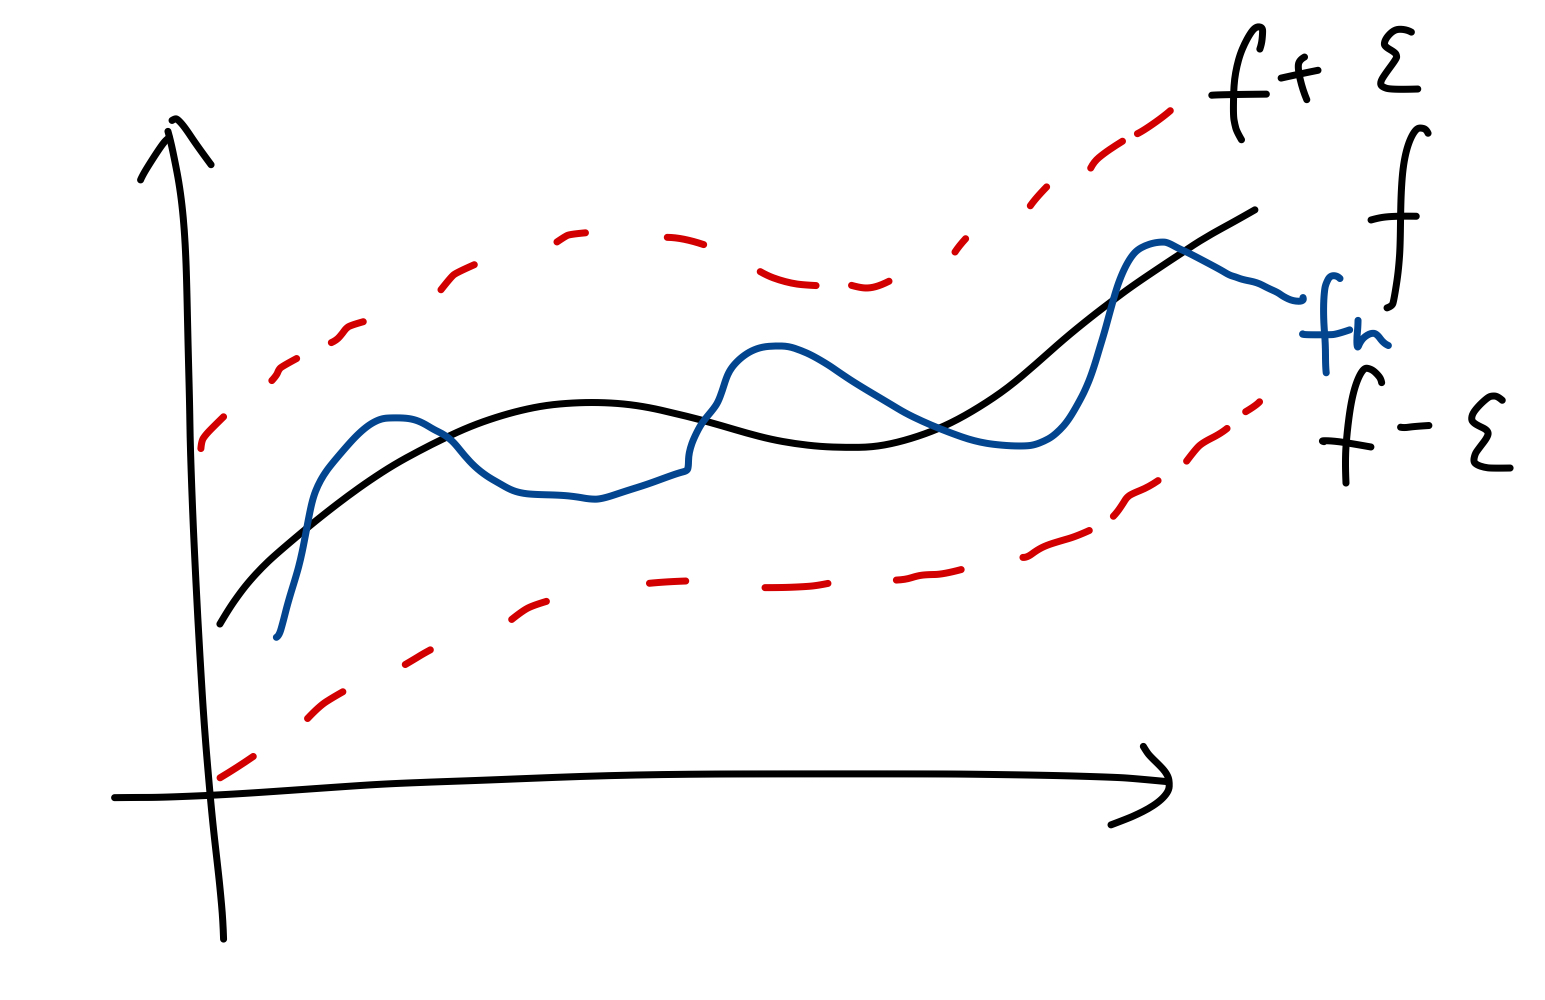
\includegraphics[scale=0.11]{at1.jpeg}
    \end{center}
\end{definition}

\begin{remark}\
    \begin{enumerate}
        \item $ N $ only depends on $\epsilon$!
        \item Uniform convergence implies pointwise convergence.
        \item Can replace $\mathbb{R}$ with $\mathbb{C}$ and can restrict to a subset of the domain.
        \item An equivalent definition of $f_{n} \rightarrow f$ uniformly on $S$ :
        \[
        \forall \varepsilon>0 \quad \exists N \in \mathbb{N} \quad \forall n \geqslant N \quad \sup _{x \in S}\left|f_{n}(x)-f(x)\right|<\varepsilon
        \]
        Even shorter: $\sup _{x \in S}\left|f_{n}(x)-f(x)\right| \rightarrow 0$ as $n \rightarrow \infty$
        \item The uniform limit $f$ if exists is unique.
    \end{enumerate}
\end{remark}

\begin{example}
\begin{enumerate}
    \item $f_{n}(x)=x^{2} \cdot e^{-n x}$ for $x \in[0, \infty)$, and $n \in \mathbb{N}$. We saw that $f_{n} \rightarrow f=0$ pointwise on $[0, \infty)$.
    \[
    0 \leqslant f_{n}(x)=\frac{x^{2}}{e^{n x}}=\frac{x^{2}}{1+n x+\frac{n^{2} x^{2}}{2}+\ldots} \leqslant \frac{2}{n^2}
    \]
    Thus,
    \[
    \sup _{x \in[0, \infty)}\left|f_{n}(x)-f(x)\right|=\sup _{x \in[0, \infty)} f_{n}(x) \leqslant \frac{2}{n^{2}} \rightarrow 0 \quad \text { as } \quad n \rightarrow \infty
    \]
    So $f_{n} \rightarrow 0$ uniformly on $[0, \infty)$.

    Could have used differentiation above to find the supremum, but the above method of finding an upper bound is better.
    \item $f_{n}(x)=x^{n}$ for $x \in[0,1], n \in \mathbb{N}$.
    We know that $f_{n} \rightarrow f$ pointwise on $[0,1]$, where
    \[
        f(x)= \begin{cases}0 & \text { if } 0 \leqslant x<1 \\ 1 & \text { if } x=1\end{cases}.
    \]
    Let $\varepsilon=1 / 2$. For any $n \in \mathbb{N}$, setting $x=\varepsilon^{1 / n}$, we have $f_{n}(x)=\varepsilon$, and so $\left|f_{n}(x)-f(x)\right| \geqslant \varepsilon$. So $f_{n} \not \rightarrow  f$ uniformly on $[0,1]$.

    Better: Since $f_{n}(1)=1$ and $f_{n}$ is continuous, there exist $\delta>0$ such that $\left|f_{n}(x)-1\right|<1 / 2$ for $x \in(1-\delta, 1+\delta)$. So for any $x \in[0,1]$ with $1-\delta<x<1$, we have $\left|f_{n}(x)-f(x)\right| \geqslant \varepsilon$.
\end{enumerate}
\end{example}
Q: Does $\left(f_{n}\right)$ converge uniformly on $S ?$
\subsection*{Strategy}
First check if $\left(f_{n}\right)$ converges pointwise on $S$.

If it doesn't, then $\left(f_{n}\right)$ does not converge uniformly on $S$.

If it does, then compute the pointwise limit $f$, and then it remains to check whether
\[
\sup _{x \in S}\left|f_{n}(x)-f(x)\right| \rightarrow 0 \quad \text { as } \quad n \rightarrow \infty
\]

If the above holds, then $f_{n} \rightarrow f$ uniformly on $S$, otherwise $\left(f_{n}\right)$ does not converge uniformly on $S$.

\begin{remark}
    What does it mean that $f_{n} \not \rightarrow f$ uniformly on $S$? We have to negate the sentence
    \[
    \forall \varepsilon>0 \quad \exists N \in \mathbb{N} \quad \forall n \geqslant N \quad \forall x \in S \quad\left|f_{n}(x)-f(x)\right|<\varepsilon
    \]
    The negation is
    \[
    \exists \varepsilon>0 \quad \forall N \in \mathbb{N} \quad \exists n \geqslant N \quad \exists x \in S \quad\left|f_{n}(x)-f(x)\right| \geqslant \varepsilon
    \]
\end{remark}

\subsection{Continuity, differentiability, and integrability}

The next theorem says that uniform limit of continuous functions is continuous.
\begin{theorem}\label{thm:1}
    Let $S$ be a subset of $\mathbb{R}$ or $\mathbb{C}$. Assume $f_{n} \rightarrow f$ uniformly on $S$. If $f_{n}$ is continuous for every $n \in \mathbb{N}$, then $f$ is continuous.
\end{theorem}
\textit{Idea}: Given $a \in S$, we want that $f(x) \approx f(a)$ provided $x \approx a$. We first choose large $n$ so that $f_{n}(x) \approx f(x)$ for every $x \in S$. Since $f_{n}$ is continuous, we have $f_{n}(x) \approx f_{n}(a)$ provided $x \approx a$. Thus, if $x \approx a$, then $f(x) \approx f_{n}(x) \approx f_{n}(a) \approx f(a)$.

\begin{proof}
    Fix $ a\in S, \epsilon>0 $. The goal is to find a $ \delta $ s.t. 
    \[
        \forall x\in S\quad |x-a|<\delta \Longrightarrow |f(x)-f(a)|<\epsilon.
    \]
    Since $ f_n\to f $ uniformly on $S$, $ \exists n\in \mathbb{N} $ such that 
    \[
        \forall x\in S\quad |f_n(x)-f(x)|<\epsilon.
    \]
    Since $f_n$ is continuous, $ \exists \delta>0 $, 
    \[
        \forall x\in S\quad |x-a|<\delta \Longrightarrow |f_n(x)-f_n(a)|<\epsilon.
    \]
    Thus for any $x\in S$, if $ |x-a|<\delta $,
    \[
        |f(x)-f(a)|\le |f(x)-f_n(x)|+|f_n(x)-f_n(a)|+|f_n(a)-f(a)|<3\epsilon.\qedhere
    \]
\end{proof}
\begin{remark}
    \begin{enumerate}
        \item It is not true for pointwise convergence. A counterexample is $x^n$.
        \item The result does not extend to differentiability.
        \item It follows that $x^{n}$ does not converge uniformly on $[0,1]$.
        \item The above proof is sometimes called a $3 \varepsilon$-proof.
        \item $\displaystyle \lim _{x \rightarrow a} \lim _{n \rightarrow \infty} f_{n}(x)=\lim _{x \rightarrow a} f(x)=f(a)=\lim _{n \rightarrow \infty} f_{n}(a)=\lim _{n \rightarrow \infty} \lim _{x \rightarrow a} f_{n}(x)$. i.e. we can \textit{swap limits} for uniformly convergent functions.
    \end{enumerate}
\end{remark}

\begin{lemma}\label{lemma 2}
    Let $S$ be any set and $f_{n}$ be a bounded function on $S$ for every $n \in \mathbb{N}$. If $f_{n} \rightarrow f$ uniformly on $S$, then $f$ is also bounded on $S$.
\end{lemma}
\begin{proof}
    Fix $n \in \mathbb{N}$ so that $\left|f_{n}(x)-f(x)\right| \leqslant 1$ for every $x \in S$. We can do this, since $f_{n} \rightarrow f$ uniformly on $S$. Since $f_{n}$ is bounded, there is an $M \in \mathbb{R}$ such that $\left|f_{n}(x)\right| \leqslant M$ for every $x \in S$. It follows that for every $x \in S$, we have
    \[
    |f(x)| \leqslant\left|f(x)-f_{n}(x)\right|+\left|f_{n}(x)\right| \leqslant 1+M
    \]
    Thus, $f$ is bounded by $M+1$.
\end{proof}

Before the next theorem, we recall some definitions and results from Analysis I. Assume $f:[a, b] \rightarrow \mathbb{R}$ is a bounded function. Given a dissection $\mathcal{D}: a=x_{0}<x_{1}<\cdots<x_{n}=b$ of $[a, b]$, the upper and lower sums of $f$ with respect to $\mathcal{D}$ are defined as
\[
U_{\mathcal{D}}(f)=\sum_{k=1}^{n}\left(x_{k}-x_{k-1}\right) \sup _{\left[x_{k-1}, x_{k}\right]} f \quad \text { and } \quad L_{\mathcal{D}}(f)=\sum_{k=1}^{n}\left(x_{k}-x_{k-1}\right) \inf _{\left[x_{k-1}, x_{k}\right]} f
\]
Riemann's criterion states that $f$ is integrable if and only if for every $\varepsilon>0$ there is a dissection $\mathcal{D}$ of $[a, b]$ such that
\[
U_{\mathcal{D}}(f)-L_{\mathcal{D}}(f)=\sum_{k=1}^{n}\left(x_{k}-x_{k-1}\right)\left(\sup _{\left[x_{k-1}, x_{k}\right]} f-\inf _{\left[x_{k-1}, x_{k}\right]} f\right)<\varepsilon
\]
An easy exercise shows that for an interval $I \subset[a, b]$ we have
\[
\sup _{I} f-\inf _{I} f=\sup _{x, y \in I}(f(x)-f(y))=\sup _{x, y \in I}|f(x)-f(y)|
\]
(This quantity is sometimes called the oscillation of $f$ on $I$.)

\begin{theorem}\label{theorem 3}
    Assume $f_{n}:[a, b] \rightarrow \mathbb{R}$ is Riemann-integrable for every $n \in \mathbb{N}$. If $f_{n} \rightarrow f$ uniformly on $[a, b]$, then $f$ is also Riemann-integrable on $[a, b]$, and moreover
    \[
    \int_{a}^{b} f_{n} \rightarrow \int_{a}^{b} f \quad \text { as } n \rightarrow \infty.
    \]
\end{theorem}

\begin{proof}
    We are going to prove that $f$ is bounded and that it satisfies Riemann's criterion. By definition of integrability, each $f_{n}$ is bounded, and hence so is $f$ by Lemma \ref{lemma 2}.
    Next, fix $\varepsilon>0$. Since $f_{n} \rightarrow f$ uniformly on $[a, b]$, we can fix $n \in \mathbb{N}$ so that $\left|f_{n}(x)-f(x)\right|<\varepsilon$ for all $x \in[a, b]$. Since $f_{n}$ is integrable, it satisfies Riemann's criterion, so there is a dissection $\mathcal{D}$ of $[a, b]$ such that $U_{\mathcal{D}}\left(f_{n}\right)-L_{\mathcal{D}}\left(f_{n}\right)<\varepsilon$. If $I$ is one of the sub-intervals of $\mathcal{D}$, then for any $x, y \in I$ we have
    \[
    \begin{aligned}
    |f(x)-f(y)| & \leqslant\left|f(x)-f_{n}(x)\right|+\left|f_{n}(x)-f_{n}(y)\right|+\left|f_{n}(y)-f(y)\right| \\
    &<\left|f_{n}(x)-f_{n}(y)\right|+2 \varepsilon
    \end{aligned}
    \]
    It follows that
    \[
    \sup _{x, y \in I}|f(x)-f(y)| \leqslant \sup _{x, y \in I}\left|f_{n}(x)-f_{n}(y)\right|+2 \varepsilon
    \]
    Multiplying both sides with the length of $I$ and summing over all sub-intervals $I$ of $\mathcal{D}$, we obtain
    \[
    U_{\mathcal{D}}(f)-L_{\mathcal{D}}(f) \leqslant U_{\mathcal{D}}\left(f_{n}\right)-L_{\mathcal{D}}\left(f_{n}\right)+2 \varepsilon(b-a)<(2(b-a)+1) \varepsilon.
    \]
    So $f$ satisfies Riemann's criterion, and thus, $f$ is integrable.
    Finally, we estimate
    \[
    \left|\int_{a}^{b} f_{n}-\int_{a}^{b} f\right| \leqslant \int_{a}^{b}\left|f_{n}-f\right| \leqslant(b-a) \sup _{[a, b]}\left|f_{n}-f\right| \rightarrow 0 \quad \text { as } n \rightarrow \infty .\qedhere
    \]
\end{proof}
\begin{remark}
    $\int_{a}^{b} \lim _{n \rightarrow \infty} f_{n}(x) \mathrm{d} x=\lim _{n \rightarrow \infty} \int_{a}^{b} f_{n}(x) \mathrm{d} x$. i.e. for uniformly convergent functions we can swap limits and integrals.
\end{remark}

\begin{corollary}\label{col:4}
    Let $f_{n}:[a, b] \rightarrow \mathbb{R}$ be an integrable function for each $n \in \mathbb{N}$. If $\sum_{n=1}^{\infty} f_{n}(x)$ converges uniformly on $[a, b]$, then $\sum_{n=1}^{\infty} f_{n}(x)$ defines an integrable function on $[a, b]$, and moreover
    \[
    \int_{a}^{b} \sum_{n=1}^{\infty} f_{n}(x) \mathrm{d} x=\sum_{n=1}^{\infty} \int_{a}^{b} f_{n}(x) \mathrm{d} x.
    \]
\end{corollary}
\begin{proof}
    Define $F_{n}(x)=\sum_{k=1}^{n} f_{k}(x)$ for $x \in[a, b]$ and $n \in \mathbb{N}$. To say that $\sum_{n=1}^{\infty} f_{n}(x)$ converges uniformly on $[a, b]$ means that $\left(F_{n}\right)$ converges uniformly on $[a, b]$. So for each $x \in[a, b]$, the series $\sum_{n=1}^{\infty} f_{n}(x)$ is convergent, and the function $x \mapsto \sum_{n=1}^{\infty} f_{n}(x)$ is the uniform limit of $\left(F_{n}\right)$ on $[a, b]$.

    We know that each $F_{n}$ is integrable and $\int_{a}^{b} F_{n}=\sum_{k=1}^{n} \int_{a}^{b} f_{k}$. So by Theorem 3 , the function $\sum_{n=1}^{\infty} f_{n}(x)$ is integrable and
    \[
    \int_{a}^{b} \sum_{n=1}^{\infty} f_{n}(x) \mathrm{d} x=\lim _{n \rightarrow \infty} \int_{a}^{b} F_{n}(x) \mathrm{d} x=\lim _{n \rightarrow \infty} \sum_{k=1}^{n} \int_{a}^{b} f_{k}(x) \mathrm{d} x=\sum_{k=1}^{\infty} \int_{a}^{b} f_{k}(x) \mathrm{d} x.\qedhere
    \]
\end{proof}

However, even uniform convergence does not guarantee differentiability. 
\begin{example}
    Let 
    \[
        f_n(x) = \begin{cases}
        |x| &\text{if }|x|\ge \frac{1}{n}\\
        \frac{n}{2}x^2+\frac{1}{2n} &\text{if }|x|<\frac{1}{n}\\
        \end{cases} \quad f(x) = |x|
    \]
    Then $ f_n\to f $ uniformly, but $f$ is not differentiable at $0$. 

    Indeed, if $ |x|\ge \frac{1}{n}, |f_n(x)-f(x)|=0 $. If $ |x|<\frac{1}{n} $, we have 
    \begin{align*}
        |f_n(x)-f(x)| &= \left| \frac{n}{2}x^2+\frac{1}{2n}-|x| \right| \\ 
        &\le \frac{n}{2}x^2+\frac{1}{2n} +|x| \\ 
        &\le \frac{n}{2}\left( \frac{1}{n} \right) +\frac{1}{2n}+\frac{1}{n}
        =\frac{2}{n}. 
    \end{align*}
    So 
    \[
        \sup_{x\in (-1,1)}|f_n(x)-f(x)| \le \frac{2}{n}\to 0, 
    \]
    and $f_n\to f$ uniformly. 
\end{example}

\begin{theorem}\label{thm:5}
    Let $\left(f_{n}\right)$ be a sequence of continuously differentiable functions on $[a, b]$. Assume further that
    \begin{enumerate}
        \item $\sum_{n=1}^{\infty} f_{n}^{\prime}(x)$ converges uniformly on $[a, b]$;
        \item there exists $c \in[a, b]$ such that $\sum_{n=1}^{\infty} f_{n}(c)$ converges.
    \end{enumerate}
    Then $\sum_{n=1}^{\infty} f_{n}(x)$ converges uniformly to a continuously differentiable function $f$ on $[a, b]$, and moreover, we have
    \[
    f^{\prime}(x)=\sum_{n=1}^{\infty} f_{n}^{\prime}(x) \quad \text { for all } x \in[a, b].
    \]
\end{theorem}
\begin{note}
    Informally, $\displaystyle \frac{\mathrm{d}}{\mathrm{d}x}\left( \sum_{n=1}^{\infty}f_n(x) \right) = \sum_{n=1}^{\infty}\frac{\mathrm{d}f_n}{\mathrm{d}x}  $. 
\end{note}
\begin{proof}
    Let $g(x)=\sum_{n=1}^{\infty} f_{n}^{\prime}(x)$ for $x \in[a, b]$. Idea: solve the equation $f^{\prime}=g$ with initial condition $f(c)=\sum_{n=1}^{\infty} f_{n}(c)$.

    Since $\sum_{n=1}^{\infty} f_{n}^{\prime}(x)$ converges uniformly to $g(x)$, and since $f_{n}^{\prime}$ is continuous for every $n \in \mathbb{N}$, by Theorem \ref{thm:1}, $ g$ is continuous, and hence integrable. Let $\lambda=\sum_{n=1}^{\infty} f_{n}(c)$ and define
    \[
    f(x)=\lambda+\int_{c}^{x} g(t)\, \mathrm{d} t \quad \text { for } x \in[a, b]
    \]
    Since $g$ is continuous, by the Fundament Theorem of Calculus (FTC) $f$ is differentiable with $f^{\prime}=g$, and moreover $f(c)=\lambda$. By the FTC we also have
    \[
    f_{k}(x)=f_{k}(c)+\int_{c}^{x} f_{k}^{\prime}(t)\, \mathrm{d} t \quad \text { for } x \in[a, b], k \in \mathbb{N}
    \]
    Given $\varepsilon>0$, by our assumptions there exists $N \in \mathbb{N}$ such that
    \[
    \begin{array}{rll}
    \displaystyle \left|\lambda-\sum_{k=1}^{n} f_{k}(c)\right| & <\varepsilon & \forall n \geqslant N \\[15pt]
    \displaystyle \left|g(t)-\sum_{k=1}^{n} f_{k}^{\prime}(t)\right| & <\varepsilon & \forall n \geqslant N \quad \forall t \in[a, b]
    \end{array}
    \]
    It follows that for all $n \geqslant N$ and for all $x \in[a, b]$ we have
    \[
    \begin{aligned}
    \left|f(x)-\sum_{k=1}^{n} f_{k}(x)\right| &=\left|\lambda+\int_{c}^{x} g(t)\, \mathrm{d} t-\sum_{k=1}^{n}\left(f_{k}(c)+\int_{c}^{x} f_{k}^{\prime}(t) \,\mathrm{d} t\right)\right| \\
    &=\left|\lambda-\sum_{k=1}^{n} f_{k}(c)+\int_{c}^{x}\left(g(t)-\sum_{k=1}^{n} f_{k}^{\prime}(t)\right) \mathrm{d} t\right| \\
    & \leqslant\left|\lambda-\sum_{k=1}^{n} f_{k}(c)\right|+\left|\int_{c}^{x}\left(g(t)-\sum_{k=1}^{n} f_{k}^{\prime}(t)\right) \mathrm{d} t\right| \\
    &<\varepsilon+(b-a) \varepsilon.
    \end{aligned}
    \]
    This shows that $\sum_{k=1}^{n} f_{k}(x) \rightarrow f(x)$ uniformly on $[a, b]$. We have already seen that $f$ is differentiable and $f^{\prime}=g$ is continuous.
\end{proof}

By considering partial sums in theorem \ref{thm:5} we get 
\begin{theorem}
    Let $(f_n)$ be a sequence of continuously differentiable functions on $[a,b]$ and assume that 
    \begin{enumerate}
        \item $f'_n$ converges uniformly to $g$ on $[a,b]$, 
        \item $f_n$ converges pointwise to $f$.
    \end{enumerate}
    Then $f$ is differentiable and $ f'=g $. 
\end{theorem}

\subsection{Uniform Cauchy}

We recall from Analysis I: a scalar sequence $\left(x_{n}\right)$ is Cauchy if
\[
\forall \varepsilon>0 \quad \exists N \in \mathbb{N} \quad \forall m, n \geqslant N \quad\left|x_{m}-x_{n}\right|<\varepsilon.
\]
The General Principle of Convergence (GPC): every Cauchy sequence is convergent.
\begin{definition}
    Let $\left(f_{n}\right)$ be a sequence of scalar functions on a set $S$. We say $\left(f_{n}\right)$ is uniformly Cauchy on $S$ if
    \[
    \forall \varepsilon>0 \quad \exists N \in \mathbb{N} \quad \forall m, n \geqslant N \quad \forall x \in S \quad\left|f_{m}(x)-f_{n}(x)\right|<\varepsilon.
    \]
\end{definition}

\begin{theorem}[General Principle of Uniform Convergence (GPUC)]\label{thm:6}
    If $\left(f_{n}\right)$ is a uniformly Cauchy sequence of scalar functions on a set $S$, then $\left(f_{n}\right)$ converges uniformly to some function $f$ on $S$.
\end{theorem}

\begin{proof}
    We first show that $\left(f_{n}\right)$ converges pointwise on $S$. Fix $x \in S$. Given $\varepsilon>0$ since $\left(f_{n}\right)$ is uniformly Cauchy, there exists $N \in \mathbb{N}$ such that
    \[
    \forall m, n \geqslant N \quad \forall t \in S \quad\left|f_{m}(t)-f_{n}(t)\right|<\varepsilon.
    \]
    In particular, for all $m, n \geqslant N$, we have $\left|f_{m}(x)-f_{n}(x)\right|<\varepsilon$. Thus, $\left(f_{n}(x)\right)_{n=1}^{\infty}$ is a Cauchy sequence, and hence convergent by the GPC. Set $f(x)=\lim _{n \rightarrow \infty} f_{n}(x)$. Doing this for every $x \in S$, we obtain a function $f$ on $S$.
    We claim that $f_{n} \rightarrow f$ uniformly on $S$. Then we will be done. 
    
    Given $\varepsilon>0$, since $\left(f_{n}\right)$ is uniformly Cauchy, there exists $N \in \mathbb{N}$ such that
    \[
    \forall m, n \geqslant N \quad \forall x \in S \quad\left|f_{m}(x)-f_{n}(x)\right|<\varepsilon.
    \]
    Fix $n \geqslant N$ and $x \in S$. Since $\left|f_{m}(x)-f_{n}(x)\right|<\varepsilon$ for every $m \geqslant N$, letting $m \rightarrow \infty$, we obtain $\left|f(x)-f_{n}(x)\right| \leqslant \varepsilon$. Since this holds for every $n \geqslant N$ and for every $x \in S$, we are done.
\end{proof}
\begin{theorem}[The Weierstrass $M$-test]\label{thm:7}
    Let $\left(f_{n}\right)$ be a sequence of scalar functions on a set $S$. Let $\sum_{n} M_{n}$ be a convergent series of non-negative real numbers. Assume that $\left|f_{n}(x)\right| \leqslant M_{n}$ for every $x \in S$ and $n \in \mathbb{N}$. Then $\sum_{n} f_{n}(x)$ converges uniformly on $S$.
\end{theorem}
\begin{proof}
    Set $F_{n}(x)=\sum_{k=1}^{n} f_{k}(x)$ for $x \in S$ and $n \in \mathbb{N}$. For $n \geqslant m$ and $x \in S$ we have
    \[
    \left|F_{m}(x)-F_{n}(x)\right| \leqslant\left|\sum_{k=m+1}^{n} f_{k}(x)\right| \leqslant \sum_{k=m+1}^{n}\left|f_{k}(x)\right| \leqslant \sum_{k=m+1}^{n} M_{k}
    \]
    Given $\varepsilon>0$, choose $N \in \mathbb{N}$ such that $\sum_{k=N}^{\infty} M_{k}<\varepsilon$. Then by the above, for every $x \in S$ and every $n \geqslant m \geqslant N$ in $\mathbb{N}$, we have
    \[
    \left|F_{m}(x)-F_{n}(x)\right| \leqslant \sum_{k=m+1}^{n} M_{k}<\varepsilon
    \]
    So $\left(F_{n}\right)$ is uniformly Cauchy, and hence uniformly convergent by Theorem \ref{thm:6}.
\end{proof}

\begin{definition}
    Let $X \subseteq \mathbb{R}$ and let $f_n:X\to \mathbb{R}$ for each $n\ge 1$. We say $(f_n)$ is \textbf{pointwise bounded} if 
    \[
        \exists M\quad \forall n\quad |f_n(x)|\le M. 
    \]
    We say $(f_n)$ is \textbf{uniformly bounded} if 
    \[
        \exists M \quad \forall x\quad \forall n \quad |f_n(x)|\le M. 
    \]
\end{definition}

\begin{note}
    Bolzano-Weierstrass theorem DOES NOT work (in uniform context). A counterexample is 
    \[
        f_n(x) = \begin{cases}
        1 &\text{if }x = n\\
        0 &\text{if }x\neq n\\
        \end{cases} 
    \]
\end{note}

\subsection{Application in power series}

Consider a power series $\sum_{n=0}^{\infty} c_{n}(z-a)^{n}$. Here $\left(c_{n}\right)_{n=0}^{\infty}$ is a complex sequence, a, $z \in \mathbb{C}$. We think of $\left(c_{n}\right)$ and $a$ as fixed, and $z$ as a variable.
Let $R$ be the radius of convergence of this power series. This means:
$|z-a|<R \quad \Longrightarrow \quad \sum_{n=0}^{\infty} c_{n}(z-a)^{n}$ converges absolutely, and hence converges, $|z-a|>R \Longrightarrow \sum_{n=0}^{\infty} c_{n}(z-a)^{n}$ diverges.

Denote $D(a, R)=\{z \in \mathbb{C}:|z-a|<R\}$, the open disk of centre $a$ and radius $R$. Consider the function
\[
f: D(a, R)  \rightarrow \mathbb{C},\quad
f(z) =\sum_{n=0}^{\infty} c_{n}(z-a)^{n}.
\]
The power series converges pointwise to $f$.

Q: Does the power series converge uniformly inside the radius of convergence?

A: In general, NO.

\begin{example}
\begin{enumerate}
    \item $\sum_{n=1}^{\infty} \frac{z^{n}}{n^{2}}$ for $|z|<1$
    Consider $f_{n}: D(0,1) \rightarrow \mathbb{C}$ define by $f_{n}(z)=z^{n} / n^{2}$. Note that $\left|f_{n}(z)\right| \leqslant 1 / n^{2}$ for all $|z|<1$. Moreover, $\sum_{n=1}^{\infty} \frac{1}{n^{2}}$ converges. Hence by the Weierstrass $M$-test, the power series converges uniformly on $D(0,1)$.
    
    \item $\sum_{n=0}^{\infty} z^{n}=\frac{1}{1-z}$ for $|z|<1$.
    $\left|\sum_{n=0}^{N} z^{n}\right| \leqslant N+1$ for $|z|<1$ and $N \in \mathbb{N} .$ So the partial sum functions are bounded on $D(0,1)$. However, $\frac{1}{1-z}$ is not bounded on $D(0,1)$. By Lemma \ref{lemma 2}, the convergence cannot be uniform on $D(0,1)$.
    Alternatively,
    \[
    \sup _{|z|<1}\left|\sum_{n=0}^{N} z^{n}-\frac{1}{1-z}\right|=\sup _{|z|<1}\left|\frac{z^{N+1}}{1-z}\right|=\infty.
    \]
\end{enumerate}
\end{example}
\begin{theorem}\label{thm:8}
    Let $\sum_{n=0}^{\infty} c_{n}(z-a)^{n}$ be a power series with radius of convergence $R$. Then for any $r$ with $0<r<R$, the power series $\sum_{n=0}^{\infty} c_{n}(z-a)^{n}$ converges uniformly on $D(a, r)=\{z \in \mathbb{C}:|z-a|<r\}$
\end{theorem}
\begin{proof}
    Fix $w \in D(a, R)$ with $r<|w-a|<R$. (E.g., $\left.w=a+\frac{r+R}{2} .\right)$ Set $\rho=\frac{r}{|w-a|}$. Since $\sum_{n=0}^{\infty} c_{n}(w-a)^{n}$ converges, we must have $c_{n}(w-a)^{n} \rightarrow 0$ as $n \rightarrow \infty$. It follows that the sequence $\left(c_{n}(w-a)^{n}\right)_{n=0}^{\infty}$ is bounded. Thus, there exists $M \geqslant 0$ such that $\left|c_{n}(w-a)^{n}\right| \leqslant M$ for all $n \geqslant 0$. Now, for any $z \in D(a, r)$ and $n \in \mathbb{N}$, we have
    \[
    \left|c_{n}(z-a)^{n}\right|=\left|c_{n}(w-a)^{n}\right| \cdot\left|\frac{(z-a)^{n}}{(w-a)^{n}}\right| \leqslant M \frac{r^{n}}{|(w-a)|^{n}}=M \rho^{n}
    \]
    Since $\sum_{n=0}^{\infty} M \rho^{n}$ converges, by Theorem \ref{thm:7}(the Weierstrass $M$-test) the power series $\sum_{n=0}^{\infty} c_{n}(z-a)^{n}$ converges uniformly on $D(a, r)=\{z \in \mathbb{C}:|z-a|<r\}$.
\end{proof}
\begin{remark}
    \begin{enumerate}
        \item The function $f: D(a, R) \rightarrow \mathbb{C}, f(z)=\sum_{n=0}^{\infty} c_{n}(z-a)^{n}$ is continuous on $D(a, r)$ for any $0<r<R$ being the uniform limit of continuous functions (polynomials). This is by Theorem \ref{thm:1}. Since $D(a, R)=\bigcup_{0<r<R} D(a, r), f$ is continuous on $D(a, R)$.
        
        \item  The power series $\sum_{n=1}^{\infty} c_{n} n(z-a)^{n-1}$ also has radius of convergence $R$ (from Analysis I). Hence it converges uniformly on $D(a, r)$ for any $0<r<R$. By an analogue of Theorem \ref{thm:5} we can deduce that $f$ is complex differentiable on $D(a, R)$ and
        \[
        f^{\prime}(z)=\frac{\mathrm{d}}{\mathrm{d} z}\left(\sum_{n=0}^{\infty} c_{n}(z-a)^{n}\right)=\sum_{n=1}^{\infty} c_{n} n(z-a)^{n-1}
        \]
        See Complex Analysis.
    
        \item Given $w \in D(a, R)$, fix $r$ with $|w-a|<r<R$ and $\delta>0$ with $|w-a|+\delta<r$. Then $D(w, \delta) \subset D(a, r) .$ Indeed, given $z \in D(w, \delta)$,
        \[
        |z-a| \leqslant|z-w|+|w-a|<\delta+|w-a|<r
        \]
        So $z \in D(a, r)$. It follows that the power series $\sum_{n=0}^{\infty} c_{n}(z-a)^{n}$ converges uniformly on $D(w, \delta)$.
    \end{enumerate}
\end{remark}
\begin{definition}
    A subset $U$ of $\mathbb{C}$ is open if for every $w \in U$ there is a $\delta>0$ such that $D(w, \delta) \subset U$
\end{definition}

\begin{definition}
    Let $U$ be an open subset of $\mathbb{C}$. A sequence $\left(f_{n}\right)$ of scalar functions on $U$ converges \textit{locally uniformly} on $U$ if for every $w \in U$ there is a $\delta>0$ such that $D(w, \delta) \subset U$ and $f_{n} \rightarrow f$ uniformly on $D(w, \delta)$
\end{definition}

\begin{remark}
    \begin{enumerate}
        \item We will return to this concept after covering compactness.
        \item Above we proved that a power series converges locally uniformly inside the radius of convergence.
    \end{enumerate}
\end{remark}

\subsection{Uniform Continuity}
We next turn to the topic of Uniform Continuity. We begin by recalling the notion of continuity from Analysis I.
Let $U$ be a subset of $\mathbb{R}$ or $\mathbb{C}$ and let $f$ be a scalar function on $U$. For $x \in U$, we say $f$ is continuous at $x$ if
\[
\forall \varepsilon>0 \quad \exists \delta>0 \quad \forall y \in U \quad|y-x|<\delta \Longrightarrow|f(y)-f(x)|<\varepsilon.
\]
We say $f$ is continuous on $U$ if $f$ is continuous at $x$ for every $x \in U$, i.e.,
\[
    \forall x \in U \quad \forall \varepsilon>0 \quad \exists \delta>0 \quad \forall y \in U \quad|y-x|<\delta \Longrightarrow|f(y)-f(x)|<\varepsilon.
\]
\begin{note}
    $\delta$ depends on $\varepsilon$ and on $x$.
\end{note}

\begin{definition}
    Let $U$ be a subset of $\mathbb{R}$ or $\mathbb{C}$ and let $f$ be a scalar function on $U$. We say $f$ is uniformly continuous on $U$ if
\[
\forall \varepsilon>0 \quad \exists \delta>0 \quad \forall x, y \in U \quad|y-x|<\delta \Longrightarrow|f(y)-f(x)|<\varepsilon
\]
\end{definition}

\begin{note}
    $\delta$ depends only on $\varepsilon$. So uniform continuity implies continuity.
\end{note}

\begin{example}
    \begin{enumerate}
        \item Consider $f: \mathbb{R} \rightarrow \mathbb{R}, f(x)=2x+17$. Given $\varepsilon>0$, set $\delta=\varepsilon / 2$. Then for every $x, y \in \mathbb{R}$, if $|x-y|<\delta$, then
        \[
        |f(x)-f(y)|=2|x-y|<2 \delta=\varepsilon
        \]
        So $f$ is uniformly continuous on $\mathbb{R}$.
        \item Consider $f: \mathbb{R} \rightarrow \mathbb{R}, f(x)=x^{2}$. Given $\varepsilon=1$, we try to find $\delta>0$ that works. Consider any $x>0$ and $y=x+\frac{\delta}{2}$. Then $|x-y|=\delta / 2<\delta$ and
        \[
        |f(x)-f(y)|=(x+\delta / 2)^{2}-x^{2}=x \delta+\delta^{2} / 4
        \]
        So for any $\delta>0$, if $x=1 / \delta$ and $y=x+\delta / 2$, then $|x-y|<\delta$ but $|f(x)-f(y)|>\varepsilon$. So $f$ is not uniformly continuous, but $f$ is continuous on $\mathbb{R}$.
    \end{enumerate}
\end{example}

\begin{note}
    A function $f$ on a subset $U$ of $\mathbb{R}$ or $\mathbb{C}$ is NOT uniformly continuous if
    \[
        \forall \varepsilon>0 \quad \exists \delta>0 \quad \forall x, y \in U \quad|x-y|<\delta \Longrightarrow|f(x)-f(y)|<\varepsilon
    \]
    is FALSE, that is
    \[
        \exists \varepsilon>0 \quad \forall \delta>0 \quad \exists x, y \in U \quad|x-y|<\delta \text{ and }|f(x)-f(y)| \geqslant \varepsilon
    \]
\end{note}
\begin{theorem}\label{thm:9}
    Let $f$ be a scalar function on a closed, bounded interval $[a, b]$. If $f$ is continuous on $[a, b]$, then $f$ is uniformly continuous on $[a, b]$. 
\end{theorem}
One idea: Let $\varepsilon>0$. For each $x \in[a, b]$ there is a $\delta_{x}>0$ such that if $|y-x|<\delta_{x}$ then $|f(y)-f(x)|<\varepsilon$. We want to take $\delta=\inf _{x} \delta_{x} .$ We might have $\delta=0$. Instead, we work indirectly: argue by contradiction.
\begin{proof}
    Assume there is an $\varepsilon>0$ such that
    \[
        \forall \delta>0 \quad \exists x, y \in[a, b] \quad|x-y|<\delta \text{ and }|f(x)-f(y)| \geqslant \varepsilon
    \]
    In particular, for every $n \in \mathbb{N}$, there exist $x_{n}, y_{n} \in[a, b]$ such that $\left|x_{n}-y_{n}\right|<1 / n$ and $\left|f\left(x_{n}\right)-f\left(y_{n}\right)\right| \geqslant \varepsilon$. By Bolzano-Weierstrass there is a subsequence $\left(x_{k_{n}}\right)_{n}$ of $\left(x_{n}\right)$ that converges to some $x \in[a, b]$. Then
    \[
    \left|y_{k_{n}}-x\right| \leqslant\left|y_{k_{n}}-x_{k_{n}}\right|+\left|x_{k_{n}}-x\right| \leqslant 1 / n+\left|x_{k_{n}}-x\right| \rightarrow 0
    \]
    Since $f$ is continuous at $x, f\left(x_{k_{n}}\right) \rightarrow f(x)$ and $f\left(y_{k_{n}}\right) \rightarrow f(x)$. Hence 
    \[
        \varepsilon \leqslant\left|f\left(x_{k_{n}}\right)-f\left(y_{k_{n}}\right)\right| \rightarrow|f(x)-f(x)|=0,
    \]
    which is a contradiction.
\end{proof}
\begin{corollary}\label{col:10}
    Let $f:[a, b] \rightarrow \mathbb{R}$ be a continuous function. Then $f$ is integrable.
\end{corollary}
\begin{proof}
    $f$ is bounded since it is continuous on the closed bounded interval $[a, b]$. It remains to verify Riemann's criterion.

    Given $\varepsilon>0$, since $f$ is uniformly continuous by Theorem \ref{thm:9}, there is a $\delta>0$ such that $|f(x)-f(y)|<\varepsilon$ whenever $|x-y|<\delta$.
    
    Next, choose a dissection $\mathcal{D}$ of $[a, b]$ such that every subinterval of $\mathcal{D}$ has length strictly less than $\delta$. (E.g. choose $n$ with $\frac{b-a}{n}<\delta$ and let $\mathcal{D}$ consist of $a+k \frac{b-a}{n}, k=0,1, \ldots, n$.) If $I$ is a subinterval of $\mathcal{D}$, then for all $x, y \in I$, we have $|x-y|<\delta$, and hence $|f(x)-f(y)|<\varepsilon$. It follows that
    \[
    \sup _{1} f-\inf _{1} f=\underset{x, y \in I}{\sup }|f(x)-f(y)| \leqslant \varepsilon
    \]
    Multiplying both sides by the length of $I$, and summing over all $I$, we obtain
    \[
    U_{\mathcal{D}}(f)-L_{\mathcal{D}}(f) \leqslant(b-a) \varepsilon.\qedhere
    \]
\end{proof}

\section{Metric Spaces}
\subsection{Definition of metric spaces}
In $\mathbb{R}$ or $\mathbb{C}$, we measure the ``closeness'' of points $x$ and $y$ by the expression $|x-y|$. A frequently used property of this ``distance'' is the triangle-inequality. We will now generalize this concept.

\begin{definition}
    Let $M$ be a set. A \textit{metric} on $M$ is a function $d: M \times M \rightarrow \mathbb{R}$ satisfying
    \begin{enumerate}[(i)]
        \item $\forall x, y \in M, d(x, y) \geqslant 0$ and $d(x, y)=0 \Longleftrightarrow x=y$\hfill (positivity)
        \item $\forall x, y \in M, d(x, y)=d(y, x)$\hfill (symmetry)
        \item $\forall x, y, z \in M, d(x, z) \leqslant d(x, y)+d(y, z)$\hfill(triangle-inequality)
    \end{enumerate}
    A \textit{metric space} is a pair $(M, d)$, where $M$ is a set and $d$ is a metric on $M$.
\end{definition}
\begin{example}
    \begin{enumerate}
        \item $M=\mathbb{R}$ or $\mathbb{C},\ d(x, y)=|x-y|$. We refer to this as the usual metric on $M$ and will always be used unless otherwise stated.
        \item $M=\mathbb{R}^{n}$ or $\mathbb{C}^{n} .$ We define the euclidean norm or euclidean length of a vector $x \in M$ by
        \[
        \|x\|=\|x\|_{2}=\left(\sum_{k=1}^{n}\left|x_{k}\right|^{2}\right)^{1 / 2}
        \]
        This satisfies the inequality $\|x+y\| \leqslant\|x\|+\|y\|$. It follows that
        \[
        d(x, y)=d_{2}(x, y)=\|x-y\|=\left(\sum_{k=1}^{n}\left|x_{k}-y_{k}\right|^{2}\right)^{1 / 2}
        \]
        defines a metric on $M$ called the euclidean metric. E.g. we check the triangle-inequality:
        \[
        d(a, c)=\|a-c\|=\|a-b+b-c\| \leqslant\|a-b\|+\|b-c\|=d(a, b)+d(b, c).
        \]
        The resulting metric space $(M, d)$ is called $n$-dimensional real or complex Euclidean space. $M$ will always be equipped with the Euclidean metric unless otherwise stated. The metric space $(M, d)$ is sometimes denoted by $\ell_{2}^{n}$ and $d_{2}$ is also called the $\ell_{2}$-metric, and $\|\cdot\|_{2}$ is also called $\ell_{2}$-norm.
        \item $M=\mathbb{R}^{n}$ or $\mathbb{C}^{n} .$ We define the $\ell_{1}$-norm of a vector $x \in M$ by
        \[
        \|x\|_{1}=\sum_{k=1}^{n}\left|x_{k}\right|
        \]
        and the corresponding metric, called the $\ell_{1}$-metric, is given by
        \[
        d_{1}(x, y)=\|x-y\|_{1}=\sum_{k=1}^{n}\left|x_{k}-y_{k}\right|
        \]
        The metric space $\left(M, d_{1}\right)$ is denoted by $\ell_{1}^{n}$. It is not hard to see how to generalize this further. For any $1 \leqslant p<\infty$ one can define the $\ell_{p}$-norm by
        \[
        \|x\|_{p}=\left(\sum_{k=1}^{n}\left|x_{k}\right|^{p}\right)^{1 / p}
        \]
        and the corresponding $\ell_{p}$-metric by $d_{p}(x, y)=\|x-y\|_{p} .$ In this course, we will only deal with $p=1,2$. (For the general case, see Part II Linear Analysis).

        Question: How about $p=\infty ?$
        \item Letting $p \rightarrow \infty$ in the previous example leads to the $\ell_{\infty}$-norm and to the $\ell_{\infty}$-metric on $M=\mathbb{R}^{n}$ or $\mathbb{C}^{n}:$
        \[
        \|x\|_{\infty}=\max _{1 \leqslant k \leqslant n}\left|x_{k}\right|\quad \text {and}\quad d_{\infty}(x, y)=\|x-y\|_{\infty}=\max _{1 \leqslant k \leqslant n}\left|x_{k}-y_{k}\right|
        \]
        The metric space $\left(M, d_{\infty}\right)$ is denoted by $\ell_{\infty}^{n}$.
        \item Let $S$ be a set. We denote by $\ell_{\infty}(S)$ the set of all bounded scalar functions on $S$. We define the $\ell_{\infty}$-norm (or uniform norm, or sup norm) of a function $f \in \ell_{\infty}(S)$ by
        \[
        \|f\|=\|f\|_{\infty}=\sup \{|f(x)|: x \in S\}
        \]
        (The sup exists since $f$ is bounded: $\exists C \geqslant 0, \forall x \in S,|f(x)| \leqslant C$.) Note that for $f, g \in \ell_{\infty}(S)$ and for any $x \in S$, we have
        \[
        |f(x)+g(x)| \leqslant|f(x)|+|g(x)| \leqslant\|f\|+\|g\|
        \]
        and hence $\|f+g\| \leqslant\|f\|+\|g\|$. It follows that $d(f, g)=\|f-g\|_{\infty}$ defines a metric, called the uniform metric (or $\ell_{\infty}$-metric) on $\ell_{\infty}(S)$.
        
        Note that $\ell_{\infty}^{n}=\ell_{\infty}(\{1,2, \ldots, n\})$. Also, $\ell_{\infty}(\mathbb{N})$ is often denoted simply $\ell_{\infty}$. This is the space of bounded scalar sequences.
        \item $C[a, b]$ denotes the space of continuous scalar functions on the closed bounded interval $[a, b]$. Let $p=1$ or 2 . We define the $L_{p}$-norm on $C[a, b]$ by
        \[
        \|f\|_{p}=\left(\int_{a}^{b}|f(t)|^{p} \mathrm{~d} t\right)^{1 / p} \quad(f \in C[a, b])
        \]
        The corresponding metric $d_{p}(f, g)=\|f-g\|_{p}$ is the $L_{p}$-metric on $C[a, b]$. E.g., for $f, g \in C[a, b]$ we have
        \[
        \|f+g\|_{1}=\int_{a}^{b}|f+g| \leqslant \int_{a}^{b}|f|+|g|=\int_{a}^{b}|f|+\int_{a}^{b}|g|=\|f\|_{1}+\|g\|_{1}
        \]
        which implies the triangle-inequality for $d_{1}$.
        \item Let $M$ be any set. For $x, y \in M$ we define
        \[
        d(x, y)= \begin{cases}0 & \text { if } x=y \\ 1 & \text { if } x \neq y\end{cases}
        \]
        This is called the discrete metric on $M$ and $(M, d)$ is a discrete metric space.
        \item Let $G$ be a group generated by $S \subset G$. Then
        \[
        d(x, y)=\min \left\{n: \exists s_{1}, \ldots, s_{n} \in S,\ y=x s_{1} s_{2} \cdots s_{n}\right\}
        \]
        is a metric called the \textit{word metric} on $G$ (Geometric Group Theory).
        \item Fix a prime $p$ in $\mathbb{Z}$. For $x, y \in \mathbb{Z}$ write $x-y=p^{n} m$ where $m, n \in \mathbb{Z}, n \geqslant 0$ and $p \nmid m$; then define
        \[
        d(x, y)= \begin{cases}0 & \text { if } x=y \\ p^{-n} & \text { if } x \neq y\end{cases}
        \]
        This is called the $p$-adic metric (Number Theory). This is in fact an ultrametric which means that for any $x, y, z$ the following holds:
        \[
        d(x, z) \leqslant \max \{d(x, y), d(y, z)\}
        \]
        which implies the triangle-inequality. A set equipped with an ultrametric is called an ultrametric space.
    \end{enumerate}
\end{example}

\subsection{Subspaces and products}
\begin{definition}[Subspaces]
    Let $(M, d)$ be a metric space and let $N \subset M$. Then $d\upharpoonright_{N \times N}$ (the restriction of $d$ to $N \times N$ ) is a metric on $N$. $N$ with this metric is called a \textit{subspace} of $(M, d)$. With a slight abuse of notation, we write $d$ both for the metric on $M$ and the metric $d \upharpoonright _{N \times N}$ on $N$.
\end{definition}
\begin{example}
    \begin{enumerate}
        \item $\mathbb{Q}$ with metric $d(x, y)=|x-y|$ is a subspace of $\mathbb{R}$.
        \item Since every continuous function on a closed bounded interval is bounded, $C[a, b]$ is a subset of $\ell_{\infty}([a, b])$. So $C[a, b]$ with the uniform metric is a subspace of $\ell_{\infty}([a, b])$.
    \end{enumerate}
\end{example}

\begin{definition}[Products]
    Let $(M, d)$ and $\left(M^{\prime}, d^{\prime}\right)$ be a metric spaces. Then any of the following define a metric on $M \times M^{\prime}:$
    \[
    \begin{aligned}
    d_{1}\left(\left(x, x^{\prime}\right),\left(y, y^{\prime}\right)\right) &=d(x, y)+d^{\prime}\left(x^{\prime}, y^{\prime}\right) \\
    d_{2}\left(\left(x, x^{\prime}\right),\left(y, y^{\prime}\right)\right) &=\left(d(x, y)^{2}+d^{\prime}\left(x^{\prime}, y^{\prime}\right)^{2}\right)^{1 / 2} \\
    d_{\infty}\left(\left(x, x^{\prime}\right),\left(y, y^{\prime}\right)\right) &=\max \left\{d(x, y), d^{\prime}\left(x^{\prime}, y^{\prime}\right)\right\}
    \end{aligned}
    \]
    The metric space $\left(M \times M^{\prime}, d_{p}\right)$ is denoted $M \oplus_{p} M^{\prime}(p=1,2, \infty)$. This can be generalized to the product of any finite number of metric spaces
    \[
        \left( \bigoplus_{k=1}^{n}M_k \right)_p = M_1 \oplus_{p}M_2\oplus_{p}\cdots\oplus_{p}M_n
    \]
    with metric
    \[
        d_p((x_1,\dots,x_n),(y_1,\dots,y_n)) = \left( \sum_{k=1}^n d_k(x_k,y_k)^p \right)^{1/p}.
    \]
\end{definition}
\begin{note}
    $d_{\infty} \leqslant d_{2} \leqslant d_{1} \leqslant 2 d_{\infty}$.
\end{note}
\begin{example}
    \[
\mathbb{R} \oplus_{1} \mathbb{R}=\ell_{1}^{2} \quad \mathbb{R} \oplus_{2} \mathbb{R} \oplus_{2} \mathbb{R}=\ell_{2}^{3} \quad \underbrace{\mathbb{R} \oplus_\infty \cdots \oplus_{\infty} \mathbb{R}}_{n \text { times }}=\ell_{\infty}^{n}
\]
However, $\mathbb{R} \oplus_{1} \mathbb{R} \oplus_{2} \mathbb{R}$ makes no sense as $\left(\mathbb{R} \oplus_{1} \mathbb{R}\right) \oplus_{2} \mathbb{R}$ and $\mathbb{R} \oplus_{1}\left(\mathbb{R} \oplus_{2} \mathbb{R}\right)$ are different.
\end{example}
\subsection{Convergence}
Convergence has the exact same meaning. 
\begin{definition}[Convergence]
    Let $M$ be a metric space and let $\left(x_{n}\right)$ be a sequence in $M$. Given $x \in M$, we say $\left(x_{n}\right)$ converges to $x$ and write $x_{n} \rightarrow x$ as $n \rightarrow \infty$ if
    \[
    \forall \varepsilon>0 \quad \exists N \in \mathbb{N} \quad \forall n \geqslant N \quad d\left(x_{n}, x\right)<\varepsilon
    \]
    We say $\left(x_{n}\right)$ is convergent in $M$ if there is an $x \in M$ such that $\left(x_{n}\right)$ converges to $x$. We say $\left(x_{n}\right)$ is divergent if it is not convergent.
\end{definition}

\begin{note}
    $x_{n} \rightarrow x \Longleftrightarrow d\left(x_{n}, x\right) \rightarrow 0$.
\end{note}
\begin{lemma}[Uniqueness of limit]\label{lma:1}
    Assume that $x_{n} \rightarrow x$ and $x_{n} \rightarrow y$ in a metric space $M$. Then $x=y$.
\end{lemma}

\begin{proof}
    Suppose not. Set $\varepsilon=d(x, y) / 3 .$ Then $\varepsilon>0$, and so we can choose $N_{1}$ and $N_{2}$ in $\mathbb{N}$ such that
    \[
    \forall n \geqslant N_{1} \quad d\left(x_{n}, x\right)<\varepsilon \quad \text { and } \quad \forall n \geqslant N_{2} \quad d\left(x_{n}, y\right)<\varepsilon
    \]
    Fix any $n \geqslant \max \left\{N_{1}, N_{2}\right\} .$ Then we have
    \[
    d(x, y) \leqslant d\left(x, x_{n}\right)+d\left(x_{n}, y\right)<2 \varepsilon<d(x, y)
    \]
    which is a contradiction.
\end{proof}

\begin{definition}
    Given a convergent sequence $\left(x_{n}\right)$ in a metric space $M$, the limit of $\left(x_{n}\right)$ (denoted by $\lim _{n \rightarrow \infty} x_{n}$ ) is the unique $x \in M$ such that $x_{n} \rightarrow x$ as $n \rightarrow \infty$.
\end{definition}

\begin{example}
    \begin{enumerate}
        \item In $\mathbb{R}$ and $\mathbb{C}$ convergence has the usual meaning.
        \item Constant sequences converge. More generally, assume $\left(x_{n}\right)$ is an eventually constant sequence in a metric space $M$ : there is an $N \in \mathbb{N}$ and $x \in M$ such that $x_{n}=x$ for $n \geqslant N$. Then $x_{n} \rightarrow x$ as $n \rightarrow \infty$.
        The converse is false: e.g., $\frac{1}{n} \rightarrow 0$ in $\mathbb{R}$.

        However, assume $x_{n} \rightarrow x$ in a discrete metric space. Then there is an $N \in \mathbb{N}$ such that $d\left(x_{n}, x\right)<1$ for $n \geqslant N$, and hence $x_{n}=x$ for $n \geqslant N$.
        \item In the 3-adic metric on $\mathbb{Z}, 3^{n} \rightarrow 0$ as $n \rightarrow \infty$ since $d\left(3^{n}, 0\right)=3^{-n} \rightarrow 0$ as $n \rightarrow \infty$
        \item Let $S$ be a set. In $\ell_{\infty}(S),\ f_{n} \rightarrow f$ in the uniform metric if and only if $d\left(f_{n}, f\right)=\left\|f_{n}-f\right\|_{\infty}=\sup _{s}\left|f_{n}-f\right| \rightarrow 0$ as $n \rightarrow \infty$. This is equivalent to saying that $f_{n} \rightarrow f$ uniformly on $S$.
        
        Note that if $f_{n}(x)=x+\frac{1}{n}$ and $f(x)=x$ for $x \in \mathbb{R}$ and $n \in \mathbb{N}$, then $f_{n} \rightarrow f$ uniformly on $\mathbb{R}$, but $f_{n}, f \notin \ell_{\infty}(\mathbb{R})$.
        \item Consider Euclidean $ \bbR^n $ or $ \bbC^n $ with $ \ell_2 $-metric. Note that for $ \bfx^{(k)}=(x_1^{(k)},\dots,x_n^{(k)}) $ and $ \bfx=(x_1,\dots,x_n) $, we have 
        \[
            | x_i^{(k)}-x_i | \le \| \bfx^{(k)}-\bfx \| \le \sum_{i=1}^{n}| x_i^{(k)}-x_i |.
        \]
        So $ \bfx^{(k)}\to \bfx \Longleftrightarrow $ for every $i$, $ x_i^{(k)}\to x_i $. This is called \textit{coordinate-wise convergence}.
        \item Consider $\mathbb{R}^{\mathbb{N}}$, the set of all real sequences. Check that for sequences $x=\left(x_{k}\right)$ and $y=\left(y_{k}\right)$
        \[
        d(x, y)=\sum_{k=1}^{\infty} 2^{-k} \min \left\{1,\left|x_{k}-y_{k}\right|\right\}
        \]
        defines a metric on $\mathbb{R}^{\mathbb{N}}$. Then a sequence $\left(x^{(n)}\right)$ in $\mathbb{R}^{\mathbb{N}}$ converges to $x \in \mathbb{R}^{\mathbb{N}}$ if and only if $x_{k}^{(n)} \rightarrow x_{k}$ as $n \rightarrow \infty$ for each $k \in \mathbb{N} .\left(x^{(n)}=\left(x_{k}^{(n)}\right)_{k=1}^{\infty}\right)$ 
        
        Q: Given any set $S$, is there a metric on $\mathbb{R}^{S}$ such that convergence in the metric is equivalent to pointwise convergence on $S ?$
        \item Consider $f_{n}(x)=x^{n}$ for $x \in[0,1]$ and $n \in \mathbb{N}$. Then $\left(f_{n}\right)$ is a sequence in $C[0,1]$. Recall that $\left(f_{n}\right)$ converges pointwise but not uniformly on $[0,1]$. Thus, $\left(f_{n}\right)$ does not converge in the uniform metric. However,
        \[
        d_{1}\left(f_{n}, 0\right)=\left\|f_{n}\right\|_{1}=\int_{0}^{1}\left|f_{n}\right|=\frac{1}{n+1} \rightarrow 0
        \]
        and so $f_{n} \rightarrow 0$ in $C[0,1]$ in the $L_{1}$-metric.
        \item Let $M$ be a metric space, $N$ a subspace of $M$ and $\left(x_{n}\right)$ a sequence in $N$. If $\left(x_{n}\right)$ is convergent in $N$, then $\left(x_{n}\right)$ is convergent in $M$. The converse is false. E.g., $\frac{1}{n} \rightarrow 0$ in $\mathbb{R}$, but $\left(\frac{1}{n}\right)$ does not converge in $(0, \infty)$.
        \item Let $M$ and $M^{\prime}$ be metric spaces and consider $N=M \oplus_{p} M^{\prime}$ where $p=1,2$ or $\infty$. Let $\left(a_{n}\right)$ be a sequence in $N$ and write $a_{n}=\left(x_{n}, x_{n}^{\prime}\right)$ where $x_{n} \in M$ and $x_{n}^{\prime} \in M^{\prime} .$ Let $a=\left(x, x^{\prime}\right) \in N$. Then
        \[
        a_{n} \rightarrow a \text { in } N \Longleftrightarrow x_{n} \rightarrow x \text { in } M \text { and } x_{n}^{\prime} \rightarrow x^{\prime} \text { in } M^{\prime}
        \]
        This follows easily from the following:
        \[
        \begin{aligned}
        \max \left\{d\left(x_{n}, x\right), d^{\prime}\left(x_{n}^{\prime}, x^{\prime}\right)\right\}&=d_{\infty}\left(a_{n}, a\right) \\
        &\le d_{p}\left(a_{n}, a\right) \\
        & \leqslant d_{1}\left(a_{n}, a\right)=d\left(x_{n}, x\right)+d^{\prime}\left(x_{n}^{\prime}, x^{\prime}\right).
        \end{aligned}
        \]
        E.g., In $\mathbb{R}^{n}$, we have $v_{i}=\left(x_{i, 1}, \ldots, x_{i, n}\right) \rightarrow v=\left(x_{1}, \ldots, x_{n}\right)$ iff $x_{i, k} \rightarrow x_{k}$ as $i \rightarrow \infty$ for each $k=1, \ldots, n$.
    \end{enumerate}
\end{example}

\subsection{Continuity}\ \vspace{-1.5em}
\begin{definition}
    Consider a function $f: M \rightarrow M^{\prime}$ between metric spaces $M$ and $M^{\prime}$. For $a \in M$ we say $f$ is continuous at $a$ if
    \[
    \forall \varepsilon>0 \quad \exists \delta>0 \quad \forall x \in M \quad d(x, a)<\delta \Longrightarrow d^{\prime}(f(x), f(a))<\varepsilon
    \]
    We say $f$ is continuous if $f$ is continuous at $a$ for every $a \in M$, i.e.,
    \[
    \forall a \in M \quad \forall \varepsilon>0 \quad \exists \delta>0 \quad \forall x \in M \quad d(x, a)<\delta \Longrightarrow d^{\prime}(f(x), f(a))<\varepsilon
    \]
\end{definition}
\begin{note}
    $\delta$ depends on $\varepsilon$ and on $a$.
\end{note}
More generally, for a subset $N \subset M$ we say $f$ is continuous on $N$ if $f$ is continuous at every $a \in N$.
\begin{note}
    $f$ being continuous on $N$ is related to but is different from $f\restriction_N: N \rightarrow M^{\prime}$ being continuous. The former implies the latter, but the converse fails.
$f$ continuous on $N$ means:
    \[
        \forall a \in N \quad \forall \varepsilon>0 \quad \exists \delta>0 \quad \forall x \in M \quad d(x, a)<\delta \Longrightarrow d^{\prime}(f(x), f(a))<\varepsilon
    \]
    $f\restriction_N: N \rightarrow M^{\prime}$ continuous means:
    \[
        \forall a \in N \quad \forall \varepsilon>0 \quad \exists \delta>0 \quad \forall x \in N \quad d(x, a)<\delta \Longrightarrow d^{\prime}(f(x), f(a))<\varepsilon
    \]
\end{note}

\begin{example}
$M=\mathbb{R}$ and $f: \mathbb{R} \rightarrow \mathbb{R}, x \mapsto \begin{cases}0 & \text { if } x<0 \\ 1 & \text { if } x \geqslant 0\end{cases}$

$N=[0, \infty)$ and then $f\restriction_N:[0, \infty) \rightarrow \mathbb{R}, x \mapsto 1$, is a constant function, so clearly continuous. However, $f$ is not continuous on $N$, e.g., $f$ is not continuous at 0.
\end{example}

\begin{proposition}
	Let \( f \colon M \to M' \) be as above.
	Let \( a \in M \).
	Then the following are equivalent:
	\begin{enumerate}[(i)]
		\item \( f \) is continuous at \( a \);
		\item \( x_n \to a \) in \( M \) implies \( f(x_n) \to f(a) \) in \( M \)
	\end{enumerate}
    So if $f$ is continuous, then for every convergent sequence $\left(x_n\right)$ in $M,\left(f\left(x_n\right)\right)$ is convergent in $M^{\prime}$, and moreover $\lim _{n \rightarrow \infty} f\left(x_n\right)=f\left(\lim _{n \rightarrow \infty} x_n\right)$.
\end{proposition}
\begin{proof}
	First we show (i) implies (ii).
	Suppose \( x_n \to a \) in \( M \).
	Then fix \( \varepsilon > 0 \), and seek \( N \in \mathbb N \) such that \( \forall n \geq N, d'(f(x_n), f(a)) < \varepsilon \).
	By continuity, there exists \( \delta > 0 \) such that \( \forall x \in M, d(x,a) < \delta \implies d'(f(x_n), f(a)) < \varepsilon \) as required.
	So we want \( N \) such that \( \forall n \geq N, d(x,a) < \delta \), which must exist since \( x_n \to a \).

	Now, we show (ii) implies (i).
	Suppose that \( f \) is not continuous at \( a \).
	Then,
	\[
		\exists \varepsilon > 0, \forall \delta > 0, \exists x \in M, d(x,a) < \delta, d'(f(x), f(a)) \geq \varepsilon
	\]
	So fix such an \( \varepsilon \) for which no suitable \( \delta \) exists.
	Choose the sequence \( \delta_n = \frac{1}{n} \), so
	\[
		d(x_n,a) < \frac{1}{n};\quad d'(f(x_n), f(a)) \geq \varepsilon
	\]
	Then \( x_n \to a \) in \( M \) but \( f(x_n) \not\to f(a) \) in \( M \), which is a contradiction.
\end{proof}

\begin{proposition}
	Let \( f,g \) be scalar functions on a metric space \( M \).
	Let \( a \in M \).
	Then if \( f,g \) are continuous at \( a \), so are \( f+g \) and \( f \cdot g \).
	Moreover, letting \( N = \qty{x \in M \colon g(x) \neq 0} \) and assuming \( a \in N \), \( \frac{f}{g} \) is continuous at \( a \).
	Hence if \( f,g \) are continuous, then so are \( f+g, f \cdot g, \frac{f}{g} \) where they are defined.
\end{proposition}
\begin{proof}
	Suppose \( x_n \to a \).
	Then by the above proposition, \( (f\cdot g)(x_n) = f(x_n) \cdot g(x_n) \to f(a) \cdot g(a) = (f \cdot g)(a) \), and similar results hold for the other operators.
\end{proof}
\begin{remark}
	If \( f \colon M \to M' \) is continuous everywhere,
	\[
		\lim_{n \to \infty} f(x_n) = f\qty(\lim_{n \to \infty} x_n)
	\]
	by the second proposition.
\end{remark}
\begin{proposition}
	Let \( f \colon M \to M', g \colon M' \to M'' \) be functions between metric spaces.
	If \( f \) is continuous at \( a \) and \( g \) is continuous at \( f(a) \), then \( g \circ f \) is continuous at \( a \).
	If \( f,g \) are continuous, \( g \circ f \) is continuous.
\end{proposition}
\begin{proof}
	Let \( \varepsilon > 0 \).
	We want to find \( \delta > 0 \) such that \( \forall x \in M \), \( d(x,a) < \delta \) implies \( d''(g(f(x)), g(f(a))) < \varepsilon \).
	Since \( g \) is continuous at \( f(a) \), there exists \( \eta > 0 \) such that \( \forall y \in M' \), \( d'(y,f(a)) < \eta \implies d''(g(y), g(f(a))) < \varepsilon \).
	Now, since \( f \) is continuous at \( a \), for this \( \eta \) there exists \( \delta \) such that for all \( x \in M \), \( d(x,a) < \delta \implies d'(f(x) - f(a)) < \eta \).
	Then \( d(x,a) < \delta \implies d''(g(f(x)), g(f(a))) < \varepsilon \) as required.
\end{proof}

\begin{definition}
	Let \( f \colon M \to M' \) be a function between metric spaces.
	Then, \( f \) is
	\begin{enumerate}
		\item \textbf{isometric}, if \( \forall x,y \in M, d'(f(x),f(y)) = d(x,y) \)
		\item \textbf{Lipschitz}, or \( c \)-Lipschitz, if \( \exists c \in \mathbb R^+, \forall x,y \in M, d'(f(x),f(y)) \leq c\cdot d(x,y) \)
		\item \textbf{uniformly continuous}, if \( \forall \varepsilon > 0, \exists \delta > 0, \forall x,y \in M, d(x,y) < \delta \implies d'(f(x), f(y)) < \varepsilon \)
	\end{enumerate}
\end{definition}

\begin{note}
    \begin{enumerate}
        \item isometric $\Longrightarrow$ Lipschitz $\Longrightarrow$ uniformly continuous $\Longrightarrow$ continuous.
        \item An isometric map is injective but not necessarily surjective. An isometric map that is also surjective is called an \textbf{isometry}. The inverse of an isometry is also an isometry. If there is an isometry $M \rightarrow M^{\prime}$, we say that $M$ and $M^{\prime}$ are \textbf{isometric metric spaces} or that $M^{\prime}$ is an \textbf{isometric copy} of $M$.
    \end{enumerate}
\end{note}

\begin{example}
	\begin{enumerate}
        \item Constant functions are continuous.
        For instance, let \( b \in M \) and let \( f(x) = b \).
        Then this is continuous since \( d'(f(x) - f(a)) = d'(b,b) = 0 \) so any \( \delta > 0 \) will satisfy the condition.
    
        \item The identity function \( f \colon M \to M \) defined by \( x \mapsto x \) is continuous.
        Consider \( d(f(x) - f(a)) = d(x-a) \).
        So \( \delta = \varepsilon \) will suffice.
    
        \item All real and complex polynomials and rational functions are continuous wherever they are defined by the propositions and examples above.
        In fact, using uniform convergence, the uniform limits of such functions are also continuous.
        For example, exponential and trigonometric functions are continuous.
    
        \item Let \( (M, d) \) be a metric space.
        Then \( d \colon M \oplus_p M \to \mathbb R \), which can be viewed as a function between metric spaces \( M \oplus_p M \) and \( \mathbb R \).
        Then, given \( v = (x,x'), w = (y,y') \in M \oplus_p M \),
        \begin{align*}
            \abs{d(v) - d(w)} &= \abs{d(x,x') - d(y,y')} \\ 
            &\leq d(x,y) + d(x',y') \\ 
            &= d_1(v,w) \leq 2 d_p(v,w)
        \end{align*}
        Hence \( \delta = \frac{\varepsilon}{2} \) will suffice.

        \item Let $M, M^{\prime}$ be metric spaces.
        Fix $y \in M^{\prime}$ and consider the function $f: M \rightarrow M \oplus_p M^{\prime}, f(x)=(x, y)$. 
        
        For $x, z \in M$, we have $d_p(f(x), f(z))=d_p((x, y),(z, y))=d(x, z)$, and thus $f$ is isometric, and $M \times\{y\}$ is an isometric copy of $M$.
        This generalizes to any finite number of metric spaces. For example, given $a \in \mathbb{R}^n$, the map $x \mapsto\left(a_1, \ldots, a_{k-1}, x, a_{k+1}, \ldots, a_n\right): \mathbb{R} \rightarrow \mathbb{R}^n$ is isometric.

        \begin{center}
            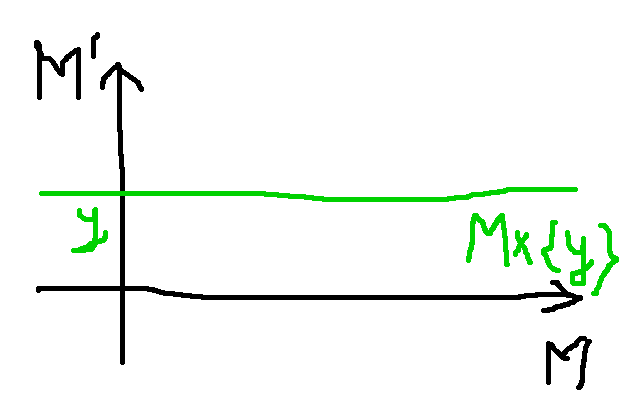
\includegraphics[scale=0.2]{at2.png}
        \end{center}
        
        \item Let $M, M^{\prime}$ be metric spaces. Consider the projection functions
        \[
            \pi: M \oplus_p M^{\prime} \rightarrow M,\left(x, x^{\prime}\right) \mapsto x \quad \text{and}\quad \pi^{\prime}: M \oplus_p M^{\prime} \rightarrow M^{\prime},\left(x, x^{\prime}\right) \mapsto x^{\prime}
        \]
        For $\mathbf{x}=\left(x, x^{\prime}\right)$ and $\mathbf{y}=\left(y, y^{\prime}\right)$ in $M \oplus_p M^{\prime}$, we have
        \[
        d(\pi(\mathbf{x}), \pi(\mathbf{y}))=d(x, y) \leqslant \max \left\{d(x, y), d^{\prime}\left(x^{\prime}, y^{\prime}\right)\right\}=d_{\infty}(\mathbf{x}, \mathbf{y}) \leqslant d_p(\mathbf{x}, \mathbf{y})
        \]
        and so $\pi$ is 1-Lipschitz. The same holds for $\pi^{\prime}$.

        E.g., $\mathbb{C}^n \rightarrow \mathbb{C},\left(z_1, \ldots, z_n\right) \mapsto z_k$ is continuous. We deduce that polynomials in any number of variables are also continuous.
    \end{enumerate}
\end{example}

\subsection{Generalised triangle inequality}
Suppose \( u,x,y,z \in M \).
Then, \( \abs{d(u,x) - d(y,z)} \leq d(u,y) + d(x,z) \).
First,
\[
	d(u,x) \leq d(u,y) + d(y,x) \leq d(u,y) + d(y,z) + d(z,x)
\]
Rearranging,
\[
	d(u,x)-d(y,z) \leq d(u,y) + d(x,z)
\]
To achieve the negative, satisfying both conditions in the absolute value term,
\[
	d(y,z) \leq d(y,u) + d(u,x) + d(x,z)
\]
which gives
\[
	d(y,z) - d(u,x) \leq d(u,y) + d(x,z)
\]
as required.

\section{Topology of metric spaces}
\subsection{Open balls}
In a metric space, continuity at a point $x$ or convergence of a sequence to a point $x$ depends on the set of points close to $x$. This motivates the following.
\begin{definition}
	Let $(M, d)$ be a metric space and $x \in M$. We define the \textbf{open ball} in $M$ with centre $x$ and radius $r$ (or the open $r$-ball around $x$ ) as the set
    \[
    D_r(x)=\{y \in M: d(y, x)<r\}
    \]
    We sometimes write $D_r^M(x)$ to indicate the underlying metric space $M$.
\end{definition}
The open ball notation is a convenient syntax for denoting closeness in some metric space.
Note that
\[
    \begin{aligned}
        &x_n \rightarrow x \text { in } M \Longleftrightarrow \forall \varepsilon>0\quad \exists N \in \mathbb{N}\quad \forall n \geqslant N \quad x_n \in D_{\varepsilon}(x) \\
        &f: M \rightarrow M^{\prime} \text { is continuous at } x \Longleftrightarrow \forall \varepsilon>0\quad \exists \delta>0\quad f\left(D_\delta(x)\right) \subset D_{\varepsilon}(f(x))
    \end{aligned}
\]
\begin{definition}
	The closed ball of centre \( x \) and radius \( r \geq 0 \) is the set
	\[
		B_r(x) = \qty{y \in M \colon d(y,x) \leq r}
	\]
\end{definition}
\begin{example} 
	\begin{enumerate}
        \item \( \mathbb R \), \( D_r(x) = (x-r,x+r) \),
        \( B_r(x) = [x-r,x+r] \).
        \item \( (\mathbb R^2, d_p) \), $\displaystyle B_1(0) = \left\{ x \in \mathbb R^2 \colon \norm{x}_p \leq 1  \right\}$. 
        \item In $\mathbb{C}, D_r(x)$ and $B_r(x)$ are the open and closed discs with centre $x$ and radius $r$.
        \item Let \( M \) be a discrete metric space.
        Then for \( x \in M \),
        \[
            D_1(x) = \qty{x};\quad B_1(x) = M
        \]
    \end{enumerate}
\end{example}
\begin{note}
	\begin{enumerate}
        \item $D_r(x) \subset B_r(x) \subset D_s(x)$ whenever $r<s$.
        \item $d(x, y)=\min \left\{r \geqslant 0: y \in B_r(x)\right\}=\inf \left\{r>0: y \in D_r(x)\right\}$
    \end{enumerate}
\end{note}

\subsection{Neighbourhoods and openness}\ \vspace{-1.5em}
\begin{definition}
	Let \( M \) be a metric space, and \( U \subset M \).
	Then for \( x \in M \), we say that \( U \) is a \textbf{neighbourhood} of \( x \) (in \( M \)) if
	\[
		\exists r > 0\quad D_r(x) \subset U \iff \exists r > 0\quad B_r(x) \subset U
	\]
\end{definition}
\begin{definition}
	We say \( U \subset M \) is \textbf{open} in \( M \), or that \( U \) is an \textbf{open subset} of \( M \), if
	\[
		\forall x \in U\quad \exists r > 0\quad D_r(x) \subset U
	\]
	So \( U \) is a neighbourhood of all points in \( U \).
\end{definition}
\begin{example}
	\( D_r(x), B_r(x) \) are neighbourhoods of \( x \).
\end{example}
\begin{example}
	Let \( H = \qty{ z \in \mathbb C \colon \Im z \geq 0 } \).
	Let \( w \in H \) and \( \delta = \Im w \).
	If \( \delta > 0 \), then \( D_\delta(w) \subset H \).
	If \( \delta = 0 \), then for any \( r \), \( D_\delta(w) \not\subset H \).
	So \( H \) is not open.
\end{example}
\begin{lemma}
	Open balls are open.
\end{lemma}
\begin{proof}
	Let \( D_r(x) \) be an open ball in a metric space \( M \).
	We need to show that
	\[
		\forall y \in D_r(x)\quad \exists \delta > 0\quad D_\delta(y) \subset D_r(x)
	\]
	So let \( y \in D_r(x) \) and set \( \delta = r - d(x,y) \).
	Note that \( d(x,y) > 0 \), and by the triangle inequality,
	\[
		d(z,x) \leq d(z,y) + d(y,x) < \delta + (r-\delta) = r
	\]
	as required.
\end{proof}
\begin{corollary}\label{col:2.6}
	Let \( M \) be a metric space, \( U \subset M \), \( x \in M \).
	Then \( U \) is a neighbourhood of \( x \) if and only if there exists an open subset \( V \) of \( M \) such that \( x \in V \subset U \).
\end{corollary}
\begin{proof}
	In the forward direction, there exists \( r > 0 \) such that \( D_r(x) \subset U \), so let \( V = D_r(x) \).
	Conversely, if \( V \) is open we can construct \( r > 0 \) such that \( D_r(x) \subset V \subset U \).
	So \( U \) is a neighbourhood of \( x \).
\end{proof}

\subsection{Continuity and convergence using topology}\ \vspace{-1.5em}
\begin{proposition}\label{prop:2.7}
	In a metric space \( M \), the following are equivalent.
	\begin{enumerate}[(i)]
		\item \( x_n \to x \);
		\item for all neighbourhoods \( U \) of \( x \) in \( M \), \( \exists N \in \mathbb N, \forall n \geq N, x_n \in U \);
		\item for all open neighbourhoods \( U \) of \( x \) in \( M \), \( \exists N \in \mathbb N, \forall n \geq N, x_n \in U \).
	\end{enumerate}
\end{proposition}
\begin{proof}
	((i) $ \Rightarrow$ (ii))
	Let \( U \) be a neighbourhood of \( x \).
	Then by definition \( \exists \varepsilon > 0, D_\varepsilon(x) \subset U \).
	Since \( x_n \to x \),
	\[
		\exists N \in \mathbb N, \forall n \geq N, x_n \in D_\varepsilon(x)
	\]
	hence \( \forall n \geq N, x_n \in U \).

	((ii) $ \Rightarrow$ (iii))
	This is clear since any open set \( U \) with \( x \in U \) is a neighbourhood of \( x \).

	((iii) $ \Rightarrow$ (i))
	Fix \( \varepsilon > 0 \).
	By the above lemma, \( U = D_\varepsilon(x) \) is open, and \( x \in U \).
	Then by (iii),
	\[
		\exists N \in \mathbb N, \forall n \geq n, x_n \in U
	\]
	hence \( d(x_n, x) < \varepsilon \).
\end{proof}
\begin{proposition}\label{prop:2.8}
	Let \( f \colon M \to M' \) be a function between metric spaces.
	\begin{enumerate}[(a)]
		\item The following are equivalent for all \( x \in M \).
		      \begin{enumerate}[(i)]
			      \item \( f \) is continuous at \( x \);
			      \item for all neighbourhoods \( V \) of \( f(x) \) in \( M' \), there exists a neighbourhood \( U \) of \( x \) in \( M \) such that \( f(U) \subset V \);
			      \item for all neighbourhoods \( V \) of \( f(x) \) in \( M' \), \( f^{-1}(V) \) is a neighbourhood of \( x \) in \( M \).
		      \end{enumerate}
		\item The following are equivalent.
		      \begin{enumerate}[(i)]
			      \item \( f \) is continuous;
			      \item \( f^{-1}(V) \) is open in \( M \) for all open subsets \( V \) of \( M' \). (The inverse image of open set is open.)
		      \end{enumerate}
	\end{enumerate}
\end{proposition}
\begin{proof}
    We begin with part (a). 
    
    We first recall that (i) is the following statement.
    \[
        \forall \varepsilon>0 \quad \exists \delta>0 \quad f\left(D_\delta(x)\right) \subset D_{\varepsilon}(f(x))
    \]

    ((i) $\Rightarrow$ (ii)) Given a neighbourhood $V$ of $f(x)$ in $M^{\prime}$, there is an $\varepsilon>0$ such that $D_{\varepsilon}(f(x)) \subset V$. Since $f$ is continuous at $x$, there is a $\delta>0$ such that $f\left(D_\delta(x)\right) \subset D_{\varepsilon}(f(x))$. Set $U=D_\delta(x)$. Then $U$ is a neighbourhood of $x$ in $M$ and $f(U) \subset D_{\varepsilon}(f(x)) \subset V$.

    ((ii) $\Rightarrow$ (iii)) Given a neighbourhood $V$ of $f(x)$ in $M^{\prime}$, by assumption (ii) there is a neighbourhood $U$ of $x$ in $M$ such that $f(U) \subset V$. By definition of neighbourhood, there is a $r>0$ such that $D_r(x) \subset U$. It follows that $D_r(x) \subset U \subset f^{-1}(V)$, and hence $f^{-1}(V)$ is a neighbourhood of $x$ in $M$.

    ((iii) $\Rightarrow$ (i)) Given $\varepsilon>0$, the set $V=D_{\varepsilon}(f(x))$ is a neighbourhood of $f(x)$ in $M^{\prime}$, and hence $f^{-1}(V)$ is a neighbourhood of $x$ in $M$ by assumption. By definition, there is a $\delta>0$ such that $D_\delta(x) \subset f^{-1}(V)$. It follows that $f\left(D_\delta(x)\right) \subset V=D_{\varepsilon}(f(x))$. 

    We now deduce part (b).

    ((i) $\Rightarrow$ (ii)) Let $V$ be an open set in $M^{\prime}$. Fix $x \in f^{-1}(V)$. Then $f(x) \in V$, and so $V$ is a neighbourhood of $f(x)$ in $M^{\prime}$. Since $f$ is continuous at $x$, it follows from (a) that $f^{-1}(V)$ is a neighbourhood of $x$ in $M$. This holds for any $x \in f^{-1}(V)$, and thus $f^{-1}(V)$ is open in $M$.

    ((ii) $\Rightarrow$ (i)) Let $x \in M$ and let $\varepsilon>0$. Since $V=D_{\varepsilon}(f(x))$ is open in $M^{\prime}$, it follows that $f^{-1}(V)$ is open in $M$ by assumption. Since $f(x) \in V$, we have $x \in f^{-1}(V)$. Thus, there is a $\delta>0$ such that $D_\delta(x) \subset f^{-1}(V)$. It follows that $f\left(D_\delta(x)\right) \subset V=D_{\varepsilon}(f(x))$. This shows that $f$ is continuous at every $x \in M$, and thus $f$ is continuous.
\end{proof}

\begin{definition}
	The \textbf{topology} of a metric space \( M \) is the family of all open subsets of \( M \).
\end{definition}
\begin{proposition}\label{prop:2.9}
	The topology of a metric space satisfies
	\begin{enumerate}[(i)]
		\item \( \varnothing \) and \( M \) are open;
		\item if \( U_i \) are open in \( M \) for \( i \in I \) (\( I \) may be countable or uncountable), then \( \bigcup_{i \in I} U_i \) is open in \( M \);
		\item if \( U, V \) are open then \( U \cap V \) is open.
	\end{enumerate}
\end{proposition}
\begin{proof}
	(ii): Let \( x \in \bigcup_{i \in I} U_i \), then \( \exists i_a \in I, x \in U_{i_a} \).
	Then since \( U_{i_a} \) is open, \( \exists \delta > 0, D_r(x) \subset U_{i_a} \subset \bigcup_{i \in I} U_i \)

	(iii) Given \( x \in U \cap V \), since \( U \) is open then \( \exists r > 0 \), \( D_r(x) \subset U \) and \( \exists s > 0 \), \( D_s(x) \subset V \).
	Then let \( t = \min(r,s) \), and \( D_t(x) = D_r(x) \cap D_s(x) \subset U \cap V \).
\end{proof}

\subsection{Properties of topology of metric space}\ \vspace{-1.5em}
\begin{definition}
	Let $M$ be a metric space and $A \subset M$. We say $A$ is closed in $M$ (or that $A$ is a closed subset of $M)$ if for every sequence $\left(x_n\right)$ in $A$ that converges in $M$, we have $\lim _{n \rightarrow \infty} x_n$ is in $A$.
\end{definition}
\begin{lemma}
	Closed balls are closed.
\end{lemma}
\begin{proof}
	Consider \( B_r(x) \) in \( M \).
	Consider further \( (x_n) \in B_r(x) \) such that \( x_n \to z \) in \( M \).
	\[
		d(z,x) \leq d(z,x_n) + d(x_n,x) \leq d(z,x_n) + r \to r
	\]
	Hence \( d(z,x) \leq r \), so \( z \in B_r(x) \).
\end{proof}
\begin{example}
	\begin{enumerate}
        \item \( [0,1] = B_{1/2}(1/2) \) is closed in \( \mathbb R \).
        This is not open, for instance consider \( D_r(0) \not\subset [0,1] \).
    
        \item \( (0,1) = D_{1/2}(1/2) \) is open in \( \mathbb R \).
        This is not closed, for instance the sequence \( \frac{1}{n+1} \to 0\) in \( \mathbb R \).
    
        \item \( \mathbb R \) and \( \varnothing \) are open and closed in \( \mathbb R \).
    
        \item \( (0,1] \) in \( \mathbb R \) is neither open nor closed.
        \( D_r(1) \not\subset (0,1] \) and \( \frac{1}{n} \to 0 \not\in (0,1] \).
    \end{enumerate}
\end{example}
\begin{lemma}\label{lma:2.11}
	Let \( A \subset M \).
	Then \( A \) is closed in \( M \) if and only if \( M \setminus A \) is open in \( M \).
\end{lemma}
\begin{proof}
	Let \( A \) be closed.
	Suppose \( M \setminus A \) is not open.
	Then \( \exists x \in M \setminus A, \forall r > 0, D_r(x) \not\subset M \setminus A \), so \( D_r(x) \cap A \neq \varnothing \).
	In particular, for every \( n \) we can choose a point in \( D_{1/n}(x) \cap A \).
	Then, \( d(x_n,x) < \frac{1}{n} \to 0 \) and \( x_n \in A \) which contradicts the fact that \( A \) is closed.

	Conversely, assume \( M \setminus A \) is open, but suppose \( A \) is not closed.
	Then there exists a sequence \( (x_n) \in A \) such that \( x_n \to x \) in \( M \) but \( x \not\in A \).
	Since \( x \in M \setminus A \) and \( M \setminus A \) is open, there exists \( \varepsilon > 0, D_\varepsilon(x) \subset M \setminus A \).
	Since \( x_n \to x \), we must have \( \exists N \in \mathbb N, \forall n \geq N, x_n \in D_\varepsilon(x) \) and hence \( x_n \in M \setminus A \), contradiction.
\end{proof}
\begin{example}
	Let \( M \) be a discrete metric space.
	Let \( A \subset M \).
	Then for all \( x \in A \), \( D_1(x) = \qty{x} \subset A \).
	Hence \( A \) is open.
	So in a discrete metric space, all subsets are open.
	Hence every subset is closed.
\end{example}

\subsection{Homeomorphisms}
Recall that a map $f: M \rightarrow M^{\prime}$ between metric spaces is an isometry if it is bijective and isometric $\left(d^{\prime}(f(x), f(y))=d(x, y)\right.$ for all $\left.x, y \in M\right)$. This is the correct notion of structure-preserving map for metric spaces provided we are interested in metric properties, i.e., properties that depend on the metric itself. What if we are only interested in the topology that comes from the metric?

\begin{definition}
	A map \( f \colon M \to M' \) between metric spaces is called a \textbf{homeomorphism} if \( f \) is a bijection and \( f, f^{-1} \) are continuous.

	Equivalently, \( f \) is a bijection, and for all open sets \( V \) in \( M' \), \( f^{-1}(V) \) is open in \( M \), and for all open sets \( U \) in \( M \), \( f(U) \) is open in \( M' \).

	If there exists a homeomorphism between \( M, M' \), we say that \( M, M' \) are \textbf{homeomorphic}.
\end{definition}
\begin{example}
	Consider \( (0,\infty) \) and \( (0,1) \).
	Consider the map \( x \mapsto \frac{1}{x+1} \) with inverse \( x \mapsto \frac{1}{x} - 1 \).
	These are continuous, so the metric spaces are homeomorphic.
\end{example}
\begin{remark}
\begin{enumerate}
    \item Every isometry is a homeomorphism. Converse is false.
    \item Isometric metric spaces are homeomorphic. Converse is false.
    \item The identity map on a metric space is a homeomorphism, the inverse of a homeomorphism is a homeomorphism and the composite of homeomorphisms is a homeomorphism. It follows that being homeomorphic is an equivalence relation.
    \item Let $f: M \rightarrow M^{\prime}$ be a homeomorphism. If $U$ is an open subset of $M$, then $f(U)=\left(f^{-1}\right)^{-1}(U)$ is open in $M^{\prime}$, and conversely, if $V$ is an open subset of $M^{\prime}$, then $f^{-1}(V)$ is open in $M$. So we have a bijection between the topologies of $M$ and $M^{\prime}$.
    \item Let $f: M \rightarrow M^{\prime}$ be a homeomorphism. Then $\left(x_n\right)$ is convergent in $M$ if and only if $\left(f\left(x_n\right)\right)$ is convergent in $M^{\prime}$. Also, $g: N \rightarrow M$ is continuous if and only if $f \circ g$ is continuous, and $h: N \rightarrow M^{\prime}$ is continuous if and only if $f^{-1} \circ h$ is continuous. Similar comment applies to functions from $M$ and $M^{\prime}$.
    \item A continuous bijection need not be a homeomorphism. E.g.,
    Id: $(\mathbb{R}$, discrete$) \rightarrow(\mathbb{R}$, euclidean$)$
\end{enumerate}
\end{remark}

\subsection{Equivalence of metrics}\ \vspace{-1.5em}
\begin{definition}
	Let \( d, d' \) be metrics on a set \( M \).
	We say that \( d, d' \) are \textbf{equivalent}, written \( d \sim d' \), if they define the same topology.
\end{definition}

\begin{remark}
	Remark Each of the following statements are equivalent to $d \sim d^{\prime}$.
\begin{enumerate}
    \item The identity map Id: $(M, d) \rightarrow\left(M, d^{\prime}\right)$ is a homeomorphism. Note that this is stronger than saying that $(M, d)$ and $\left(M, d^{\prime}\right)$ are homeomorphic.
    \item $(M, d)$ and $\left(M, d^{\prime}\right)$ have the same convergent sequences.
    \item For every metric space $N$ and every $f: N \rightarrow M, f$ is continuous with respect to $d$ if and only if it is continuous with respect to $d^{\prime}$.
    \item For every metric space $N$ and every $f: M \rightarrow N, f$ is continuous with respect to $d$ if and only it is continuous with respect to $d^{\prime}$.
\end{enumerate}
\end{remark}

\begin{definition}
	Let \( d, d' \) be metrics on \( M \).
	Then we say \( d, d' \) are \textbf{uniformly equivalent}, written \( d \sim_u d' \) if
	\[
		\mathrm{id} \colon (M, d) \to (M, d');\quad \mathrm{id} \colon (M, d') \to (M, d)
	\]
	are uniformly continuous.
	We say \( d, d' \) are \textbf{Lipschitz equivalent}, written \( d \sim_\mathrm{Lip} d' \), if the identity maps above are Lipschitz.
\end{definition}
Equivalently, \( d \sim_\mathrm{Lip} d' \) if \( \exists a > 0, b > 0, ad(x,y) \leq d'(x,y) \leq bd(x,y) \).
	Note, \( d \sim_\mathrm{Lip} d' \implies d \sim_u d' \implies d \sim d' \).
\begin{example}
	\begin{enumerate}
        \item Given \( (M,d) \), define \( d'(x,y) = \min(1,d(x,y)) \).
        This defines a metric on \( M \), and \( d' \sim_u d \).
    
        \item On \( M \times M' \), \( d_1, d_2, d_\infty \) are pairwise Lipschitz equivalent.
    
        \item Consider \( C[0,1] \).
        The \( L_1 \) metric and the uniform metric are not equivalent.
        Consider \( f_n(x) = x^n \).
        This is convergent to zero in the \( L_1 \) metric but is not convergent in the uniform metric.
    
        \item The discrete metric and Euclidean metric on \( \mathbb R \) are not equivalent.
        This is becaue in the discrete metric all sets are open, but in the Euclidean metric there are some non-open sets.
    \end{enumerate}
\end{example}

\section{Completeness}
\subsection{Cauchy sequences}
In \( \mathbb R, \mathbb C \), every Cauchy sequence is convergent.
We wish to generalise this notion to an arbitrary metric space.
Recall that a sequence \( (x_n) \) in \( \mathbb R \) or \( \mathbb C \) is bounded if there exists \( c \in \mathbb R^+ \) such that \( \forall n \in \mathbb N, \abs{x_n} \leq c \).
\begin{definition}
	A sequence \( (x_n) \) in a metric space \( M \) is said to be \textbf{Cauchy} if
	\[
		\forall \varepsilon > 0\quad \exists N \in \mathbb N\quad \forall m,n \geq N\quad d(x_m,x_n) < \varepsilon
	\]
	The sequence is bounded if
	\[
		\exists z \in M\quad \exists r > 0\quad \forall n \in \mathbb N\quad x_n \in B_r(z)
	\]
	This is equivalent to
	\[
		\forall z \in M\quad \exists r > 0\quad \forall n \in \mathbb N\quad x_n \in B_r(z)
	\]
	by considering the triangle inequality around the given \( z \) point.
	In particular, if the metric arises from a norm, \( (x_n) \) is bounded if and only if \( \norm{x_n} \) is bounded.
\end{definition}
\begin{lemma}
	$ \text { convergent } \Longrightarrow \text { Cauchy } \Longrightarrow \text { bounded } $
\end{lemma}

\begin{proof}
    Let $\left(x_n\right)$ be a sequence in a metric space $M$.

    For the first implication, assume that $\left(x_n\right)$ is convergent $M$ and let $x$ denote its limit. Given $\varepsilon>0$, there exists $N \in \mathbb{N}$ such that $d\left(x_n, x\right)<\varepsilon / 2$ for all $n \geqslant N$. Then for $m, n \geqslant N$ we have
    \[
    d\left(x_m, x_n\right) \leqslant d\left(x_m, x\right)+d\left(x, x_n\right)<\varepsilon
    \]
    Thus, $\left(x_n\right)$ is Cauchy.

    For the second implication, assume that $\left(x_n\right)$ is Cauchy. Then there exists $N \in \mathbb{N}$ such that $d\left(x_m, x_n\right) \leqslant 1$ for all $m, n \geqslant N$. It follows that $x_n \in B_1\left(x_N\right)$ for all $n \geqslant N$. Now let
    \[
    r=\max \left\{d\left(x_1, x_N\right), d\left(x_2, x_N\right), \ldots, d\left(x_{N-1}, x_N\right), 1\right\}
    \]
    Then $x_n \in B_r\left(x_N\right)$ for all $n \in \mathbb{N}$.
\end{proof}

\begin{remark}
\begin{enumerate}
    \item Bounded $\centernot\implies$ Cauchy E.g., $0,1,0,1,0,1 \ldots$ in $\mathbb{R}$
    \item Cauchy $\centernot\implies$ convergent E.g., $(1 / n)$ in $(0, \infty)$.
\end{enumerate}
\end{remark}

\subsection{Completeness}\ \vspace{-1.5em}
\begin{definition}
	A metric space \( M \) is called \textbf{complete} if every Cauchy sequence in \( M \) converges in \( M \).
\end{definition}
\begin{example}
	\( \mathbb R, \mathbb C \) are complete.
\end{example}
\begin{proposition}
    If $M$ and $M^{\prime}$ are complete metric spaces, then $M \oplus_p M^{\prime}$ is also complete for $p=1,2$ and $\infty$.
\end{proposition}
\begin{proof}
    Let $\left(a_n\right)$ be a Cauchy sequence in $M \oplus_p M^{\prime}$ where $a_n=\left(x_n, x_n^{\prime}\right)$ for $n \in \mathbb{N}$. Given $\varepsilon>0$, there exists $N \in \mathbb{N}$ such that $d_p\left(a_m, a_n\right)<\varepsilon$ for all $m, n \geqslant N$. It follows that
    \[
    d\left(x_m, x_n\right) \leqslant d_p\left(a_m, a_n\right)<\varepsilon \quad \forall m, n \geqslant N
    \]
    and hence $\left(x_n\right)$, and by a similar argument $\left(x_n^{\prime}\right)$, is Cauchy. Since $M$ and $M^{\prime}$ are complete, $x_n \rightarrow x$ and $x_n^{\prime} \rightarrow x^{\prime}$ for some $x \in M$ and $x^{\prime} \in M^{\prime}$. Finally, let $a=\left(x, x^{\prime}\right)$. Then
    \[
    d_p\left(a_n, a\right) \leqslant d\left(x_n, x\right)+d^{\prime}\left(x_n^{\prime}, x^{\prime}\right) \rightarrow 0 \quad \text { as } n \rightarrow \infty
    \]
    Thus, $\left(a_n\right)$ in convergent in $M \oplus_p M^{\prime}$.
\end{proof}
\begin{note}
    $\left(a_n\right)$ is Cauchy if and only if $\left(x_n\right)$ and $\left(x_n^{\prime}\right)$ are Cauchy.
\end{note}

\begin{corollary}
$\mathbb{R}^n$ and $\mathbb{C}^n$ are complete in the $\ell_p$-metric for $p=1,2$ and $\infty$. In particular, $n$-dimensional real or complex euclidean space is complete.
\end{corollary}

\subsection{Completeness of subspaces}\ \vspace{-1.5em}

\begin{theorem}
    Let $S$ be an arbitrary set. Then the space $\ell_{\infty}(S)$ is complete in the uniform metric $D$.
\end{theorem}
\begin{proof}
    Let $\left(f_n\right)$ be a Cauchy sequence in $\ell_{\infty}(S)$. Then given $\varepsilon>0$, there exists $N \in \mathbb{N}$ such that for all $m, n \geqslant N$, we have
    \[
        D\left(f_m, f_n\right)=\sup _{x \in S}\left|f_m(x)-f_n(x)\right|<\varepsilon \implies \forall x \in S \quad\left|f_m(x)-f_n(x)\right|<\varepsilon.
    \]
    Thus, $\left(f_n\right)$ is uniformly Cauchy, and hence converges uniformly to a scalar function $f$ on $S$. It follows that $f$ is bounded, i.e., $f \in \ell_{\infty}(S)$. Finally, since $f_n \rightarrow f$ uniformly on $S$, given $\varepsilon>0$, there exists $N \in \mathbb{N}$ such that for all $n \geqslant N$ we have
    \[
        \forall x \in S \quad\left|f_n(x)-f(x)\right|<\varepsilon \implies D\left(f_n, f\right)=\sup _{x \in S}\left|f_n(x)-f(x)\right| \leqslant \varepsilon.
    \]
    This shows that $f_n \rightarrow f$ in the uniform metric.
\end{proof}

\begin{proposition}
    Let $N$ be a subspace of a metric space $M$.
    \begin{enumerate}[(i)]
        \item If $N$ is complete, then $N$ is closed in $M$.
        \item If $M$ is complete and $N$ is closed in $M$, then $N$ is complete.
    \end{enumerate}In particular, in a complete metric space, a subspace is closed if and only if it is complete.
\end{proposition}
\begin{proof}
    (i) Given $\left(x_n\right)$ in $N$, assume $x_n \rightarrow x$ in $M$. Then $\left(x_n\right)$ is Cauchy in $M$ by Lemma 12 , and hence Cauchy in $N$. Since $N$ is complete, $x_n \rightarrow y$ for some $y$ in $N$, and hence $x_n \rightarrow y$ in $M$. By uniqueness of limit, $x=y$, and thus $x \in N$, as required.

    (ii) Let $\left(x_n\right)$ be a Cauchy sequence in $N$. Then $\left(x_n\right)$ is Cauchy in $M$, and hence $x_n \rightarrow x$ for some $x$ in $M$. Since $N$ is closed, $x$ belongs to $N$. It follows that $x_n \rightarrow x$ in $N$.
\end{proof}

\begin{definition}
    Definition Let $(M, d)$ be a metric space. We define
    \[
    C_b(M)=\left\{f \in \ell_{\infty}(M): f \text { is continuous}\right\}.
    \]
    So in the real case, we have
    \[
    C_b(M)=\{f: M \rightarrow \mathbb{R}: f \text { is bounded and continuous}\}.
    \]
\end{definition}

\begin{note}
    $C_b(M)$ is a subspace of $\ell_{\infty}(M)$ in the uniform metric $D$.
\end{note}

\begin{theorem}
    $C_b(M)$ is complete in the uniform metric for any metric space $M$.
\end{theorem}

\begin{proof}
    It is enough to show that $C_b(M)$ is closed in $\ell_{\infty}(M)$. Let $\left(f_n\right)$ be a sequence in $C_b(M)$, let $f \in \ell_{\infty}(M)$, and assume that $f_n \rightarrow f$. We need to show that $f \in C_b(M)$, i.e., that $f$ is continuous. 
    
    Fix $a \in M$ and $\varepsilon>0$. Since $f_n \rightarrow f$, we can choose a large $n \in \mathbb{N}$ such that
    \[
    D\left(f_n, f\right)=\sup _{x \in M}\left|f_n(x)-f(x)\right|<\varepsilon.
    \]
    Since $f_n$ is continuous at $a$, there exists $\delta>0$ such that
    \[
    \forall x \in M \quad d(x, a)<\delta \Longrightarrow\left|f_n(x)-f_n(a)\right|<\varepsilon.
    \]
    It follows that for any $x \in M$, if $d(x, a)<\delta$, then
    \[
    \begin{aligned}
    |f(x)-f(a)| & \leqslant\left|f(x)-f_n(x)\right|+\left|f_n(x)-f_n(a)\right|+\left|f_n(a)-f(a)\right| \\
    & \leqslant \varepsilon+\varepsilon+\varepsilon=3 \varepsilon.
    \end{aligned}
    \]
    This shows that $f$ is continuous at $a$, and hence continuous.
\end{proof}

\begin{corollary}
    For any closed, bounded interval $[a, b]$ in $\mathbb{R}$, the space $C[a, b]$ of continuous scalar functions on $[a, b]$ is complete in the uniform metric.
\end{corollary}

\begin{definition}
    Let $S$ be a set and $(N, e)$ be a metric space. Define
    \[
    \ell_{\infty}(S, N)=\{f: S \rightarrow N: f \text { is bounded}\}
    \]
    We say $f$ is bounded if: $\exists y \in N \quad \exists r>0 \quad \forall x \in S \quad f(x) \in B_r(y)$

    Now assume that $g: S \rightarrow N$ is another bounded function: there exist $z \in N$ and $s>0$ such that $g(x) \in B_s(z)$ for all $x \in S$. Then
    \[
    \forall x \in S \quad e(f(x), g(x)) \leqslant e(f(x), y)+e(y, z)+e(z, g(x)) \leqslant r+e(y, z)+s
    \]
    It follows that $\sup _{x \in S} e(f(x), g(x))$ exists and will be denoted by $D(f, g)$. It is routine to verify that $D$ is a metric on $\ell_{\infty}(S, N)$ called the \textbf{uniform metric}.

    Now assume further that $(M, d)$ is a metric space. Define
    \[
    C_b(M, N)=\{f: M \rightarrow N: f \text { is bounded and continuous}\}
    \]
    which is a subspace of $\ell_{\infty}(M, N)$.
\end{definition}

\begin{theorem}\label{thm:19}
    Let $S$ be a set, $(M, d)$ and $(N, e)$ be metric spaces, and assume $N$ is complete. Then
\begin{enumerate}[(i)]
    \item $\ell_{\infty}(S, N)$ is complete in the uniform metric.
    \item $C_b(M, N)$ is complete in the uniform metric.
\end{enumerate}
\end{theorem}

\begin{proof}
    (i) Let $\left(f_k\right)$ be a Cauchy sequence in $\ell_{\infty}(S, N)$. We first show that $\left(f_k\right)$ is pointwise convergent. 
    
    Fix $x \in S$ and $\varepsilon>0$, since $\left(f_k\right)$ is Cauchy, there exists $K \in \mathbb{N}$ such that $D\left(f_i, f_j\right)<\varepsilon$ for all $i, j \geqslant K$. It follows that
    \[
    e\left(f_i(x), f_j(x)\right) \leqslant D\left(f_i, f_j\right)<\varepsilon \quad \text { for all } i, j \geqslant K
    \]
    Hence $\left(f_k(x)\right)$ is Cauchy in $N$, and thus convergent in $N$, since $N$ is complete. We can now define $ f: S \rightarrow N \text { by } f(x)=\lim _{k \rightarrow \infty} f_k(x) $.

    We next show that $f$ is bounded. 
    
    Since $ (f_k)$ is Cauchy, $\left(f_k\right)$ is bounded in the metric space $\ell_{\infty}(S, N)$. So there exists $g \in \ell_{\infty}(S, N)$ and $r>0$ such that $f_k \in B_r(g)$ for all $k \in \mathbb{N}$. Since $g$ is bounded, there exists $y \in N$ and $s>0$ such that $g(x) \in B_s(y)$ for all $x \in S$. It follows that for any $x \in S$ and $k \in \mathbb{N}$, we have
    \[
    e\left(f_k(x), y\right) \leqslant e\left(f_k(x), g(x)\right)+e(g(x), y) \leqslant D\left(f_k, g\right)+s \leqslant r+s
    \]
    and thus $f_k(x) \in B_{r+s}(y)$. By Lemma 2.10, the set $B_{r+s}(y)$ is closed in $N$. It follows that $f(x)=\lim _{k \rightarrow \infty} f_k(x) \in B_{r+s}(y)$ for all $x \in S$, and so $f$ is bounded, i.e., $f \in \ell_{\infty}(S, N)$.

    It remains to show that $f_k \rightarrow f$ in the uniform metric in $\ell_{\infty}(S, N)$. 
    
    Let $\varepsilon>0$. Since $\left(f_k\right)$ is Cauchy, there exists $K \in \mathbb{N}$ such that $D\left(f_i, f_j\right)<\varepsilon$ for all $i, j \geqslant K$. Fix $x \in S$ and $i \geqslant K$. Then
    \[
    e\left(f_i(x), f_j(x)\right) \leqslant D\left(f_i, f_j\right)<\varepsilon \quad \text { for all } j \geqslant K
    \]
    Since $f_j(x) \rightarrow f(x)$, and since the metric $e$ is continuous, it follows that $e\left(f_i(x), f(x)\right) \leqslant \varepsilon$. Since this holds for any $x \in S$, we have $D\left(f_i, f\right) \leqslant \varepsilon$, and this is true for any $i \geqslant K$. This proves that $f_i \rightarrow f$ in the uniform metric $D$.
    
    (ii) Since $\ell_{\infty}(M, N)$ is complete, it suffices to prove that $C_b(M, N)$ is closed in $\ell_{\infty}(M, N)$. Let $\left(f_k\right)$ be a sequence in $C_b(M, N)$, let $f \in \ell_{\infty}(M, N)$, and assume that $f_k \rightarrow f$ in the uniform metric. We need to show that $f \in C_b(M, N)$, i.e., that $f$ is continuous.

    Fix $a \in M$ and $\varepsilon>0$. Since $f_k \rightarrow f$, we can choose a large $k \in \mathbb{N}$ such that
    \[
    D\left(f_k, f\right)=\sup _{x \in M} e\left(f_k(x), f(x)\right)<\varepsilon
    \]
    Since $f_k$ is continuous at $a$, there exists $\delta>0$ such that
    \[
    \forall x \in M \quad d(x, a)<\delta \Longrightarrow e\left(f_k(x), f_k(a)\right)<\varepsilon
    \]
    It follows that for any $x \in M$, if $d(x, a)<\delta$, then
    \[
    \begin{aligned}
    e(f(x), f(a)) & \leqslant e\left(f(x), f_k(x)\right)+e\left(f_k(x), f_k(a)\right)+e\left(f_k(a), f(a)\right) \\
    & \leqslant \varepsilon+\varepsilon+\varepsilon=3 \varepsilon
    \end{aligned}
    \]
    This shows that $f$ is continuous at $a$, and hence continuous.
\end{proof}

\section{Contraction mappings}
\subsection{Contraction mapping theorem}\ \vspace{-1.5em}
\begin{definition}
    A map $f: M \rightarrow M^{\prime}$ between metric spaces is called a contraction mapping if
\[
\exists \lambda<1 \quad \forall x, y \in M \quad d^{\prime}(f(x), f(y)) \leqslant \lambda d(x, y)
\]
\end{definition}
\begin{note}
    Equivalently, $f$ is $\lambda$-Lipschitz with $\lambda<1$. Thus, a contraction mapping is continuous.
\end{note}

\begin{theorem}[Contraction Mapping Theorem]
    Let $M$ be a non-empty, complete metric space and let $f: M \rightarrow M$ be a contraction mapping. Then $f$ has a unique fixed point, i.e. there is a unique $z \in M$ such that $f(z)=z$. 
\end{theorem}
\begin{proof}
    Fix $\lambda<1$ such that $d(f(x), f(y)) \leqslant \lambda d(x, y)$ for all $x, y \in M$.

    Uniqueness: Assume $f(z)=z$ and $f(w)=w$. Then
    \[
    d(z, w)=d(f(z), f(w)) \leqslant \lambda d(z, w)
    \]
    Since $\lambda<1$, it follows that $z=w$. 

    Existence: Fix an arbitrary $x_0 \in M$ and define $\left(x_n\right)_{n=1}^{\infty}$ recursively by $x_n=f\left(x_{n-1}\right)$. Thus, $x_n=f^n(x)$, $f$ applies $n$ times.

    Idea: if $z= f^{\infty}(x_0)$, then $f(z)=z$.

    For any $n \in \mathbb{N}$, we have
    \[
    d\left(x_n, x_{n+1}\right)=d\left(f\left(x_{n-1}\right), f\left(x_n\right)\right) \leqslant \lambda d\left(x_{n-1}, x_n\right) \leqslant \ldots \leqslant \lambda^n d\left(x_0, x_1\right).
    \]
    It follows that for any $m, n \in \mathbb{N}$ with $n \geqslant m$, we have
    \begin{align*}
        d\left(x_m, x_n\right) &\leqslant \sum_{k=m}^{n-1} d\left(x_k, x_{k+1}\right) \leqslant \sum_{k=m}^{n-1} \lambda^k d\left(x_0, x_1\right)\\ 
        &=\frac{\lambda^m-\lambda^n}{1-\lambda} d\left(x_0, x_1\right) \leqslant \frac{\lambda^m}{1-\lambda} d\left(x_0, x_1\right).
    \end{align*}
    Since $\frac{\lambda^m}{1-\lambda} \rightarrow 0$ as $m \rightarrow \infty$, given $\varepsilon>0$, there exists $N \in \mathbb{N}$ such that $\frac{\lambda^m}{1-\lambda} d\left(x_0, x_1\right)<\varepsilon$ for all $m \geqslant N$, and then by above $d\left(x_m, x_n\right)<\varepsilon$ whenever $n \geqslant m \geqslant N$. This show that $\left(x_n\right)$ is Cauchy. Since $M$ is complete, $x_n \rightarrow z$ for some $z \in M$.
    Since $f$ is continuous, $f\left(x_n\right) \rightarrow f(z)$ as $n \rightarrow \infty$. On the other hand, $f\left(x_n\right)=x_{n+1} \rightarrow z$, so $f(z)=z$.
\end{proof}

\begin{remark}
\begin{enumerate}
    \item The proof not only shows the existence of a fixed point, but also a way of approximating it. Letting $n \rightarrow \infty$ in the inequality for $d\left(x_m, x_n\right)$, we obtain
    \[
    d\left(x_m, z\right) \leqslant \frac{\lambda^m}{1-\lambda} d\left(x_0, x_1\right) \quad \text { for all } m \in \mathbb{N}.
    \]
    Thus, the convergence is exponentially fast.
    \item $f: \mathbb{R} \setminus\{0\} \rightarrow \mathbb{R} \setminus\{0\}, x \mapsto x / 2$ is a contraction $\left(\lambda=\frac{1}{2}\right)$ but has no fixed point.
    \item $f: \mathbb{R} \rightarrow \mathbb{R}, x \mapsto x+1$ is isometric $(\lambda=1)$ but has no fixed point.
    \item $f:[1, \infty) \rightarrow[1, \infty), x \mapsto x+\frac{1}{x}$ satisfies $|f(x)-f(y)|<|x-y|$ for all $x, y \in[1, \infty)$ but has no fixed point.
\end{enumerate}
\end{remark}

\subsection{An application: initial value problem}
Given $y_0 \in \mathbb{R}$, consider the initial value problem (IVP)
\[
f^{\prime}(t)=f\left(t^2\right), \quad f(0)=y_0.
\]
Using contraction mapping theorem, we can show that it has a unique solution given an interval. 
\begin{proposition}
    The IVP above has a unique solution on $\left[0, \frac{1}{2}\right]$. In other words, there is a unique differentiable function $f:\left[0, \frac{1}{2}\right] \rightarrow \mathbb{R}$ satisfying $f(0)=y_0$ and $f^{\prime}(t)=f\left(t^2\right)$ for all $t \in\left[0, \frac{1}{2}\right]$.
\end{proposition}
\begin{proof}
    We show this in four steps. 

    \textit{Step 1: construct $f$.} $ f$ is a solution of the IVP if and only if
        \[
        f \in C\left[0, \frac{1}{2}\right] \quad \text { and } \quad f(t)=y_0+\int_0^t f\left(s^2\right) \mathrm{d} s \quad \text {for all } t \in\left[0, \frac{1}{2}\right].
        \]

    \textit{Step 2: introduce a contraction mapping.} $ M=C\left[0, \frac{1}{2}\right]$ is a non-empty, complete metric space in the uniform metric $D$. Define $T: M \rightarrow M$ by
    \[
    T(g)(t)=y_0+\int_0^t g\left(s^2\right) d s \quad \text { for } t \in\left[0, \frac{1}{2}\right] \text { and } g \in M
    \]
    $T(g)(t)$ is well-defined since $s \mapsto g\left(s^2\right)$ is continuous. $T(g)$ is continuous, and indeed even differentiable by the FTC with $(T g)^{\prime}(t)=g\left(t^2\right)$ for all $t \in\left[0, \frac{1}{2}\right]$.
    Thus $T g \in M$.
    By Step $1, f$ is a solution of the IVP if and only if $f \in M$ and $T f=f$.

    \textit{Step 3: show that $T$ is a contraction mapping.} For $g, h \in M$ we estimate
    \begin{align*}
        |(T g)(t)-(T h)(t)|&=\left|\int_0^t g\left(s^2\right)-h\left(s^2\right) d s\right| \\ 
        &\leqslant t \sup _{s \in\left[0, \frac{1}{2}\right]}\left|g\left(s^2\right)-h\left(s^2\right)\right| \\ 
        &\leqslant \frac{1}{2} D(g, h).
    \end{align*}
    Taking sup over all $t \in\left[0, \frac{1}{2}\right]$, we get $D(T g, T h) \leqslant \frac{1}{2} D(g, h)$. Thus, $T$ is a contraction mapping on $M$.

    \textit{Step 4: apply CMT.} By the Contraction Mapping Theorem, $T$ has a unique fixed point, and thus by Step 2, the IVP has a unique solution.
\end{proof}

\begin{remark}
    The same proof shows that for any $\delta \in(0,1)$, there is a unique solution $f_\delta$ to the IVP on $[0, \delta]$. For $\delta<\mu<1$, we have $f_\mu\restriction_{[0, \delta]}=f_\delta$ by uniqueness. Hence there is a unique solution to the IVP on $[0,1)$.
\end{remark}

\subsection{A theorem of Lindel\"{o}f-Picard}\ \vspace{-1.5em}
\begin{theorem}[Lindel\"{o}f-Picard]\label{thm:21}
    We are given $n \in \mathbb{N}, a, b, R \in \mathbb{R}$ with $a<b$ and $R>0, \mathbf{y}_0 \in \mathbb{R}^n$ and a continuous function
    \[
    \varphi:[a, b] \times B_R\left(\mathbf{y}_0\right) \rightarrow \mathbb{R}^n.
    \]
    Assume that there exists $K>0$ such that
    \[
    \|\varphi(t, \mathbf x)-\varphi(t, \mathbf y)\| \leqslant K\|\mathbf x-\mathbf y\| \quad \text { for all } t \in[a, b],\ \mathbf x, \mathbf y \in B_R\left(\mathbf y_0\right).
    \]
    Then there exists $\varepsilon>0$ such that for any $t_0 \in[a, b]$, the IVP
    \[
    f^{\prime}(t)=\varphi(t, f(t)), \quad f(t_0)=\mathbf y_0
    \]
    has a unique solution on $[c, d]=\left[t_0-\varepsilon, t_0+\varepsilon\right] \cap[a, b]$. In other words, there is a unique differentiable function $f:[c, d] \rightarrow \mathbb{R}^n$ that solves the above IVP.
\end{theorem}
\begin{note}
    \begin{enumerate}
        \item The statement that $f:[c, d] \rightarrow \mathbb{R}^n$ solves the IVP includes implicitly the condition that $f$ takes values in $B_R\left(y_0\right)$ (otherwise the differential equation would not make sense).
        \item The assumption on $ \varphi $ is called a Lipschitz condition in the second variable.
    \end{enumerate}
\end{note}
\subsubsection*{Aside: Differentiation and integration for functions $ [c,d]\to \mathbb{R}^{n} $}
Given a function $f:[c, d] \rightarrow \mathbb{R}^n$, we let $f_k=\pi_k \circ f:[c, d] \rightarrow \mathbb{R}$, where $\pi_k: \mathbb{R}^n \rightarrow \mathbb{R}$ is the $k^{\text {th }}$ coordinate projection mapping $\left(y_1, \ldots, y_n\right) \mapsto y_k$ for $k=1, \ldots, n$. Thus, $f(t)=\left(f_1(t), \ldots, f_n(t)\right)$ for every $t \in[c, d]$.
Now, $f$ is differentiable if each $f_k$ is differentiable, and
\[
f^{\prime}(t)=\left(f_1^{\prime}(t), \ldots, f_n^{\prime}(t)\right) \quad \text { for every } t \in[c, d]
\]
Also, if $f$ is continuous, then each $f_k$ is continuous, and hence integrable on $[c, d]$. 

We can then define the integral of $f$ coordinate-wise: $\int_c^d f(t) \dd t$ is the element $\mathbf{v} \in \mathbb{R}^n$ with $k^{\text {th}}$ coordinate $v_k=\int_c^d f_k(t) \dd t$. Observe that
\[
\begin{aligned}
\|v\|^2 &=\sum_{k=1}^n v_k^2=\sum_{k=1}^n v_k \int_c^d f_k(t) \dd t=\int_c^d \sum_{k=1}^n v_k f_k(t) \dd t \\
&=\int_c^d v \cdot f(t) \dd t \leqslant \int_c^d\|v\|\|f(t)\| \dd t=\|v\| \int_c^d\|f(t)\| \dd t.
\end{aligned}
\]
So we proved that $\left\|\int_c^d f(t) \dd t\right\| \leqslant \int_c^d\|f(t)\| \dd t$.

\begin{proof}[Proof of theorem.]
    Close balls are closed, so $B_R\left(\mathbf y_0\right)$ is a closed subset of $\mathbb{R}^n$. So $\varphi$ is a continuous function on the closed and bounded subset $[a, b] \times B_R\left(\mathbf y_0\right)$ of $\mathbb{R}^{n+1}$, and hence it is bounded. 
    
    Set $C=\sup \left\{\|\varphi(t, x)\|: t \in[a, b], x \in B_R\left(\mathbf y_0\right)\right\}$ and then set $\varepsilon=\min \left(\frac{R}{C}, \frac{1}{2 K}\right)$. We are going to show that this $\varepsilon$ works.

    Given $t_0 \in[a, b]$, set $[c, d]=\left[t_0-\varepsilon, t_0+\varepsilon\right] \cap[a, b]$. We need to prove that there is a unique differentiable function $f:[c, d] \rightarrow \mathbb{R}^n$ such that $f\left(t_0\right)=\mathbf y_0$ and $f^{\prime}(t)=\varphi(t, f(t))$ for all $t \in[c, d]$

    Since $B_R\left(\mathbf{y}_0\right)$ is closed in $\mathbb{R}^n$, and since $\mathbb{R}^n$ is complete, it follows that $B_R\left(\mathbf y_0\right)$ is complete. By Theorem \ref{thm:19}, the space $M=C\left([c, d], B_R\left(\mathbf y_0\right)\right)$ is complete in the uniform metric $D$. Also, $M \neq \emptyset$.

    Next, note that $f$ is a solution of the IVP on $[c, d]$ if and only if
    \[
    f \in M \quad \text { and } \quad f(t)=\mathbf y_0+\int_{t_0}^t \varphi(s, f(s)) \dd s \quad \text { for all } t \in[c, d]
    \]
    This follows from the FTC applied coordinate-wise.

    We next define
    \[
        T: M \rightarrow M \quad \text{by} \quad T(g)(t)=\mathbf y_0+\int_{t_0}^t \varphi(s, g(s)) \dd s \quad \text{for } t \in[c, d].
    \]
    We need to check that $T$ is well defined. First, the definition of $T(g)(t)$ makes sense, since
    $s \mapsto \varphi(s, g(s))$ is continuous. Next, $T(g)$ is a continuous function $[c, d] \rightarrow \mathbb{R}^n$.
    Indeed, $T(g)$ is differentiable with $(T g)^{\prime}(t)=\varphi(t, g(t))$ by the FTC. Finally, $T(g)$ takes values in $B_R\left(\mathbf y_0\right)$ since
    \begin{align*}
        \left\|T(g)(t)-\mathbf y_0\right\|&=\left\|\int_{t_0}^t \varphi(s, g(s)) \dd s\right\| \\ 
        &\leqslant\left|t-t_0\right| \sup _{s \in[c, d]}\|\varphi(s, g(s))\| \leqslant \varepsilon C \leqslant R \tag{$*$}
    \end{align*}
    for all $t \in[c, d]$. This shows that $T(g) \in M$.

    Now by the earlier observation, $f$ is a solution of the IVP if and only if $f \in M$ and $T f=f$. So the proof is complete if we can show that $T$ is a contraction mapping.

    Let $g, h \in M$. Note that by assumption,
    \[
    \|\varphi(s, g(s))-\varphi(s, h(s))\| \leqslant K\|g(s)-h(s)\| \leqslant K D(g, h) \quad \text {for all } s \in[c, d].
    \]
    It follows that for every $t \in[c, d]$ we have
    \begin{align*}
        \|(T g)(t)-(T h)(t)\| &=\left\|\int_{t_0}^t \varphi(s, g(s))-\varphi(s, h(s)) \mathrm{d} s\right\| \\
    & \leqslant\left|t-t_0\right| K D(g, h) \leqslant \varepsilon K D(g, h) \tag{$**$}
    \end{align*}
    Taking the sup over $t \in[c, d]$, we get $D(T g, T h) \leqslant \varepsilon K D(h, g) \leqslant \frac{1}{2} D(g, h)$. Thus, $T: M \rightarrow M$ is a contraction mapping, as required.
\end{proof}
\begin{remark}
    \begin{enumerate}
        \item In general, it is not possible to get a global solution, i.e., one on $[a, b]$.
        \item Inequalities $ (*),(* *) $ give rise to the choice of $ \epsilon $. 
        \item For any $\delta \in(0,1)$, taking $\varepsilon=\min \left(\frac{R}{c}, \frac{\delta}{K}\right)$ works. But by the uniqueness of the solution the choice does not matter for constructing the solution. So we can construct the solution for $\varepsilon=\min \left(\frac{R}{c}, \frac{1}{R}\right)$, on $\left(t_0-\varepsilon, t_0+\varepsilon\right) \cap[a, b]$.
    \end{enumerate}
\end{remark}

\subsection{A special case of Lindel\"of-Picard}
Theorem \ref{thm:21} handles $ n $th order ODEs as well. We do this next.

\begin{example}
    Let $a<b$ and $R>0$ be reals, let $\mathbf z=\left(z_0, z_1, \ldots, z_{n-1}\right) \in \mathbb{R}^n$ and let
\[
\psi:[a, b] \times B_R(\mathbf z) \rightarrow \mathbb{R}
\]
be a continuous function. Assume that for some $K>0$ we have
\[
|\psi(t, \bfx)-\psi(t, \bfy)| \leqslant K\|\bfx-\bfy\| \quad \text {for all } t \in[a, b] \text { and all } \bfx, \bfy \in B_R(\bfz) .
\]
Then there exists $\varepsilon>0$ such the for any $t_0 \in[a, b]$ the $n^{\text {th}}$-order IVP
\[
\begin{aligned}
g^{(n)}(t) &=\psi\left(t, g(t), g^{(1)}(t), g^{(2)}(t), \ldots, g^{(n-1)}(t)\right) \\
g^{(j)}\left(t_0\right) &=z_j \quad \text { for } 0 \leqslant j \leqslant n-1
\end{aligned}
\]
has a unique solution on $[c, d]=\left[t_0-\varepsilon, t_0+\varepsilon\right] \cap[a, b]$.
\end{example}

\begin{note}
    This means that there is a unique $n$-times differentiable function
    \[
    g:[c, d] \rightarrow \mathbb{R}
    \]
    that satisfies (1) for all $t \in[c, d]$. This implicitly includes the assumption that
    \[
    \left(g(t), g^{(1)}(t), g^{(2)}(t), \ldots, g^{(n-1)}(t)\right) \in B_R(\bfz)
    \]
    for all $t \in[c, d]$
\end{note}
\paragraph{Solution} Let us define $\varphi:[a, b] \times B_R(\bfz) \rightarrow \mathbb{R}^n$ by setting
\[
\varphi\left(t, x_0, x_1, \ldots, x_{n-1}\right)=\left(x_1, \ldots, x_{n-1}, \psi\left(t, x_0, x_1, \ldots, x_{n-1}\right)\right)
\]
for $t \in[a, b]$ and $\bfx=\left(x_0, x_1, \ldots, x_{n-1}\right) \in B_R(\bfz)$. Then $\varphi$ is continuous and satisfies 
\[
    \|\varphi(t, \bfx)-\varphi(t, \bfy)\| \leqslant(K+1)\|\bfx-\bfy\| \quad \text{for all } t \in[a, b] \text{ and all } \bfx, \bfy \in B_R(\bfz).
\]

By Lindelöf-Picard (Theorem \ref{thm:21}), there exists $\varepsilon>0$ such that the IVP
\[
    f^{\prime}(t)=\varphi(t, f(t)), \quad f\left(t_0\right)=\bfz
\]
has a unique solution on $[c, d]=\left[t_0-\varepsilon, t_0+\varepsilon\right] \cap[a, b]$. Let $f$ be this unique solution. 
Thus, $f:[c, d] \rightarrow B_R(\bfz)$ is a differentiable function with $f(t_0)=\bfz$ and $f^{\prime}(t)=\varphi(t, f(t))$ for all $t \in[c, d]$. 

Let $f_0, f_1, \ldots, f_{n-1}$ be the components of $f$, i.e., functions $f_j:[c, d] \rightarrow \mathbb{R}$ such that
\[
    f(t)=\left(f_0(t), f_1(t), \ldots, f_{n-1}(t)\right) \quad \text{for all } t \in[c, d].
\]
Since $f$ is a solution of the IVP, each $f_j$ is differentiable and
\begin{align*}
    &\left(f_0^{\prime}(t), f_1^{\prime}(t), \ldots, f_{n-1}^{\prime}(t)\right)=f^{\prime}(t)=\varphi(t, f(t)) \\
    &=\left(f_1(t), f_2(t), \ldots, f_{n-1}(t), \psi(t, f_0(t), f_1(t), \ldots, f_{n-1}(t)\right))\quad \text{for all }t\in [c,d].
\end{align*}
Set $g=f_0$. Comparing coordinates shows that $g$ is an $n$-times differentiable function $[c, d] \rightarrow \mathbb{R}$ with $g^{(j)}=f_j$ for $0 \leqslant j\le n-1$ (induction on $j$), and moreover
\begin{align*}
    g^{(n)}(t)=f_{n-1}^{\prime}(t)&=\psi\left(t, f_0(t), f_1(t), \ldots, f_{n-1}(t)\right) \\
&=\psi\left(t, g(t), g^{(1)}(t), \ldots, g^{(n-1)}(t)\right).
\end{align*}
for all $t \in[c, d]$. This solves the ODEs (first line of $g$).

Since $f\left(t_0\right)=\bfz$, we have $g^{(j)}\left(t_0\right)=f_j\left(t_0\right)=z_j$ for $0 \leqslant j \leqslant n-1$. This shows the initial conditions, and hence completes the proof of existence.

To prove uniqueness, assume that $\tilde{g}$ is another solution on $[c, d]$. Define $\tilde{f}:[c, d] \rightarrow B_R(\bfz)$ by setting $\tilde{f}(t)=\left(\tilde{g}(t), \tilde{g}^{(1)}(t), \ldots, \tilde{g}^{(n-1)}(t)\right)$. It is straightforward to verify that $\tilde{f}$ is a solution to the IVP of $f$. It follows that $\tilde{f}=f$ and $\tilde{g}=g$.

\section{Topological Spaces}
\subsection{Topology}\ \vspace{-1.5em}
\begin{definition}
    Let $X$ be a set. A \textbf{topology} on $X$ is a family $\tau$ of subsets of $X$ (i.e. $ \tau\subset \mathcal{P}(X) $) such that 
    \begin{enumerate}[(i)]
        \item $ \varnothing, X\in \tau $.
        \item If $U_i\in \tau$ for all $i\in I$ ($I$ some index set) the $ \bigcup_{i\in I} U_i\in \tau $. 
        \item If $ U,V\in \tau $, then $ U\cap V\in \tau $. 
    \end{enumerate}
    Members of $\tau$ are called \textbf{open sets}. Thus, for $U \subset X$, we say $U$ is \textbf{open} in $X$ (or that $U$ is an open subset of $X$ ) if $U \in \tau$. We might also say that $U$ is $\tau$-open to emphasize the topology $\tau$.

    A \textbf{topological space} is a pair $(X, \tau)$, where $X$ is a set, and $\tau$ is a topology on $X$.
\end{definition}

\begin{note}
    If $n \in \mathbb{N}$ and $U_1, \ldots, U_n$ are open sets in a topological space, then $\bigcap_{i=1}^n U_i$ is also open.
\end{note}

\begin{example}[Metric topologies]
    Let $(M, d)$ be a metric space. Recall that $U \subset M$ is defined to be open in the metric space $M$ if
    \[
    \forall x \in U \quad \exists r>0 \quad D_r(x) \subset U
    \]
    We sometimes call such a set $U\ d$-open to emphasize that it is the metric notion of being open. By proposition \ref{prop:2.9}, the family of $d$-open sets is a topology on $M$, which we called the metric topology of $M$.
    Unless mentioned otherwise, a metric space will always be equipped with its metric topology.
    
\end{example}

\begin{definition}
We say that a topological space $(X, \tau)$ is \textbf{metrizable} (or that $\tau$ is \textbf{metrizable}) if there is a metric $d$ on $X$ such that $\tau$ is the metric topology induced by $d$.
Thus, for $U \subset X$, we have $U$ is $\tau$-open if and only if $U$ is $d$-open. Note that in this case any metric $d^{\prime}$ equivalent to $d$ induces the same topology $\tau$.
\end{definition}

\begin{example}[Indiscrete topology]
    The \textbf{indiscrete topology} on a set $X$ is the topology $\{\emptyset, X\}$.
    If $|X| \geqslant 2$, then this is not metrizable. To see this, consider any metric $d$ on $X$, fix $x \neq y$ in $X$, set $r=d(x, y)$, and note that $U=D_r(x)$ is $d$-open, non-empty (contains $x$ ) and $U \neq X$ (as $y \notin U$).
\end{example}

\begin{definition}
    Let $\tau_1$ and $\tau_2$ be topologies on a set $X$. We say that $\tau_1$ is \textbf{coarser} than $\tau_2$ (or that $\tau_2$ is \textbf{finer} than $\tau_1$ ) if $\tau_1 \subset \tau_2$, i.e., if every $\tau_1$-open set is $\tau_2$-open.
\end{definition}
E.g., the indiscrete topology on a set is the coarsest topology on that set.

\begin{example}[Discrete topology]
    The \textbf{discrete topology} on a set $X$ is the power set $\mathcal{P}(X)$ of $X$.

    This is the finest topology on $X$. The discrete topology is metrizable: by the discrete metric.
\end{example}

\begin{example}[Cofinite topology]
    The \textbf{cofinite topology} on a set $X$ is
    \[
    \tau=\{\emptyset\} \cup\{U \subset X: U \text { is cofinite in } X\}
    \]
    We say $U \subset X$ is \textbf{cofinite} in $X$ if $X \setminus U$ is finite.
    
    Note that if $X$ is a finite set, then this is the discrete topology.
    However, we will see that if $X$ is infinite, then the cofinite topology is not metrizable. Observe that if $x \neq y$ in $X$ and $U$ and $V$ are open sets with $x \in U$ and $y \in V$, then $U \cap V \neq \emptyset$.
\end{example}

\begin{definition}
    A topological space $X$ is said to be \textbf{Hausdorff} if for all $x \neq y$ in $X$, there exist disjoint open sets $U$ and $V$ in $X$ such that $x \in U$ and $y \in V$.
\end{definition}

\begin{note}
    An infinite set with the cofinite topology is not Hausdorff. On the other hand, we have the following result.
\end{note}

\begin{proposition}
    Every metric space is Hausdorff.
\end{proposition}

It follows that the cofinite topology on an infinite set is not metrizable.
\begin{proof}
    Given distinct elements $x$ and $y$ in a metric space $M$, fix $r>0$ with $2 r<d(x, y)$. Then $U=D_{r}(x)$ and $V=D_{r}(y)$ are open sets in $M$ with $x \in U$ and $y \in V$. Moreover, $U \cap V=\emptyset$, otherwise if $z \in U \cap V$, then

$$
d(x, y) \leqslant d(x, z)+d(z, y)<2 r<d(x, y)
$$

which is a contradiction.
\end{proof}

\subsection{Closed subsets, neighbourhoods}
\ \vspace{-1.5em}
\begin{definition}
    A subset $A$ of a topological space $(X, \tau)$ is \textbf{closed} in $X$ (or is a \textbf{closed subset} of $X$, or $\tau$-closed) if $X \setminus A$ is open in $X$.
\end{definition}

In a metric space, this agrees with the earlier definition of a closed set by Lemma \ref{lma:2.11}.

\begin{proposition}
    The collection of closed sets in a topological space $X$ satisfies:

\begin{enumerate}[(i)]
    \item $\emptyset, X$ are closed.

    \item If $A_{i}, i \in I$, are closed, then $\bigcap_{i \in I} A_{i}$ is closed.
    
    \item If $A, B$ are closed, then $A \cup B$ is closed.
\end{enumerate}
\end{proposition}

\begin{example}
    \begin{enumerate}
        \item In a discrete topological space, every subset is closed.
      
        \item In the cofinite topology on a set $X$, a subset $A$ is closed if and only if $A=X$ or $A$ is finite.
      
      \end{enumerate}
\end{example}

\begin{definition}
    Let $X$ be a topological space, $U \subset X$ and $x \in X$. We say $U$ is a \textbf{neighbourhood} of $x$ in $X$ if there exists an open subset $V$ of $X$ such that $x \in V \subset U$.
\end{definition}

\begin{note}
    In a metric space, this agrees with the earlier definition by Corollary \ref{col:2.6}. The following result generalizes an earlier observation in metric space.
\end{note}

\begin{proposition}
    Let $U$ be a subset of a topological space $X$. Then $U$ is open in $X$ if and only if $U$ is a neighbourhood of $x$ for all $x \in U$.
\end{proposition}

\begin{proof}
    Assume $U$ is open and $x \in U$. Then $V=U$ is open, and $x \in V \subset U$. Thus, $U$ is a neighbourhood of $x$.

    Conversely, assume that for every $x \in U$, there exists some open set $V_{x}$ in $X$ such that $x \in V_{x} \subset U$. Then $U=\bigcup_{x \in U} V_{x}$, and hence $U$ is open in $X$.
\end{proof}

\subsection{Convergence}\ \vspace{-1.5em}
\begin{definition}
    Let $\left(x_{n}\right)$ be a sequence in a topological space and let $x \in X$. We say $\left(x_{n}\right)$ \textbf{converges to} $x$ (and write $x_{n} \rightarrow x$) if
    $$
    \forall \text { neighbourhoods } U \text { of } x \quad \exists N \in \mathbb{N} \quad \forall n \geqslant N \quad x_{n} \in U
    $$
    or equivalently,
    $$
    \forall \text { open sets } U \text { with } x \in U \quad \exists N \in \mathbb{N} \quad \forall n \geqslant N \quad x_{n} \in U
    $$
\end{definition}

\begin{note}
    In a metric space, this agrees with the previous definition of convergence by Proposition \ref{prop:2.7}.
\end{note}

\begin{example}
    \begin{enumerate}
        \item Eventually constant sequences: if $\left(x_{n}\right)$ is a sequence in some topological space, and for some $N \in \mathbb{N}$, we have $x_{n}=z$ for $n \geqslant N$, then $x_{n} \rightarrow z$.
      
        \item In an indiscrete space, every sequence converges to every point.
      
        \item Let $X$ be a set equipped with the cofinite topology. Assume that $x_{n} \rightarrow x$ in $X$. For any $y \neq x$, the set $U=X \setminus \{y\}$ is a neighbourhood of $x$. It follows that $N_{y}=\left\{n \in \mathbb{N}: x_{n}=y\right\}$ is finite. Conversely, if for some $x \in X$, the set $N_{y}$ is finite for all $y \neq x$, then $x_{n} \rightarrow x$. So if $N_{y}$ is finite for all $y \in X$, then $x_{n} \rightarrow x$ for all $x \in X$.
      \end{enumerate}
\end{example}

\begin{proposition}
    Suppose $x_{n} \rightarrow x$ and $x_{n} \rightarrow y$ in a Hausdorff space. Then $x=y$.
\end{proposition}

\begin{proof}
    Assume $x \neq y$. Then there exist disjoint open sets $U$ and $V$ such that $x \in U$ and $y \in V$. Since $x_{n} \rightarrow x$, there exists $N_{1} \in \mathbb{N}$ such that $x_{n} \in U$ for every $n \geqslant N_{1}$. Similarly, since $x_{n} \rightarrow y$, there exists $N_{2} \in \mathbb{N}$ such that $x_{n} \in V$ for every $n \geqslant N_{2}$. Then for $n=\max \left\{N_{1}, N_{2}\right\}$, we have $x_{n} \in U \cap V$, contradiction.
\end{proof}

\begin{remark}
    So in a Hausdorff space limits are unique. If $x_{n} \rightarrow x$, we will sometimes denote this unique limit $x$ by $\lim _{n \rightarrow \infty} x_{n}$.
\end{remark}

\begin{remark}
    Recall that a subset $A$ of a metric space $X$ is closed in $X \Leftrightarrow$ whenever $\left(x_{n}\right)$ is a sequence in $A$ converging to a point $x$ in $X$, the limit $x$ belongs to $A$. The implication ``$\Rightarrow $'' is true also in an arbitrary topological space. However, the reverse implication ``$\Leftarrow$'' is not true in general.
\end{remark}

\subsection{Interiors and closures}\ \vspace{-1.5em}
\begin{definition}
    Let $A$ be a subset of a topological space $X$.

The interior of $A$ in $X$, denoted $\operatorname{int}(A)$ or $A^{\circ}$, is the set

$$
\operatorname{int}(A)=A^{\circ}=\bigcup\{U \subset X: U \text { is open in } X \text { and } U \subset A\}
$$

The closure of $A$ in $X$, denoted $\mathrm{cl}(A)$ or $\overline{A}$, is the set

$$
\mathrm{cl}(A)=\overline{A}=\bigcap\{F \subset X: F \text { is closed in } X \text { and } A \subset F\}
$$

(Note that $X$ is closed in $X$ and $A \subset X$.)
\end{definition}

\begin{remark}
    \begin{enumerate}
        \item $A^{\circ}$ is open, $A^{\circ} \subset A$ and if $U$ is open with $U \subset A$, then $U \subset A^{\circ}$. Thus, $A^{\circ}$ is the largest open set contained in $A$. It follows that $A$ is open $\Longleftrightarrow A=A^{\circ}$.
      
        \item $\overline{A}$ is closed, $A \subset \overline{A}$ and if $F$ is closed with $A \subset F$, then $\overline{A} \subset F$. Thus, $\overline{A}$ is the smallest closed set containing $A$. It follows that $A$ is closed $\Longleftrightarrow A=\overline{A}$.
      
      \end{enumerate}
\end{remark}

\begin{proposition}
    Let $A$ be a subset of a topological space $X$. Then
    \begin{enumerate}[(a)]
        \item $A^{\circ}=\{x \in X: A$ is a neighbourhood of $x\}$
        \item $\bar{A}=\{x \in X: \forall $ neighbourhoods $U$ of $x, U \cap A \neq \emptyset\}$
    \end{enumerate}
\end{proposition}
\begin{proof}
    \begin{enumerate}[(a)]
        \item For $x \in X$ we have

        $$
        \begin{aligned}
        x \in A^{\circ} & \Longleftrightarrow \exists \text { open } U \text { with } U \subset A \text { and } x \in U \\
        & \Longleftrightarrow A \text { is a neighbourhood of } x
        \end{aligned}
        $$
        
        \item If $x \notin \bar{A}$, then $U=X \setminus \bar{A}$ is an open set with $x \in U$, so $U$ is a neighbourhood of $x$, and $U \cap A=\emptyset$.
        
        Conversely, if there is a neighbourhood $U$ of $x$ with $U \cap A=\emptyset$, then there is an open set $V$ with $x \in V \subset U$. Then $V \cap A=\emptyset$, and hence $A \subset X \setminus V$. Since $X \setminus V$ is closed, it follows that $\bar{A} \subset X \setminus V$, and thus $x \notin \bar{A}$.\qedhere
    \end{enumerate}
\end{proof}

\begin{example}
    In $\mathbb{R}$, if $A=[0,1) \cup\{2\}$, then $A^{\circ}=(0,1)$ and $\bar{A}=[0,1] \cup\{2\}$.

    Also, $\mathbb{Q}^{\circ}=\emptyset, \overline{\mathbb{Q}}=\mathbb{R}, \mathbb{Z}^{\circ}=\emptyset$ and $\overline{\mathbb{Z}}=\mathbb{Z}$.
\end{example}

\begin{note}
    In a metric space, $x \in \bar{A} \Longleftrightarrow$ there is a sequence $\left(x_{n}\right)$ in $A$ such that $x_{n} \rightarrow x$.

In a topological space, ``$\Longleftarrow $'' is still true, but ``$\Longrightarrow $'' is not true in general.

In a metric space, convergent sequences determine the topology. This fails in topological spaces in general.
\end{note}

\begin{definition}
    Let $X$ be a topological space.

A subset $A$ of $X$ is \textbf{dense} in $X$ if $\bar{A}=X$.

We say $X$ is \textbf{separable} if there is a countable subset $A$ of $X$ that is dense in $X$.
\end{definition}

\begin{example}
    $\mathbb{R}$ is separable, since $\mathbb{Q}$ is dense in $\mathbb{R}$. Similarly, $\mathbb{R}^{n}$ is separable for any $n \in \mathbb{N}$.

On the other hand, an uncountable discrete topological space is not separable, since the closure of any set is itself.
\end{example}

\subsection{Subspaces}\ \vspace{-1.5em}
\begin{definition}
    Let $(X,\tau)$ be a topological space. The \textbf{subspace topology} on $Y$ (or the relative topology on $Y$ ) is the topology $\{U \cap Y: U \in \tau\}$. This is also called the topology on $Y$ \textbf{induced} by the topology on $X$.

    So for $U \subset Y$, we have $U$ is open in $Y \Longleftrightarrow \exists$ open $V$ in $X$ with $U=V \cap Y$.
\end{definition}

\begin{example}
    Let $ X = \mathbb{R}, Y = [0,2], U = (1,2] $. Then $ U \subset Y \subset X $, and $U$ is open in $Y$ since $U = (1,3)\cap Y$. However, $U$ is not open in $X$. 
\end{example}

\begin{remark}
    \begin{enumerate}
        \item A subset of a topological space will always be assumed to be equipped with the relative topology.
      
        \item A subspace of a subspace is a subspace: Let $X$ be a topological space and $Z \subset Y \subset X$. Then the topology on $Z$ induced by the topology of $X$ is the same as the topology on $Z$ induced by the relative topology on $Y$.
        
        \item Let $(M, d)$ be a metric space and $N \subset M$.
        
        The metric $d$ induces the metric topology on $M$. In turn, this induces the relative topology on $N$. On the other hand, the restriction of $d$ to $N$ is a metric on $N$, which in turn induces the metric topology on $N$. These two topologies are fortunately the same. This follows easily from the observation that $D_{r}^{N}(x)=D_{r}^{M}(x) \cap N$ for $x \in N$ and $r>0$.
      \end{enumerate}
\end{remark}

\begin{proposition}\label{prop:4.6}
    Let $X$ be a topological space, and let $A \subset Y \subset X$.

    \begin{enumerate}[(i)]
        \item $A$ is closed in $Y \Longleftrightarrow \exists$ a closed set $B$ in $X$ with $A=B \cap Y$.

        \item The closure of $A$ in $Y$ is the intersection with $Y$ of the closure of $A$ in $X$. i.e. $ \closure_Y A = \closure_X A \cap Y $.
    \end{enumerate}
\end{proposition}

\begin{remark}
    The analogue of part (ii) for interiors is false. E.g., $X=\mathbb{R}$ and $A=Y=\{0\}$. Then the interior of $A$ in $Y$ is $A$, and the interior of $A$ in $X$ is $\emptyset$.
\end{remark}

\begin{proof}
    (i) If $A$ is closed in $Y$, then $Y \setminus A$ is open in $Y$. It follows that $Y \setminus A=U \cap Y$ for some set $U$ open in $X$. Then $A=(X \setminus U) \cap Y$ and $X \setminus U$ is closed in $X$, which proves ``$\Longrightarrow $''.

Conversely, assume that $A=B \cap Y$ where $B$ is closed in $X$. Then $Y \setminus A=(X \setminus B) \cap Y$ and $X \setminus B$ is open in $X$. It follows that $Y \setminus A$ is open in $Y$, and thus $A$ is closed in $Y$.

(ii) Let us write $\bar{A}^{Y}$ and $\bar{A}^{X}$ for the closure of $A$ in $Y$ and $X$, respectively. Then $\bar{A}^{X} \cap Y \supset A$, and $\bar{A}^{X} \cap Y$ is closed in $Y$ by part (i). It follows that $\bar{A}^{X} \cap Y \supset \bar{A}^{Y}$.

Conversely, since $\bar{A}^{Y}$ is closed in $Y$, by part (i) there is a closed set $V$ in $X$ such that $\bar{A}^{Y}=V \cap Y$. Then $V \supset A$, and thus $V \supset \bar{A}^{X}$ since $V$ is closed in $X$. It follows that $\bar{A}^{Y}=V \cap Y \supset \bar{A}^{X} \cap Y$.
\end{proof}

\subsection{Base}\ \vspace{-1.5em}
\begin{definition}
    Let $(X, \tau)$ be a topological space. A \textbf{base} for $\tau$ is a family $\mathcal{B} \subset \tau$ such that for every $U \in \tau$, there exists $\mathcal{C} \subset \mathcal{B}$ such that $U=\bigcup_{B \in \mathcal{C}} B$.
\end{definition}
\begin{note}
    \begin{enumerate}
        \item If $\mathcal{B}$ is a base for $\tau$, then $\tau=\left\{\bigcup_{B \in \mathcal{C}} B: \mathcal{C} \subset \mathcal{B}\right\}$. So $\mathcal{B}$ determines $\tau$.
      
        \item If $\mathcal{B}$ is a base for $\tau$, then for every $U \subset X$, we have:
        
        \begin{center}
            $U \in \tau \Longleftrightarrow$ for all $x \in U$ there exists $B \in \mathcal{B}$ such that $x \in B \subset U$.
        \end{center}
      \end{enumerate}
\end{note}

\begin{example}
    \begin{enumerate}
        \item The family of open balls in a metric space is a base for the metric topology.
      
        \item In $\mathbb{R}$ the family $\{(a, b): a<b\}$ of all open intervals is a base for the usual topology.
      
        \item In a discrete space $X$, any base must contain $\{\{x\}: x \in X\}$, and moreover, this family is a base for $X$.
      \end{enumerate}
\end{example}

\begin{lemma}\label{lma:4.7}
    Let $X$ be a set and $\mathcal{B} \subset \mathcal{P}(X)$. If $X \in \mathcal{B}$ and for all $B_{1}, B_{2} \in \mathcal{B}$ we have $B_{1} \cap B_{2} \in \mathcal{B}$, then there is a unique topology $\tau$ on $X$ such that $\mathcal{B}$ is a base for $\tau$.
\end{lemma}
\begin{proof}
    Existence: Let $\mathcal{B}$ be such a base. Motivated by note 2 above, define 
    \[
        \tau=\{U \subset X: \forall x \in U\ \exists B \in \mathcal{B}\ x \in B \subset U\} \tag{$*$}
    \]
    It is clear that $\mathcal{B} \subset \tau$: if $U \in \mathcal{B}$, then for each $x \in U$, one can take $B=U$ and get $x \in B \subset U$. So it is enough to check that the family $\tau$ defined above is a topology on $X$.

    Clearly, $\emptyset \in \tau$, and $X \in \tau$ since $X \in \mathcal{B}$.

    Let $U_{i} \in \tau$ for every $i$ in some set $I$, and let $x \in \bigcup_{i \in I} U_{i}$. Then $x \in U_{j}$ for some $j \in I$, and hence there exists $B \in \mathcal{B}$ with $x \in B \subset U_{j} \subset \bigcup_{i \in I} U_{i}$. It follows that $\bigcup_{i \in I} U_{i} \in \tau$. 

    Finally, let $U_{1}, U_{2} \in \tau$, and let $x \in U_{1} \cap U_{2}$. Then for each $i=1,2$, since $x \in U_{i} \in \tau$, there exists $B_{i} \in \mathcal{B}$ with $x \in B_{i} \subset U_{i}$. It follows that $x \in B_{1} \cap B_{2} \subset U_{1} \cap U_{2}$. By assumption, $B_{1} \cap B_{2} \in \mathcal{B}$, and hence $U_{1} \cap U_{2} \in \tau$.

    Uniqueness: by note 2 above, ($*$) must be satisfied by all $\tau$, and hence it is unique. 
\end{proof}

\begin{remark}
    The conditions in the lemma are sufficient but not necessary. It follows easily from the proof that the two conditions below (as a whole) are also sufficient.

\begin{enumerate}
    \item $\bigcup_{B \in \mathcal{B}} B=X$

    \item $\forall U, V \in \mathcal{B} \quad \forall x \in U \cap V \quad \exists W \in \mathcal{B} \quad x \in W \subset U \cap V$.
\end{enumerate}
These are also clearly necessary.
\end{remark}

\begin{definition}
    We say that a topological space $(X, \tau)$ (or that the topology $\tau)$ is \textbf{second countable} if there is a countable base for $\tau$.
\end{definition}
\begin{example}
    $\mathbb{R}$ is second countable: the family of open intervals $(a, b)$ with $a, b \in \mathbb{Q}$ is a countable base.

Similarly, $\mathbb{R}^{n}$ is second countable.

\end{example}

\subsection{Continuity}\ \vspace{-1.5em}
\begin{definition}
    A function $f: X \rightarrow Y$ between topological spaces is said to be \textbf{continuous} if $f^{-1}(V)$ is open in $X$ for every open subset $V$ of $Y$.
\end{definition}
\begin{note}
    For functions between metric spaces, this agrees with the $\varepsilon-\delta$ definition by Proposition \ref{prop:2.8}.
\end{note}

\begin{example}
    \begin{enumerate}
        \item Constant functions are continuous: if $f: X \rightarrow Y$ is constant, then for any $V \subset Y$, we have that $f^{-1}(V)$ is either $X$ or $\emptyset$ depending on whether the constant value that $f$ takes is in $V$ or not.
      
        \item The identity function $\identity: X \rightarrow X$ on a space $X$ is continuous.
      
        \item If $Y$ is a subspace of a topological space $X$, then the inclusion map $\iota: Y \rightarrow X$ is continuous. Indeed, if $V$ is open in $X$, then $\iota^{-1}(V)=V \cap Y$, which is open in $Y$ by the definition of the subspace topology. It follows that for any continuous function $f: X \rightarrow Z$, the restriction $f\restriction_{Y}: Y \rightarrow Z$ is also continuous since $f\restriction_{Y}=f \circ \iota$. (See the next proposition.)
      
      \end{enumerate}
\end{example}

\begin{proposition}\label{prop:4.8}
    Let $f: X \rightarrow Y$ be a function between topological spaces.

    \begin{enumerate}[(i)]
        \item $f$ is continuous $\Longleftrightarrow f^{-1}(V)$ is closed in $X$ for all closed sets $V$ in $Y$.

        \item If $\mathcal{B}$ is a base for $Y$, then we have:
    
        $f$ is continuous $\Longleftrightarrow f^{-1}(B)$ is open in $X$ for every $B \in \mathcal{B}$.
    
        \item If $f$ is continuous and $g: Y \rightarrow Z$ is another continuous function between topological spaces, then the composite $g \circ f: X \rightarrow Z$ is also continuous.
    \end{enumerate}
\end{proposition}
\begin{proof}
    (i) If $f$ is continuous and $V$ is a closed subset of $Y$, then $Y \setminus V$ is open in $Y$, and hence $f^{-1}(Y \setminus V)=X \setminus f^{-1}(V)$ is open in $X$. Thus, $f^{-1}(V)$ is closed in $X$. The reverse implication is similar.
    
    (ii) Since members of $\mathcal{B}$ are open in $Y$, the given condition is necessary.
    
    Conversely, assuming the condition, if $V$ is open in $Y$, then there is a subfamily $\mathcal{C} \subset \mathcal{B}$ with $V=\bigcup_{B \in \mathcal{C}} B$. It follows that $f^{-1}(V)=\bigcup_{B \in \mathcal{C}} f^{-1}(B)$, which is a union of open sets in $X$, and hence open in $X$.
    
    (iii) Given an open set $W$ in $Z$, we have $(g \circ f)^{-1}(W)=f^{-1}\left(g^{-1}(W)\right)$. This is open in $X$, since $V=g^{-1}(W)$ is open in $Y$ by continuity of $g$, and in turn $f^{-1}(V)$ is open in $X$ by continuity of $f$.
\end{proof}

\begin{remark}
    There is a notion of continuity at a point. Let $f: X \rightarrow Y$ be a function between topological spaces, and let $x \in X$. We say $f$ is \textbf{continuous} at $x$ if for every neighbourhood $V$ of $f(x)$ in $Y$, there is a neighbourhood $U$ of $x$ in $X$ such that $f(U) \subset V$. Equivalently, $f^{-1}(V)$ is a neighbourhood of $x$ in $X$ for every neighbourhood $V$ of $f(x)$ in $Y$.

    Then $f$ is continuous if and only if $f$ is continuous at every $x \in X$.

    If $f$ is continuous at $x$ and $x_{n} \rightarrow x$ in $X$, then $f\left(x_{n}\right) \rightarrow f(x)$. The converse is false in general! If $f\left(x_{n}\right) \rightarrow f(x)$ whenever $x_{n} \rightarrow x$ in $X$, then it does not follow in general that $f$ is continuous at $x$. See \href{https://math.stackexchange.com/questions/1419938/example-of-topological-spaces-where-sequential-continuity-does-not-imply-continu}{here}. 
\end{remark}

\subsection{Homeomorphisms and topological invariance}\ \vspace{-1.5em}
\begin{definition}
    A function $f: X \rightarrow Y$ between topological spaces is a \textbf{homeomorphism} if $f$ is a bijection and both $f$ and $f^{-1}$ are continuous.

    Topological spaces $X$ and $Y$ are said to be \textbf{homeomorphic} if there is a homeomorphism $f: X \rightarrow Y$. This is an equivalence relation on the class of topological spaces.

    A property $\mathfrak{P}$ of topological spaces is called a \textbf{topological property} (or a \textbf{topological invariant}) if for any pair $X, Y$ of homeomorphic topological spaces, $X$ has $\mathfrak{P} \Longleftrightarrow Y$ has $\mathfrak{P}$. 
\end{definition}

\begin{example}
    \begin{enumerate}
        \item Being metrizable is a topological property.
        
        Indeed, assume $f:(X, d) \rightarrow(Y, \tau)$ is a homeomorphism, where $d$ is a metric on $X$ and $\tau$ is a topology on $Y$. We define $d^{\prime}(y, z)=d\left(f^{-1}(y), f^{-1}(z)\right)$ for $y, z \in Y$. A routine check shows that $d^{\prime}$ is a metric. We now let $g=f$ but thought of as a function into $\left(Y, d^{\prime}\right)$. So we have $f:(X, d) \rightarrow(Y, \tau)$ and $g:(X, d) \rightarrow\left(Y, d^{\prime}\right)$. Note that $g$ is isometric, and so $g$ is a homeomorphism. It follows that $\identity=g \circ f^{-1}:(Y, \tau) \rightarrow\left(Y, d^{\prime}\right)$ is a homeomorphism. Thus, if $U \subset Y$, then $U$ is $\tau$-open if and only if $U$ is $d^{\prime}$-open (same open sets).
        \begin{center}
            \begin{tikzcd}
                (X,d) \arrow[rd, "g"] \arrow[r,"f"] & (Y,\tau) \arrow[d, "\identity"]\\ 
                & (Y,d')
            \end{tikzcd}
        \end{center}
        \item Being Hausdorff is a topological property.
        \item Being a complete metric space is \textit{not} a topological property. There are examples where a complete metric on a set is equivalent to another metric on the same set that is not complete. See \href{https://math.stackexchange.com/questions/1565350/why-is-completeness-not-a-topological-property}{here}.
      \end{enumerate}
\end{example}

\begin{note}
    Let $f: X \rightarrow Y$ be a continuous bijection between topological spaces. Such an $f$ need not be a homeomorphism: see \href{https://math.stackexchange.com/questions/378717/finding-counterexamples-bijective-continuous-functions-that-are-not-homeomorphi}{here}. In fact, such an $f$ is a homeomorphism if and only if for every open set $U$ in $X$, the set $\left(f^{-1}\right)^{-1}(U)=f(U)$ is open in $Y$ (by definition of homeomorphism).
\end{note}

\begin{definition}
    A function $f: X \rightarrow Y$ between topological spaces is called \textbf{open} (or an \textbf{open map}) if $f(U)$ is open in $Y$ for every open subset $U$ of $X$.
\end{definition}

\begin{remark}
    A homeomorphism is a continuous and open bijection.
\end{remark}

\subsection{Product topology}
Let $X$ and $Y$ be topological spaces. Consider the family
$$
\mathcal{B}=\{U \times V: U \text { is open in } X \text { and } V \text { is open in } Y\}
$$
of subsets of $X \times Y$. Note that $X \times Y \in \mathcal{B}$. Also, for open sets $U, U^{\prime}$ in $X$ and $V, V^{\prime}$ in $Y$, we have $U \times V \cap U^{\prime} \times V^{\prime}=\left(U \cap U^{\prime}\right) \times\left(V \cap V^{\prime}\right)$. It follows that $\mathcal{B}$ is closed under taking intersections.

By lemma \ref{lma:4.7}, there is a unique topology on $X \times Y$ for which $\mathcal{B}$ is a base. 

\begin{definition}
    The \textbf{product topology} on \( X \times Y \) is the topology such that a subset \( U \) of \( X \times Y \) is open if there exists a set \( I \) and open sets \( U_i, V_i \) in \( X, Y \) for all \( i \in I \) such that
	\[
		U = \bigcup_{i \in I} U_i \times V_i
	\]
\end{definition}

\begin{note}
    For a subset $W \subset X \times Y$, we have

\begin{center}
    $W$ is open $\Longleftrightarrow \forall z \in W \quad \exists$ open $U$ in $X$ and $V$ in $Y \quad z \in U \times V \subset W$
\end{center}
\end{note}

\begin{example}
    Let $(M, d)$ and $\left(M^{\prime}, d^{\prime}\right)$ be metric spaces. We consider the metric topology on $M$ and $M^{\prime}$, which induces a product topology on $M \times M^{\prime}$. Let $W \subset M \times M^{\prime}$. Then $W$ is open in the product topology if and only if
    \begin{center}
        $\forall\left(x, x^{\prime}\right) \in W \quad\left(x, x^{\prime}\right) \in U \times U^{\prime} \subset W$ for some open sets $U$ in $M$ and $U^{\prime}$ in $M^{\prime}$
    \end{center}
    Equivalently,
    $$
    \forall\left(x, x^{\prime}\right) \in W \quad\left(x, x^{\prime}\right) \in D_{r}(x) \times D_{r}\left(x^{\prime}\right) \subset W \text { for some } r>0
    $$

    Observe that $D_{r}(x) \times D_{r}\left(x^{\prime}\right)=D_{r}\left(x, x^{\prime}\right)$ in $M \oplus_{\infty} M^{\prime}$. It follows that $W$ is open in the product topology if and only if $W$ is $d_{\infty}$-open. Thus, the product topology on the product of metrizable spaces is metrizable: it is induced by $d_{\infty}$, and hence also by $d_{p}$ for $p=1$ or 2 .

    E.g., Taking the product of two copies of $\mathbb{R}$ with its usual topology, we deduce that the product topology on $\mathbb{R}^{2}$ is the standard euclidean topology.
\end{example}

\begin{proposition}\label{prop:4.9}
    Let $X$ and $Y$ be topological spaces. The coordinate projections $q_{X}: X \times Y \rightarrow X,(x, y) \mapsto x$, and $q_{Y}: X \times Y \rightarrow Y,(x, y) \mapsto y$, satisfy

    \begin{enumerate}[(i)]
        \item $q_{X}$ and $q_{Y}$ are continuous.

        \item Given a topological space $Z$ and a function $f: Z \rightarrow X \times Y$, we have $f$ is continuous $\Longleftrightarrow q_{X} \circ f: Z \rightarrow X$ and $q_{Y} \circ f: Z \rightarrow Y$ are continuous. i.e. continuous coordinate-wise. 
    \end{enumerate}
\end{proposition}
\begin{proof}
    (i) If $U$ is an open subset of $X$, then $q_{X}^{-1}(U)=U \times Y$, which is open in $X \times Y$. Thus, $q_{X}$ is continuous, as is $q_{Y}$ by a similar argument.

    (ii) If $f$ is continuous, then so are the composites $q_X \circ f$ and $q_{Y} \circ f$ by part (i). 
    
    For the converse, set $g=q_{X} \circ f$ and $h=q_{Y} \circ f$, and assume that $g$ and $h$ are continuous. Note that $f(z)=(g(z), h(z))$ for $z \in Z$. 
    
    Let $W$ be a member of the defining base of the product topology on $X \times Y$, i.e., $W=U \times V$ where $U$ is open in $X$ and $V$ is open in $Y$. Then for $z \in Z$, we have $f(z) \in W$ if and only if $g(z) \in U$ and $h(z) \in V$. It follows that $f^{-1}(W)=g^{-1}(U) \cap h^{-1}(V)$, which is open in $Z$ since $g$ and $h$ are assumed continuous. Finally, it follows by Proposition \ref{prop:4.8}(ii) that $f$ is continuous.
\end{proof}

\begin{remark}
    All of the above extends to products of any finite number of topological spaces. Given $n \in \mathbb{N}$ and spaces $X_{1}, \ldots, X_{n}$, the family
    $$
    \mathcal{B}=\left\{U_{1} \times \cdots \times U_{n}: U_{i} \text { is open in } X_{i} \text { for } 1 \leqslant i \leqslant n\right\}
    $$
    of subsets of $X=X_{1} \times \cdots \times X_{n}$ is a base for a unique topology on $X$ called the product topology. A subset $W \subset X$ is open in $X$ if and only if
    $$
    \forall\left(x_{1}, \ldots, x_{n}\right) \in W \quad \exists \text { open } U_{i} \subset X_{i} \quad\left(x_{1}, \ldots, x_{n}\right) \in U_{1} \times \cdots \times U_{n} \subset W
    $$
    As before, the product of metrizable spaces is metrizable using any of the metrics $d_{1}, d_{2}, d_{\infty}$ on the product. E.g., the product of $n$ copies of $\mathbb{R}$ with the usual topology yields $\mathbb{R}^{n}$ with the standard topology.

    The obvious extension to $n$ products of Proposition \ref{prop:4.9} holds.

    Finally, it is possible to define the product topology on arbitrary (not necessarily finite) products. This is beyond the scope of this course. (See \href{https://www.dpmms.cam.ac.uk/~az10000/2021-mich-partib-aandt-product-topology.pdf}{additional notes}.)
\end{remark}

\subsection{Quotient topology}
Let $X$ be a topological space and let $R$ be an equivalence relation on $X$. This means that 
\begin{enumerate}
    \item $R \subset X \times X$ (as usual we write $x \sim y$ instead of $(x, y) \in R$ )
    \item $R$ is reflexive $(\forall x \in X, x \sim x)$,
    \item symmetric $(\forall x, y \in X, x \sim y \Rightarrow y \sim x)$ 
    \item and transitive $(\forall x, y, z \in X, x \sim y, y \sim z \Rightarrow x \sim z)$.
\end{enumerate}
For $x \in X$ we let $q(x)$ be the equivalence class of $x: q(x)=\{y \in X: y \sim x\}$.

\begin{definition}
    The set $X / R$ of all equivalence classes is called the \textbf{quotient set} of $X$ by $R$. The map $q: X \rightarrow X / R, x \mapsto q(x)$, is called the \textbf{quotient map}. We define the \textbf{quotient topology} on $X / R$ (induced by the topology of $X$ ) to be the family
    $$
    \left\{V \subset X / R: q^{-1}(V) \text { is open in } X\right\}
    $$
\end{definition}

This is a topology:
\begin{enumerate}
    \item \( q^{-1}(\varnothing) = \varnothing \) which is open, and \( q^{-1}(X/R) = X \) which is open.
    \item If \( V_i \) are open, then \( q^{-1}\qty(\bigcup_{i \in I} V_i) = \bigcup_{i \in I} q^{-1}(V_i) \) which is a union of open sets which is open.
    \item If \( U, V \) are open, then \( q^{-1}(U \cap V) = q^{-1}(U) \cap q^{-1}(V) \) which is open.
\end{enumerate}
\begin{remark}
    \begin{enumerate}
        \item The quotient map $q: X \rightarrow X / R$ is continuous. Indeed, if $V$ is open in $X / R$, then by definition $q^{-1}(V)$ is open in $X$.
      
        \item For $x \in X$ and $t \in X / R$, we have $x \in t \Longleftrightarrow t=q(x)$. This is because equivalence classes partition $X$. It follows that for $V \subset X / R$ we have
        $$
        q^{-1}(V)=\{x \in X: q(x) \in V\}=\{x \in X: \exists t \in V x \in t\}=\bigcup\{t: t \in V\}
        $$
      \end{enumerate}
\end{remark}
\begin{center}
    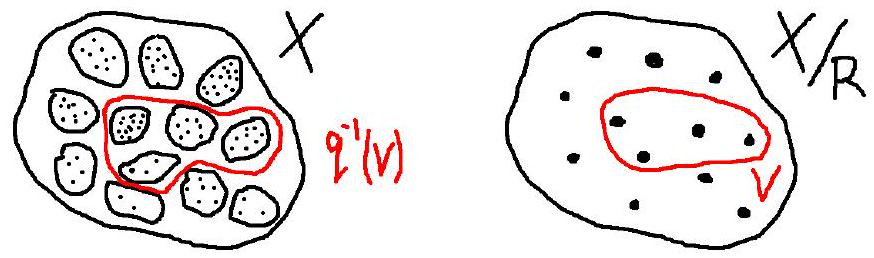
\includegraphics[scale=0.4]{at3.jpg}
\end{center}
\begin{example}
\begin{enumerate}
  \item $\mathbb{R}$ in the usual topology is also an abelian group under addition. Then $\mathbb{Z} \leqslant \mathbb{R}$ and we can form the quotient group $\mathbb{R} / \mathbb{Z}$, which is an example of a quotient space with relation $x \sim y \Longleftrightarrow x-y \in \mathbb{Z}$. Elements of $[0,1]$ represent different cosets except for $0+\mathbb{Z}=1+\mathbb{Z}$ : in the quotient space, 0 and 1 are "glued together". There are no other cosets, so the quotient space $\mathbb{R} / \mathbb{Z}$ is a circle. More precisely, $\mathbb{R} / \mathbb{Z}$ in the quotient topology is homeomorphic to a circle. This is not obvious.

  \item This time consider the quotient group $\mathbb{R} / \mathbb{Q}$. The quotient map $q: \mathbb{R} \rightarrow \mathbb{R} / \mathbb{Q}$ is a group homomorphism. Assume that $V \subset \mathbb{R} / \mathbb{Q}$ is open and non-empty. Then $q^{-1}(V)$ is a non-empty open subset of $\mathbb{R}$, and hence $(a, b) \subset q^{-1}(V)$ for some $a<b$ in $\mathbb{R}$. Given $x \in \mathbb{R}$, there exists $r \in \mathbb{Q} \cap(a-x, b-x)$. It follows that $x+r \in(a, b)$, and hence $q(x)=q(x+r) \in V$ and $x \in q^{-1}(V)$. We have shown that $q^{-1}(V)=\mathbb{R}$, and thus $V=q\left(q^{-1}(V)\right)=\mathbb{R} / \mathbb{Q}$. The quotient topology is the indiscrete topology! So a quotient of a metrizable space need not be metrizable.
\item Consider the unit square $Q=[0,1] \times[0,1]$ in $\mathbb{R}^{2}$ with the following equivalence relation:
$$
(x, y) \sim\left(x^{\prime}, y^{\prime}\right) \Longleftrightarrow \begin{cases}(x, y)=\left(x^{\prime}, y^{\prime}\right) & \text { or } \\ x=x^{\prime},\left\{y, y^{\prime}\right\}=\{0,1\} & \text { or } \\ \left\{x, x^{\prime}\right\}=\{0,1\}, y=y^{\prime} & \end{cases}
$$
\begin{center}
    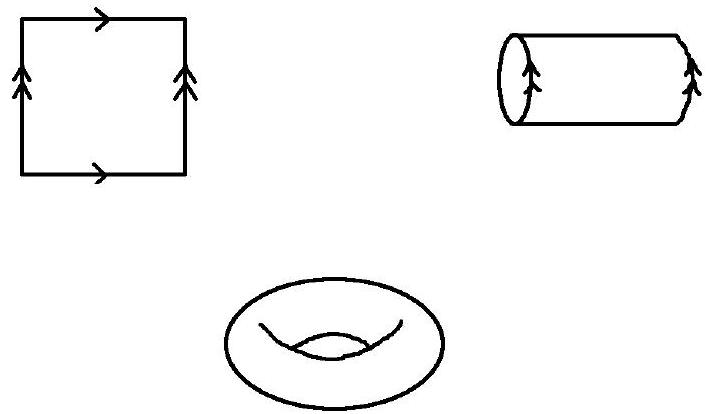
\includegraphics[scale=0.4]{at4.jpg}
\end{center}
The space \( Q / R \) is homeomorphic to \( \mathbb R^2 / \mathbb Z^2 \).
	This is a square where the top and bottom edges are identified as the same, and the left and right edges are also identified as the same.
	This is homeomorphic to the surface of a torus with the Euclidean topology embedded in Euclidean three-dimensional space.
\end{enumerate}
\end{example}

\paragraph{Recall from IA Numbers and Sets }
Let $X$ be a set and $R$ be an equivalence relation on $X$. Let $q: X \rightarrow X / R$ be the quotient map.

Suppose $Y$ is another set and a function $f: X \rightarrow Y$ \textbf{respects} the relation $R$ :
$$
\forall x, y \in X \quad x \sim y \Longrightarrow f(x)=f(y)
$$

Then there is a unique function $\tilde{f}: X / R \rightarrow Y$ such that $f=\tilde{f} \circ q$. So the following diagram commutes. 
\begin{center}
\begin{tikzcd}
    X \arrow[r,"f"] \arrow[d,"q"] & Y\\ 
    X/R \arrow[ur, "\tilde{f}"] & 
\end{tikzcd}
\end{center}
\begin{proof}
    given $z \in X / R$, write $z=q(x)$ for some $x \in X$, then set $\tilde{f}(z)=f(x)$.
\end{proof}

\begin{note}
    \begin{enumerate}
        \item $\operatorname{im}(f)=\operatorname{im}(\tilde{f})$ So $f$ surjective $\Longrightarrow \tilde{f}$ surjective.
      
        \item Suppose $f$ \textbf{fully respects} $R: \forall x, y \in X \quad x \sim y \Longleftrightarrow f(x)=f(y)$
        
        Then $\tilde{f}$ is injective.
      \end{enumerate}
\end{note}

\begin{proposition}\label{prop:4.10}
    Let $X, Y$ be topological spaces, let $R$ be an equivalence relation on $X$ and let $q: X \rightarrow X / R$ be the quotient map. Let $f: X \rightarrow Y$ be a function that respects the relation $R$. Then the following hold.
    \begin{enumerate}[(i)]
        \item If $f$ is continuous, then $\tilde{f}$ is continuous.

        \item If $f$ is an open map, then $\tilde{f}$ is an open map.
    \end{enumerate}
    (Here $\tilde{f}: X / R \rightarrow Y$ is the unique map with $\tilde{f} \circ q=f$.) In particular, if $f$ is continuous, surjective and fully respects $R$, then $\tilde{f}$ is a continuous bijection. If in addition, $f$ is an open map, then $\tilde{f}$ is a homeomorphism.
\end{proposition}
\begin{proof}
    (i) Let $V$ be an open subset of $Y$. Is $\tilde{f}^{-1}(V)$ open in $X / R$ ? We have $q^{-1}\left(\tilde{f}^{-1}(V)\right)=(\tilde{f} \circ q)^{-1}(V)=f^{-1}(V)$, which is open in $X$ since $f$ is continuous. Hence, $\tilde{f}^{-1}(V)$ is open in $X / R$, and so $\tilde{f}$ is continuous.

    (ii) Let $V$ be an open subset of $X / R$. Then $U=q^{-1}(V)$ is open in $X$ and $q(U)=q\left(q^{-1}(V)\right)=V$. Hence, $\tilde{f}(V)=\tilde{f}(q(U))=f(U)$, which is open in $Y$. Thus, $\tilde{f}$ is open.
\end{proof}

\begin{example}
    $\mathbb{R} / \mathbb{Z}$ is homeomorphic to $S^{1}=\left\{x \in \mathbb{R}^{2}:\|x\|=1\right\}$.

    Define $f: \mathbb{R} \rightarrow S^{1}$ by $f(t)=(\cos (2 \pi t), \sin (2 \pi t))$. Then $f$ is continuous, surjective and for $s, t \in \mathbb{R}$, we have $s-t \in \mathbb{Z} \Longleftrightarrow f(s)=f(t)$. So by Proposition \ref{prop:4.10}, there is a unique map $\tilde{f}: \mathbb{R} / \mathbb{Z} \rightarrow S^{1}$ with $f=\tilde{f} \circ q$, and moreover, $\tilde{f}$ is a continuous bijection.

    It remains to check that $f$ is an open map. 
    \begin{itemize}
        \item Let $U$ be an open subset of $\mathbb{R}$, and assume for a contradiction that $f(U)$ is not open in $S^{1}$. 
        \item Then its complement is not closed, so it contains a sequence $\left(z_{n}\right)$ that converges to some $z \in f(U)$. 
        \item For each $n \in \mathbb{N}$ choose $x_{n} \in[0,1]$ such that $z_{n}=f\left(x_{n}\right)$. This can be done since $f$ is surjective.  
        \item Note that $x_{n} \notin U$ since $z_{n} \notin f(U)$. After passing to a subsequence, we may assume that $x_{n} \rightarrow x$ for some $x \in[0,1]$ (Bolzano-Weierstrass). 
        \item Then $f\left(x_{n}\right) \rightarrow f(x)$ by continuity, and so $f(x)=z$. 
        \item Since $z \in f(U)$, we have $z=f(y)$ for some $y \in U$. Then $k=y-x \in \mathbb{Z}$. 
        \item Now $f\left(x_{n}+k\right)=f\left(x_{n}\right)=z_{n} \notin f(U)$, and thus $x_{n}+k \notin U$. On the other hand, $x_{n}+k \rightarrow x+k=y$. Since $\mathbb{R} \setminus U$ is closed, we have $y \notin U$, a contradiction.
    \end{itemize}

    Later we will have a much better way of proving that $f$ is open.
\end{example}

\begin{proposition}
    Let $X$ be a topological space and $R$ an equivalence relation on $X$.
    \begin{enumerate}[(a)]
        \item If $X / R$ Hausdorff, then $R$ is closed in $X \times X$.
        \item If $R$ is closed in $X \times X$ and $q: X \rightarrow X / R$ is open, then $X / R$ is Hausdorff.
    \end{enumerate}
\end{proposition}

\begin{proof}
    (a) Given $(x, y) \in X \times X \setminus R$, we have $x \not\sim y$, so $q(x) \neq q(y)$. Thus, there exist disjoint open sets $S, T$ in $X / R$ such that $q(x) \in S$ and $q(y) \in T$. Then $U=q^{-1}(S)$ and $V=q^{-1}(T)$ are disjoint open sets in $X$ with $x \in U$ and $y \in V$. 
    
    Now for all $a \in U$ and $b \in V$, we have $q(a) \in S$ and $q(b) \in T$, and so $a \not\sim b$, i.e., $(a, b) \notin R$. It follows that $(x, y) \in U \times V \subset X \times X \setminus R$. This proves that $R$ has open complement, and thus $R$ is closed.

(b) Given $z \neq w$ in $X / R$, choose $x, y \in X$ with $z=q(x)$ and $w=q(y)$. Then $(x, y) \notin R$, i.e., the open set $X \times X \setminus R$ contains $(x, y)$. Thus, there exist open set $U, V$ in $X$ such that $(x, y) \in U \times V \subset X \times X \setminus R$. 

Since $q$ is an open map, $q(U)$ and $q(V)$ are open sets in $X / R$ with $z=q(x) \in q(U)$ and $w=q(y) \in q(V)$. Finally, $q(U) \cap q(V)=\emptyset$ since otherwise, there exist $a \in U$ and $b \in V$ with $q(a)=q(b)$, and thus $(a, b) \in R \cap U \times V$, contradicting the choice of $U, V$.
\end{proof}

\section{Connectedness}
\subsection{Definition}

Recall the Intermediate Value Theorem (IVT): Let $f: I \rightarrow \mathbb{R}$ be a continuous function on the interval $I$. Given $x<y$ in $I$ and $c \in \mathbb{R}$ strictly between $f(x)$ and $f(y)$, there exists $z \in(x, y)$ such that $f(z)=c$.

A subset $I$ of $\mathbb{R}$ is an interval if the following holds: for all $x, y, z \in \mathbb{R}$ if $x<y<z$ and $x, z \in I$, then $y \in I$. So the IVT says that the continunous image of an interval is an interval.

\begin{sque}
    For what topological spaces does the IVT hold?
\end{sque}

\begin{example}
    The function
    $$
    f: X=[0,1) \cup(1,2] \rightarrow \mathbb{R} \quad x \mapsto \begin{cases}0 & \text { if } x \in[0,1) \\ 1 & \text { if } x \in(1,2]\end{cases}
    $$
    is continuous but its image is not an interval.
\end{example}

\begin{definition}
    A topological space $X$ is \textbf{disconnected} if there exist subsets $U$ and $V$ of $X$ such that

    \begin{enumerate}[(i)]
    \item $U \neq \emptyset$ and $V \neq \emptyset$

    \item $U$ and $V$ are open in $X$

    \item $U \cap V=\emptyset$

    \item $U \cup V=X$

    \end{enumerate}

    In this case, we say that the subsets $U$ and $V$ of $X$ \textbf{disconnect} $X$.

    We say $X$ is \textbf{connected} if $X$ is not disconnected.
\end{definition}

\begin{theorem}\label{thm:connected tfae}
    For a topological space $X$ the followings are equivalent.
    \begin{enumerate}[(i)]
        \item $X$ is connected.
        \item $f: X \rightarrow \mathbb{R}$ continuous $\Longrightarrow f(X)$ is an interval.
        \item $f: X \rightarrow \mathbb{Z}$ continuous $\Longrightarrow f$ is constant.
    \end{enumerate}
\end{theorem}

\begin{proof}
    ((i) $ \Rightarrow$ (ii)) Suppose $f: X \rightarrow \mathbb{R}$ is continuous but $f(X)$ is not an interval. So there exists $a<b<c$ in $\mathbb{R}$ with $a, c \in f(X)$ and $b \notin f(X)$. Choose $x, z \in X$ with $f(x)=a$ and $f(z)=c$. 
    
    We show that $U=f^{-1}(-\infty, b)$ and $V=f^{-1}(b, \infty)$ disconnect $X$, which will contradict (i). Indeed, $U$ and $V$ are non-empty ($x \in U$ and $z \in V$), open (as $f$ is continuous), disjoint and $U \cup V=X$ since $b \notin f(X)$.

    ((ii) $\Rightarrow$ (iii)) The inclusion map $\iota: \mathbb{Z} \rightarrow \mathbb{R}$ is continuous. So if $f: X \rightarrow \mathbb{Z}$ is continuous, then so is $g=\iota \circ f: X \rightarrow \mathbb{R}$. Then $g(X)$ is an interval by (ii) but at the same time $g(X)=f(X) \subset \mathbb{Z}$. So $f$ must have been constant.
 
    ((iii) $\Rightarrow$ (i)) Assume that $U$ and $V$ disconnect $X$. Define
    $$
    f: x \rightarrow \mathbb{Z} \quad x \mapsto \begin{cases}0 & \text { if } x \in U \\ 1 & \text { if } x \in V\end{cases}
    $$
    Then for any $A \subset \mathbb{Z}$, we have $f^{-1}(A)$ is one of $\emptyset, U, V$ or $X$ depending on whether $A \cap\{0,1\}$ is $\emptyset,\{0\},\{1\}$ or $\{0,1\}$, respectively. Thus, $f$ is continuous but not constant as $U$ and $V$ are non-empty.
\end{proof}

\begin{corollary}
    Let $X \subset \mathbb{R}$. Then $X$ is connected $\Longleftrightarrow X$ is an interval.
\end{corollary}
\begin{proof}
    ($ \Rightarrow $) The inclusion map $\iota: X \rightarrow \mathbb{R}$ is continuous, so its image $X$ is an interval. 
    
    Alternatively, if $X$ is not an interval, then there exist $a<b<c$ in $\mathbb{R}$ with $a, c \in X$ and $b \notin X$. It follows that $U=(-\infty, b) \cap X$ and $V=(b, \infty) \cap X$ disconnect $X$.

    ($ \Leftarrow $) Suppose $X$ is an interval. By IVT and the previous theorem, $X$ is connected. 
    
    Alternatively, assume $U$ and $V$ disconnect $X$. Fix $x \in U$ and $y \in V$. Assume wlog $x<y$. Let $z=\sup (U \cap[x, y])$. Then $z \in[x, y] \subset X$. We show that $z \in U \cap V$. 
    
    For each $n \in \mathbb{N}$, there exists $x_{n} \in U \cap[x, y]$ with $z-\frac{1}{n}<x_{n} \leqslant z$. Then $x_{n} \rightarrow z$, and hence $z \in U$ as $U=X \setminus V$ is closed in $X$. It follows that $z<y$ (otherwise $z \in V$ and we are done). Hence for large $n$, we have $z+\frac{1}{n} \in[x, y]$ and so $z+\frac{1}{n} \in V$. Since $V=X \setminus U$ is closed in $X$, it follows that $z \in V$.
\end{proof}

\subsection{Consequences of definition}\ \vspace{-1.5em}

\begin{example}
    \begin{enumerate}
        \item Any indiscrete space is connected.
      
        \item The cofinite topology on an infinite set is connected.
      
        \item The discrete topology on a set $X$ of size at least 2 is disconnected. Indeed, for any $x \in X$, the subsets $\{x\}$ and $X \setminus\{x\}$ disconnect $X$.
      
      \end{enumerate}
\end{example}

\begin{lemma}
    Let $Y$ be a subspace of a topological space $X$. Then $Y$ is disconnected if and only if there exist open subsets $U$ and $V$ of $X$ such that $U \cap Y \neq \emptyset$, $V \cap Y \neq \emptyset, U \cap V \cap Y=\emptyset$ and $Y \subset U \cup V$.
\end{lemma}
\begin{proof}
    ($ \Rightarrow $) Let subsets $U^{\prime}$ and $V^{\prime}$ of $Y$ disconnect $Y$. By definition of the subspace topology, there are open sets $U$ and $V$ in $X$ such that $U^{\prime}=U \cap Y$ and $V^{\prime}=V \cap Y$. Then $U \cap Y=U^{\prime} \neq \emptyset, V \cap Y=V^{\prime} \neq \emptyset$, $U \cap V \cap Y=U^{\prime} \cap V^{\prime}=\emptyset$ and $Y=U^{\prime} \cup V^{\prime} \subset U \cup V$.

    ($ \Leftarrow $) Now assume that $U$ and $V$ are open subsets of $X$ such that $U \cap Y \neq \emptyset, V \cap Y \neq \emptyset, U \cap V \cap Y=\emptyset$ and $Y \subset U \cup V$. Then $U^{\prime}=U \cap Y$ and $V^{\prime}=V \cap Y$ disconnect $Y$.
\end{proof}

\begin{note}
    If $Y$ is a subspace of $X$, and $U$ and $V$ are open subsets of $X$ such that $U \cap Y \neq \emptyset, V \cap Y \neq \emptyset, U \cap V \cap Y=\emptyset$ and $Y \subset U \cup V$, then we will say that the open subsets $U, V$ of $X$ disconnect $Y$.
\end{note}

\begin{proposition}\label{prop:closure connected}
    Let $Y$ be a subspace of a topological space $X$. If $Y$ is connected, then its closure $\bar{Y}$ in $X$ is also connected.
\end{proposition}
\begin{proof}
    Assume $\bar{Y}$ is disconnected. Then there are open subsets $U, V$ in $X$ such that $U \cap \bar{Y} \neq \emptyset, V \cap \bar{Y} \neq \emptyset, U \cap V \cap \bar{Y}=\emptyset$ and $\bar{Y} \subset U \cup V$. Then $U \cap V \cap Y=\emptyset$ and $Y \subset U \cup V$.

    If in addition, we also have $U \cap Y \neq \emptyset$ and $V \cap Y \neq \emptyset$, then $Y$ is disconnected by lemma. So one of $U \cap Y$ and $V \cap Y$ must be empty. Wlog $U \cap Y=\emptyset$, and so $Y$ is a subset of the closed set $X \setminus U$. It follows that $\bar{Y} \subset X \setminus U$ contradicting $U \cap \bar{Y} \neq \emptyset$.
\end{proof}

\begin{remark}
    \begin{enumerate}
        \item More generally, if $Y$ is connected and $Y \subset Z \subset \bar{Y}$, then $Z$ is connected. Indeed, the closure of $Y$ in $Z$ is $\bar{Y} \cap Z$ (Proposition \ref{prop:4.6}).
      
        \item An alternative proof of Proposition \ref{prop:closure connected} is via Theorem \ref{thm:connected tfae} (iii).
      
      \end{enumerate}
\end{remark}

\begin{theorem}\label{thm:continuous image connected}
    Let $f: X \rightarrow Y$ be a continuous function. If $X$ is connected, then $f(X)$ is also connected. (The continuous image of a connected space is connected.)
\end{theorem}

\begin{proof}
    Assume that $U, V$ are open subsets of $Y$ that disconnect $f(X)$.

    Then $f^{-1}(U)$ and $f^{-1}(V)$ are open in $X$ since $f$ is continuous.

    $f^{-1}(U)$ is non-empty since $U \cap f(X) \neq \emptyset$, and similarly $f^{-1}(V)$ is non-empty.

    If $x \in f^{-1}(U) \cap f^{-1}(V)$, then $f(x) \in U \cap V \cap f(X)=\emptyset$. This contradiction shows that $f^{-1}(U) \cap f^{-1}(V)=\emptyset$.

    Finally, $f^{-1}(U) \cup f^{-1}(V)=f^{-1}(U \cup V)=X$ since $U \cup V \supset f(X)$.

    So $f^{-1}(U)$ and $f^{-1}(V)$ disconnect $X$ contradicting the assumption that $X$ is connected.
\end{proof}

\begin{remark}
    \begin{enumerate}
        \item Connectedness is a topological property.
      
        \item If $f: X \rightarrow Y$ is a continuous function and $A \subset X$ is a connected subset of $X$, then $f(A)$ is connected. Apply Theorem \ref{thm:continuous image connected} to $f\restriction_{A}: A \rightarrow Y$.
      \end{enumerate}
\end{remark}

Since the quotient map is continuous, we get
\begin{corollary}
    The quotient space of a connected space is connected.
\end{corollary}

\begin{example}
    Consider the subset $Y=\left\{\left(x, \sin \frac{1}{x}\right): x>0\right\}$ of $\mathbb{R}^{2}$. 
    
    The function $f:(0, \infty) \rightarrow \mathbb{R}^{2}, x \mapsto\left(x, \sin \frac{1}{x}\right)$, is continuous, and hence its image $Y$ is connected. It follows that $\bar{Y}$ is also connected. Note that
    $$
    \bar{Y}=Y \cup\{(0, y):-1 \leqslant y \leqslant 1\}
    $$
    Indeed, let $-1 \leqslant y \leqslant 1$. For $n \in \mathbb{N}$, the function $x \mapsto \frac{1}{x} \operatorname{maps}\left(0, \frac{1}{n}\right)$ onto $(n, \infty)$, and hence sin $\frac{1}{x_{n}}=y$ for some $x_{n} \in\left(0, \frac{1}{n}\right)$. Then $\left(x_{n}, \sin \frac{1}{x_{n}}\right) \rightarrow(0, y)$, and hence $(0, y) \in \bar{Y}$. This shows that $\widetilde{Y}=Y \cup\{(0, y):-1 \leqslant y \leqslant 1\}$ is contained in $\bar{Y}$. 
    
    Conversely, $\bar{Y} \subset \widetilde{Y}$ follows if we show that $\widetilde{Y}$ is closed. So assume $\left(x_{n}, y_{n}\right) \rightarrow(x, y)$ in $\mathbb{R}^{2}$ with $\left(x_{n}, y_{n}\right) \in \widetilde{Y}$ for all $n \in \mathbb{N}$. Since $x_{n} \geqslant 0$ and $-1 \leqslant y_{n} \leqslant 1$ for all $n$, we have $x \geqslant 0$ and $-1 \leqslant y \leqslant 1$. So if $x=0$, then $(x, y) \in \widetilde{Y}$. Otherwise, $x>0$, so $x_{n}>0$ for all large $n$. Now, if $x_{n}>0$, then $y_{n}=\sin \frac{1}{x_{n}}$. Thus, $y_{n} \rightarrow \sin \frac{1}{x}$ and $(x, y)=\left(x, \sin \frac{1}{x}\right) \in \widetilde{Y}$.
\end{example}

\begin{lemma}\label{lma:union connected}
    Let $X$ be a topological space and let $\mathcal{A}$ be a family of connected subsets of $X$. Assume that $A \cap B \neq \emptyset$ for all $A, B \in \mathcal{A}$. Then $\bigcup_{A \in \mathcal{A}} A$ is connected.
\end{lemma}

\begin{proof}
    Set $Y=\bigcup_{A \in \mathcal{A}} A$ and assume that $f: Y \rightarrow \mathbb{Z}$ is continuous. We show that $f$ must be constant. Then by Theorem \ref{thm:connected tfae} it will follow that $Y$ is connected. For each $A \in \mathcal{A}$, the restriction $f\restriction_{A}: A \rightarrow \mathbb{Z}$ is continuous, and thus constant by Theorem \ref{thm:connected tfae}. For any $A, B \in \mathcal{A}$, the functions $f\restriction_{A}$ and $f\restriction_{B}$ must take the same constant value since $A \cap B \neq \emptyset$. It follows that $f$ itself must be a constant function.
\end{proof}

\begin{theorem}\label{thm:product connected}
    Let $X$ and $Y$ be connected topological space. Then $X \times Y$ is connected in the product topology.
\end{theorem}
\begin{proof}
    Wlog $X$ and $Y$ are non-empty.

    Fix $x_{0} \in X$ and consider the map $f: Y \rightarrow X \times Y, y \mapsto\left(x_{0}, y\right)$. We show that $f$ is continuous. Given open sets $U$ in $X$ and $V$ in $Y$, if $x_{0} \in U$, then $f^{-1}(U \times V)=V$ and if $x_{0} \notin U$, then $f^{-1}(U \times V)=\emptyset$. It follows that $f$ is continuous.

    Alternatively, recall that $q_{X}: X \times Y \rightarrow X$ and $q_{Y}: X \times Y \rightarrow Y$ denote coordinate projections. Then $q X \circ f: Y \rightarrow X$ is the constant function $y \mapsto x_{0}$ and $q_{Y} \circ f: Y \rightarrow Y$ is the identity function $y \mapsto y$, and thus both are continuous. It then follows that $f$ is continuous.

    Since $Y$ is connected and $f$ is continuous, $\left\{x_{0}\right\} \times Y$, the image of $f$, is connected. Similarly, for any $y_{0} \in Y$, the subspace $X \times\left\{y_{0}\right\}$ of $X \times Y$ is connected.

    From here, we give two ways of completing the proof of the theorem. In the first method, we assume that $U$ and $V$ disconnect $X \times Y$. Fix $x_{0} \in X$. Since $\left\{x_{0}\right\} \times Y$ is connected, $U, V$ cannot disconnect $\left\{x_{0}\right\} \times Y$. Hence either $U$ or $V$ has empty intersection with $\left\{x_{0}\right\} \times Y$, and so wlog we may assume that $\left\{x_{0}\right\} \times Y \subset U$. Similarly, for any $y \in Y$, the set $X \times\{y\}$ is contained either in $U$ or in $V$, and since $\left(x_{0}, y\right) \in U$, we must in fact have $X \times\{y\} \subset U$. Thus, $X \times Y \subset U$ and $V=\emptyset$, a contradiction.

    In the second method we first observe that for $x_{0} \in X$ and $y_{0} \in Y$, the connected sets $\left\{x_{0}\right\} \times Y$ and $X \times\left\{y_{0}\right\}$ have non-empty intersection $\left\{\left(x_{0}, y_{0}\right)\right\}$. It follows by Lemma \ref{lma:union connected} that $\left\{x_{0}\right\} \times Y \cup X \times\left\{y_{0}\right\}$ is connected. Now fix $x_{0} \in X$ and for each $y \in Y$ set $A_{y}=\left\{x_{0}\right\} \times Y \cup X \times\{y\}$. For $y, y^{\prime} \in Y$, we have $A_{y} \cap A_{y^{\prime}} \supset\left\{x_{0}\right\} \times Y$, and hence $A_{y} \cap A_{y^{\prime}}$ is non-empty. Hence by Lemma \ref{lma:union connected} it follows that $\bigcup_{y \in Y} A_{y}=X \times Y$ is connected.
\end{proof}

\begin{example}
    $\mathbb{R}^{n}$ is connected for any $n \in \mathbb{N}$.
\end{example}

\begin{remark}
    \begin{enumerate}
        \item In the proof we showed that $y \mapsto(x, y)$ is a continuous map $Y \rightarrow X \times Y$ with image $\{x\} \times Y$. In fact, this map is injective with inverse $\{x\} \times Y \rightarrow Y$ being the second coordinate projection, which is continuous. It follows that $\{x\} \times Y$ is homeomorphic to $Y$ for any $x \in X$. Similarly, $X \times\{y\}$ is homeomorphic to $X$ for any $y \in Y$.
      
        \item The converse of Theorem \ref{thm:product connected} also holds provided $X$ and $Y$ are non-empty: If $X \times Y$ is connected, then so are $X$ and $Y$. Simply apply Theorem \ref{thm:continuous image connected} to the coordinate projections.
      \end{enumerate}
\end{remark}

\subsection{Components}
We define a relation $\sim$ on a topological space $X$ as follows:
$$
\forall x, y \in X \quad x \sim y \Longleftrightarrow \exists \text { connected subset } A \text { of } X \text { such that } x, y \in A
$$
We check that this is an equivalence relation. For any $x \in X$, the set $\{x\}$ is connected, and so $x \sim x$. Symmetry is immediate from the definition. Finally, if $x \sim y$ and $y \sim z$, then there exist connected subsets $A, B$ of $X$ with $x, y \in A$ and $y, z \in B$. Since $A \cap B \neq \emptyset$, it follows from Lemma \ref{lma:union connected} that $A \cup B$ is connected, and hence $x \sim z$. 
\begin{definition}
    For $x \in X$, we shall write $C_{x}$ for the equivalence class containing $x$. Equivalence classes are called \textbf{connected components} of $X$.
\end{definition}

\begin{proposition}\label{prop: connected components are maximal and partition}
    Connected components of a topological space $X$ are non-empty, maximal (with respect to inclusion) connected subsets of $X$. Connected components are closed and they partition $X$ (i.e., $X$ is the disjoint union of its connected components).
\end{proposition}
\begin{proof}
    Let $C$ be a connected component of $X$. Then $C=C_{x}$ for some $x \in X$. Thus $C \neq \emptyset$ since $x \in C$.

If $A$ is a connected subset of $X$ with $x \in A$, then $y \sim x$ for all $y \in A$, and hence $A \subset C$. It follows that if $A$ is a connected subset of $X$ with $A \supset C$, then $A=C$.

For each $y \in C$ there is a connected subset $A_{y}$ of $X$ such that $x, y \in A_{y}$. Then $A_{y} \cap A_{y^{\prime}} \neq \emptyset$ for all $y, y^{\prime} \in C$, and hence $A=\bigcup_{y \in C} A_{y}$ is connected by Lemma \ref{lma:union connected} and $A \supset C$. By above, $A=C$, and thus $C$ is connected. By Proposition \ref{prop:closure connected}, the closure $\bar{C}$ of $C$ in $X$ is also connected. Hence by the maximality of $C$, we have $C=\bar{C}$ and $C$ is closed. 

Finally, $X$ is the disjoint union of components, since in general, equivalence classes of an equivalence relation on a set partition the set.
\end{proof}

\subsection{Path connectedness}
Apart from connectedness, we have a stronger property: joining any two points with a `path'.
\begin{definition}
    Let $X$ be a topological space. For $x, y \in X$, a \textbf{path} from $x$ to $y$ in $X$ is a continuous function $\gamma:[0,1] \rightarrow X$ such that $\gamma(0)=x$ and $\gamma(1)=y$. We say that a topological space $X$ is \textbf{path-connected} if for all $x, y \in X$ there is a path from $x$ to $y$ in $X$.
\end{definition}

\begin{note}
    What we called a path is sometimes called a \textbf{continuous path}.
\end{note}

\begin{theorem}\label{thm:path connected is connected}
    Every path-connected topological space is connected.
\end{theorem}

\begin{proof}
    Assume $X$ is path-connected but not connected. Let $U, V$ disconnect $X$. Fix $x \in U, y \in V$ and a continuous function $\gamma:[0,1] \rightarrow X$ with $\gamma(0)=x$ and $\gamma(1)=y$. It is straightforward to check that $\gamma^{-1}(U)$ and $\gamma^{-1}(V)$ disconnect $[0,1]$ contradicting that $[0,1]$ is connected.
\end{proof}
The converse of above is FALSE.
\begin{example}
    Recall that the subset
    \[
        X=\left\{\left(x, \sin \frac{1}{x}\right): x>0\right\} \cup\{(0, y):-1 \leqslant y \leqslant 1\}
    \]
    of $\mathbb{R}^{2}$ is connected. We now show that $X$ is not path-connected.

    Assume $\gamma:[0,1] \rightarrow X$ is continuous with $\gamma(0)=(0,0)$ and $\gamma(1)=(1, \sin 1)$.

    Let $\gamma_{1}$ and $\gamma_{2}$ be the components of $\gamma$. So $\gamma(t)=\left(\gamma_{1}(t), \gamma_{2}(t)\right)$ for all $t \in[0,1]$. Since $\gamma$ is continuous, so are $\gamma_{1}$ and $\gamma_{2}$.

    Assume that $x=\gamma_{1}(t)>0$ for some $t$ (e.g., this is true for $t=1$). By the IVT, the image of $(0, t)$ under $\gamma_{1}$ contains $(0, x)$. Choose $n \in \mathbb{N}$ such that $\frac{1}{2 \pi n} \in(0, x)$ and $s \in(0, t)$ such that $\gamma_{1}(s)=\frac{1}{2 \pi n}$. Then $\gamma_{2}(s)=\sin \frac{1}{\gamma_{1}(s)}=0$. Similarly, there exists $s \in(0, t)$ with $\gamma_{1}(s)=\frac{1}{2 \pi n+\frac{\pi}{2}}$ and $\gamma_{2}(s)=1$. 
    
    We now inductively construct $t_{1}>t_{2}>\cdots>0$ in $[0,1]$ such that $\gamma_{2}\left(t_{n}\right)=0$ if $n$ is even and $\gamma_{2}\left(t_{n}\right)=1$ otherwise. 
    Let $t_1$ be such that $ \gamma_1(t_1) = \frac{1}{2\pi n} $. We can find $ t_2 \in (0,t_1) $ such that $ \gamma_1(t_2) =\frac{1}{2\pi n+\frac{\pi}{2} } $ and $\gamma_2(t_2)=0$. This process continues inductively.
    
    Let $t_{n} \rightarrow t$ in $[0,1]$. Then $\gamma_{2}\left(t_{n}\right) \rightarrow \gamma_{2}(t)$. However, $\left(\gamma_{2}\left(t_{n}\right)\right)$ is not convergent --- a contradiction.
\end{example}

\begin{lemma}[Gluing lemma]\label{lma:Gluing lemma}
    Let $X$ be a topological space and let $A, B$ be closed subsets with $X=A \cup B$. If $f: X \rightarrow Y$ is a function such that $f\restriction_{A}: A \rightarrow Y$ and $f\restriction_{B}: B \rightarrow Y$ are continuous, then $f$ is continuous.
\end{lemma}

\begin{proof}
    Let $V$ be a closed subset of $Y$. Since $f\restriction_{A}$ is continuous, it follows that $\left(f\restriction_{A}\right)^{-1}(V)=A \cap f^{-1}(V)$ is closed in $A$, and hence also in $X$ (Proposition \ref{prop:4.6}). Similarly, $B \cap f^{-1}(V)$ is closed in $X$. It follows that

$$
f^{-1}(V)=\left(A \cap f^{-1}(V)\right) \cup\left(B \cap f^{-1}(V)\right)
$$

is also closed in $X$. Finally, $f$ is continuous by Proposition \ref{prop:4.8} (i).
\end{proof}

\subsection{Path-connected components}
Similar to connected components, we have path-connected components.

Let $X$ be a topological space. We define a relation on $X$ as follows.
$$
\forall x, y \in X \quad x \sim y \Longleftrightarrow \exists \text { path from } x \text { to } y \text { in } X
$$
For $x \in X$, the constant function with value $x$ is continuous, which shows that $x \sim x$. 

If $\gamma$ is a path from $x$ to $y$, then $t \mapsto \gamma(1-t)$ is a path from $y$ to $x$, which shows symmetry. 

Finally, if $\gamma$ is a path from $x$ to $y$ and $\delta$ is a path from $y$ to $z$, then
$$
\eta(t)= \begin{cases}\gamma(2 t) & \text { if } t \in\left[0, \frac{1}{2}\right] \\ \delta(2 t-1) & \text { if } t \in\left[\frac{1}{2}, 1\right]\end{cases}
$$
defines a path from $x$ to $z$. Indeed, firstly this well-defined at $\frac{1}{2}$ since
$\gamma(1)=\delta(0)=y$. Secondly, the sets $\left[0, \frac{1}{2}\right]$ and $\left[\frac{1}{2}, 1\right]$ are closed in $[0,1]$, $[0,1]=\left[0, \frac{1}{2}\right] \cup\left[\frac{1}{2}, 1\right]$ and the functions $\eta\restriction_{\left[0, \frac{1}{2}\right]}, \eta \restriction_{\left[\frac{1}{2}, 1\right]}$ are continuous. So $\eta$ is continuous by Lemma \ref{lma:Gluing lemma}. This shows that $\sim$ is transitive.

\begin{definition}
    Equivalence classes of this relation are called \textbf{path-connected components} of $X$. 
\end{definition}
\begin{note}
    It is immediate from the fact that $\sim$ is an equivalence relation that path-connected components are path-connected.
\end{note}

\begin{theorem}\label{thm:Rn connected iff path-connected}
    An open subset $U$ of $\mathbb{R}^{n}$ is connected $\Longleftrightarrow$ path-connected.
\end{theorem}
\begin{proof}
    $(\Longleftarrow)$ This is true in general by Theorem \ref{thm:path connected is connected}.

$(\Longrightarrow)$ Fix $x_{0} \in U$ and set $P=\left\{x \in U: \exists\right.$ path from $x_{0}$ to $\left.x\right\}$. In other words, $P$ is the path-connected component of $x_{0}$ in $U$. We show that $P$ is both open and closed in $U$. (Such a set is called \textbf{clopen}.) Since $P$ and $U \setminus P$ cannot disconnect $U$, one of them has to be empty. Since $x_{0} \in P$, it follows that $P=U$, and thus $U$ is path-connected.

Fix $x \in P$. Since $U$ is open, there exists $r>0$ such that $D_{r}(x) \subset U$. Now, for any $y \in D_{r}(x)$, there is a path from $x$ to $y$ inside $D_{r}(x)$ (and hence inside $U$ ). For example, the straight line segment $t \mapsto(1-t) x+t y$ is continuous and takes values in $D_{r}(x):\|((1-t) x+t y)-x\|=\|t(y-x)\|=t\|y-x\|<r$ This shows that $D_{r}(x) \subset P$, and thus $P$ is open in $U$.

Now fix $x \in U \setminus P$ and again choose $r>0$ such that $D_{r}(x) \subset U$. As before, for any $y \in D_{r}(x)$, we have $y \sim x$. Hence, if there exists $y \in D_{r}(x) \cap P$, then $y \sim x$ and $y \sim x_{0}$, which gives the contradiction $x \in P$. It follows that $D_{r}(x) \subset U \setminus P$, and thus $U \setminus P$ is open in $U$.
\end{proof}

\subsection{An application of connectedness}
By considering connectedness, we can show that
\begin{theorem}\label{th,:R, Rn not homeo}
    For $n \geqslant 2, \mathbb{R}$ and $\mathbb{R}^{n}$ are not homeomorphic.
\end{theorem}

\begin{proof}
    Assume that $f: \mathbb{R} \rightarrow \mathbb{R}^{n}$ is a homeomorphism with inverse $g: \mathbb{R}^{n} \rightarrow \mathbb{R}$. Then $f\restriction_{\mathbb{R} \setminus\{0\}}$ is a continuous bijection from $\mathbb{R} \setminus\{0\}$ onto $\mathbb{R}^{n} \setminus\{f(0)\}$ whose inverse is $g\restriction_{\mathbb{R}^{n} \setminus\{f(0)\}}$ which is also continuous. Thus, $\mathbb{R} \setminus\{0\}$ and $\mathbb{R}^{n} \setminus\{f(0)\}$ are homeomorphic. Now, $\mathbb{R} \setminus\{0\}$ is not connected since it is not an interval. However, it is easy to see that $\mathbb{R}^{n} \setminus\{f(0)\}$ is path-connected, and hence connected. Since connectedness is a topological property, we have reached the desired contradiction.
\end{proof}

\section{Compactness}
\subsection{Definition and motivation of compactness}
Recall that a continuous real-valued function on a closed bounded interval is bounded and attains its bounds.

\begin{sque}
    For which topological spaces $X$ is it true that every continuous function $X \rightarrow \mathbb{R}$ is bounded?
\end{sque}

Some answers:

\begin{enumerate}
  \item For finite spaces.

  \item For spaces $X$ with the following property:

  For every continuous function $f: X \rightarrow \mathbb{R}$ there exist $n \in \mathbb{N}$ and subsets $A_{1}, \ldots, A_{n}$ of $X$ such that $X=\bigcup_{k=1}^{n} A_{k}$ and $f$ is bounded on each $A_{k}$.
\end{enumerate}

\begin{note}
    Let $X$ be a topological space and $f: X \rightarrow \mathbb{R}$ continuous. For $x \in X$ let $U_{x}=f^{-1}(f(x)-1, f(x)+1)$. Then $U_{x}$ is open, $x \in U_{x}$ and for every $y \in U_{x}$ we have
    $$
    |f(y)| \leqslant|f(y)-f(x)|+|f(x)| \leqslant|f(x)|+1
    $$
    So $X=\bigcup_{x \in X} U_{x}$ and $f$ is bounded on each $U_{x}$. If there exists a finite set $F \subset X$ such that $X=\bigcup_{x \in F} U_{x}$, then $f$ is bounded.
\end{note}

\begin{definition}
    Let $X$ be a topological space.

    An \textbf{open cover} for $X$ is a family $\mathcal{U}$ of open subsets of $X$ such that $\bigcup_{U \in \mathcal{U}} U=X$.

    A \textbf{subcover} of an open $\operatorname{cover} \mathcal{U}$ for $X$ is a subfamily $\mathcal{V} \subset \mathcal{U}$ such that
    $\bigcup_{U \in \mathcal{V}} U=X$. If $\mathcal{V}$ is finite, then we call this a \textbf{finite subcover} of $\mathcal{U}$.

    A topological space is \textbf{compact} if every open cover for $X$ has a finite subcover.
\end{definition}

\begin{theorem}\label{thm:continuous on compact -> bounded}
    Let $X$ be a compact topological space and $f: X \rightarrow \mathbb{R}$ a continuous function.
Then $f$ is bounded, and moreover, if $X \neq \emptyset$, then $f$ attains its bounds.
\end{theorem}
\begin{proof}
    The proof of boundedness was essentially given in the Note above. Here is another proof.

    For $n \in \mathbb{N}$ let $U_{n}=\{x \in X:|f(x)|<n\}$. Then $U_{n}=f^{-1}(-n, n)$ is open in $X$.

    For every $x \in X$ there exists $n \in \mathbb{N}$ with $|f(x)|<n$. It follows that
    $X=\bigcup_{n \in \mathbb{N}} U_{n}$. Since $X$ is compact, there is a finite $F \subset \mathbb{N}$ with
    $X=\bigcup_{n \in F} U_{n}=U_{N}$ where $N=\max F$. So $f$ is bounded by $N$.

    Next, we let $m=\inf _{X} f$ and $M=\sup _{X} f$. Assume that there is no $y \in X$ with $f(y)=m$. Then for every $y \in X$ we have $f(y)>m$. Let $y \in X$. Choose $\alpha_{y} \in \mathbb{R}$ with $m<\alpha_{y}<f(y)$ and set $U_{y}=f^{-1}\left(\alpha_{y}, \infty\right)$. Then $U_{y}$ is open, it contains $y$ and $f$ is bounded below by $\alpha_{y}$ on $U_{y}$. In particular, $\left\{U_{y}: y \in X\right\}$ is an open cover for $X$. Hence there is a finite $F \subset X$ such that $X=\bigcup_{y \in F} U_{y}$. Let $\alpha=\min \left\{\alpha_{y}: y \in F\right\}$. Then $\alpha>m$ and $f$ is bounded below by $\alpha$ on $X$. This contradiction shows that $m=f(y)$ for some $y \in X$. A similar argument shows that $M$ is also attained.
\end{proof}

\begin{remark}
    Compactness is the next best thing after finiteness.
\end{remark}

\subsection{Compactness of subspaces}
Let $X$ be a topological space. We are interested in whether a subspace of $X$ is compact or not.
\begin{lemma}\label{lma:compactness of subspaces}
    Let $Y$ be a subspace of a topological space $X$. Then $Y$ is compact $\Longleftrightarrow$ for any family $\mathcal{U}$ of open subsets of $X$ satisfying $Y \subset \bigcup_{U \in \mathcal{U}} U$, there is a finite subfamily $\mathcal{V} \subset \mathcal{U}$ such that $Y \subset \bigcup_{U \in \mathcal{V}} U$.
\end{lemma}
\begin{proof}
    ($\Longrightarrow $) Let $\mathcal{U}$ be a family of open subsets of $X$ satisfying $Y \subset \bigcup_{U \in \mathcal{U}} U$. Then $\{U \cap Y: U \in \mathcal{U}\}$ is an open cover for $Y$. Since $Y$ is compact, there is a finite subcover: there is a finite $\mathcal{V} \subset \mathcal{U}$ such that $Y=\bigcup_{\mathcal{U} \in \mathcal{V}} U \cap Y$. It follows that $Y \subset \bigcup_{U \in \mathcal{V}} U$

    ($\Longleftarrow$) Let $\mathcal{W}$ be an open cover for $Y$. For each $W \in \mathcal{W}$ fix an open set $\widetilde{W}$ in $X$ such that $W=\widetilde{W} \cap Y$. Then $\mathcal{U}=\{\widetilde{W}: W \in \mathcal{W}\}$ is a family of open subsets of $X$ satisfying $Y \subset \bigcup_{U \in \mathcal{U}} U$. By assumption, there is a finite subfamily of $\mathcal{U}$ whose union still contains $Y$. So there is a finite $\mathcal{V} \subset \mathcal{W}$ such that $\bigcup_{W \in \mathcal{V}} \widetilde{W} \supset Y$. It follows that $\bigcup_{W \in \mathcal{V}} W=Y$, i.e., $\mathcal{V}$ is a finite subcover of $\mathcal{W}$.
\end{proof}

\begin{theorem}\label{lma:[0,1] is compact}
    The unit interval $[0,1]$ is compact.
\end{theorem}
\begin{proof}
    Let $\mathcal{U}$ be a family of open subsets of $\mathbb{R}$ such that $[0,1] \subset \bigcup_{U \in \mathcal{U}} U$.
    For $I \subset[0,1]$, we will say that $\mathcal{U}$ \textbf{finitely covers} $I$ if there is a finite subfamily
    $\mathcal{V} \subset \mathcal{U}$ saitsfying $I \subset \bigcup_{U \in \mathcal{V}} U$.

    We now make an observation. Suppose $I=J \cup K$ for subsets $I, J, K$ of $[0,1]$.
    If $\mathcal{U}$ finitely covers $J$ and $K$, then $\mathcal{U}$ finitely covers $I$.

    Now assume that $\mathcal{U}$ does not finitely cover $[0,1]$. Then at least one of the intervals $\left[0, \frac{1}{2}\right]$ and $\left[\frac{1}{2}, 1\right]$ cannot be finitely covered by $\mathcal{U}$. Call that interval  $[a_{1}, b_{1}]$. It follows that, putting $c=\frac{1}{2}\left(a_{1}+b_{1}\right)$, at least one of the intervals $\left[a_{1}, c\right]$ and $\left[c, b_{1}\right]$ cannot be finitely covered by $\mathcal{U}$. Call that interval $\left[a_{2}, b_{2}\right]$. Continue inductively and obtain a nested sequence
    $$
    [0,1] \supset\left[a_{1}, b_{1}\right] \supset\left[a_{2}, b_{2}\right] \supset \ldots
    $$
    such that for each $n \in \mathbb{N}$ the interval $\left[a_{n}, b_{n}\right]$ cannot be finitely covered by $\mathcal{U}$ and $b_{n}-a_{n}=2^{-n}$.

    Since $\left(a_{n}\right)$ is an increasing, bounded above sequence, it converges to some $x \in[0,1]$. Then $b_{n}=a_{n}+2^{-n} \rightarrow x$ as well.

    Since $[0,1] \subset \bigcup_{U \in \mathcal{U}} U$, there exists $U \in \mathcal{U}$ such that $x \in U$. Since $U$ is open, there exists $\varepsilon>0$ such that $(x-\varepsilon, x+\varepsilon) \subset U$. Since $a_{n}, b_{n} \rightarrow x$ there exists an $n \in \mathbb{N}$ with $a_{n}, b_{n} \in(x-\varepsilon, x+\varepsilon)$. It follows that $\left[a_{n}, b_{n}\right] \subset(x-\varepsilon, x+\varepsilon) \subset U$ contradicting that $\left[a_{n}, b_{n}\right]$ cannot be finitely covered by $\mathcal{U}$. So $[0,1]$ can be finitely covered by $\mathcal{U}$, and thus $[0,1]$ is compact by Lemma \ref{lma:compactness of subspaces}.
\end{proof}
Here are more examples:
\begin{example}
    \begin{enumerate}
        \item Finite spaces are compact.
      
        \item Any set $X$ with the cofinite topology is compact. 
        
        Indeed, given an open cover $\mathcal{U}$ for $X$, fix a non-empty $U \in \mathcal{U}$. Then $F=X \setminus U$ is finite. For each $x \in F$, fix $U_{x} \in \mathcal{U}$ such that $x \in U_{x}$. Then $\{U\} \cup\left\{U_{x}: x \in F\right\}$ is a finite subcover of $\mathcal{U}$.
        \item If $x_{n} \rightarrow x$ in a topological space $X$, then the subspace $Y=\{x\} \cup\left\{x_{n}: n \in \mathbb{N}\right\}$ is compact. 
        
        To see this, assume $\mathcal{U}$ is a family of open subsets of $X$ covering $Y$. Then $x \in U$ for some $U \in \mathcal{U}$. Since $x_{n} \rightarrow x$, there exists $N \in \mathbb{N}$ with $x_{n} \in U$ for $n>N$. Now we simply choose $U_{k} \in \mathcal{U}$ with $x_{k} \in U_{k}$ for each $k=1,2, \ldots, N$. Then $\{U\} \cup\left\{U_{k}: 1 \leqslant k \leqslant N\right\}$ is a finite subcover.

        \item An infinite set $X$ with the discrete topology is not compact. Indeed, the open cover $\{\{x\}: x \in X\}$ has no finite subcover.

  \item $\mathbb{R}$ is not compact. Indeed, $\{(-n, n): n \in \mathbb{N}\}$ is an open cover for $\mathbb{R}$ without a finite subcover.
      \end{enumerate}
\end{example}

\begin{proposition}\label{prop:compact close -> compact; Hausdorff compact -> closed}
    Let $Y$ be a subspace of a topological space $X$.
    \begin{enumerate}[(a)]
        \item If $X$ is compact and $Y$ is closed in $X$, then $Y$ is compact.
        \item If $X$ is Hausdorff and $Y$ is compact, then $Y$ is closed in $X$.
    \end{enumerate}
\end{proposition}
\begin{proof}
    (a) Let $\mathcal{U}$ be a family of open subsets of $X$ covering $Y$ (i.e., $Y \subset \bigcup_{U \in \mathcal{U}} U$ ). Then $\mathcal{U} \cup\{X \setminus Y\}$ is an open cover for $X$. Since $X$ is compact, this has a finite subcover. So there is a finite subfamily $\mathcal{V}$ of $\mathcal{U}$ such that $\mathcal{V} \cup\{X \setminus Y\}$ is still an open cover for $X$. It follows that $\mathcal{V}$ covers $Y$. By Lemma \ref{lma:compactness of subspaces}, it follows that $Y$ is compact.

(b) Fix $x \in X \setminus Y$. For each $y \in Y$, since $x \neq y$, there exist some disjoint open sets $U_{y}, V_{y}$ in $X$ such that $x \in U_{y}$ and $y \in V_{y}$. Then $\left\{V_{y}: y \in Y\right\}$ is a family of open sets in $X$ covering $Y$. Since $Y$ is compact, there is a finite $F \subset Y$ such that $Y \subset \bigcup_{y \in F} V_{y}$. It follows that $U=\bigcap_{y \in F} U_{y}$ is an open set containing $x$ and disjoint from $Y$. This shows that $X \setminus Y$ is a neighbourhood of $x$, and thus $X \setminus Y$ is open and $Y$ is closed.
\end{proof}

\subsection{Compactness as a topological property}
Like connectedness, compactness is a topological property.
\begin{proposition}\label{prop:compact image is compact}
    Let $f: X \rightarrow Y$ be a continuous function between topological spaces. If $X$ is compact, then $f(X)$ is compact.
\end{proposition}
\begin{proof}
    Let $\mathcal{U}$ be a family of open subsets of $Y$ covering $f(X)$. Since $f$ is continuous, $f^{-1}(U)$ is open in $X$ for every $U \in \mathcal{U}$, and moreover
$X=f^{-1}\left(\bigcup_{U \in \mathcal{U}} U\right)=\bigcup_{U \in \mathcal{U}} f^{-1}(U)$. Thus, $\left\{f^{-1}(U): U \in \mathcal{U}\right\}$ is an open cover for $X$. Since $X$ is compact, this has a finite subcover. So there is a finite subfamily $\mathcal{V} \subset \mathcal{U}$ such that $X=\bigcup_{U \in \mathcal{V}} f^{-1}(U)$. It follows that $f(X) \subset \bigcup_{U \in \mathcal{V}} U$. Now from Lemma \ref{lma:compactness of subspaces} again, we deduce that $f(X)$ is compact.
\end{proof}
\begin{remark}
    \begin{enumerate}
        \item Compactness is a topological property.
      
        \item If $f: X \rightarrow Y$ is continuous and $A$ is a compact subset of $X$, then $f(A)$ is compact: simply apply Proposition \ref{prop:compact image is compact} to the restriction $f\restriction_{A}: A \rightarrow Y$.
      \end{enumerate}
\end{remark}

\begin{example}
    For $a<b$ in $\mathbb{R}$, the unit interval $[0,1]$ is homeomorphic to the interval $[a, b]$ via the map $t \mapsto(1-t) a+t b$. Hence $[a, b]$ is compact.
\end{example}

\begin{corollary}\label{col:compact quotient is compact}
    Let $R$ be an equivalence relation on a compact topological space $X$. Then $X / R$ is compact in the quotient topology.
\end{corollary}
\begin{proof}
    Apply Proposition \ref{prop:compact image is compact} to the quotient map $ \pi: X \to R,\ x \mapsto [x]_R $.
\end{proof}

\begin{theorem}[The topological inverse function theorem (TIFT)]\label{thm:TIFT}
    Let $f: X \rightarrow Y$ be a continuous bijection between topological spaces. If $X$ is compact and $Y$ is Hausdorff, then $f$ is an open map, and hence a homeomorphism.
\end{theorem}
\begin{proof}
    Let $U$ be an open subset of $X$. Set $K=X \setminus U$. Since $f$ is a bijection, it follows that $f(U)=Y \setminus f(K)$. So it is enough to show that $f(K)$ is closed in $Y$.

Since $K$ is a closed subset of the compact space $X$, it is compact (Proposition \ref{prop:compact close -> compact; Hausdorff compact -> closed}(a)).

Since $f$ is continuous, $f(K)$ is the continuous image of the compact set $K$, and hence compact (Proposition \ref{prop:compact image is compact}).

Since $f(K)$ is a compact subspace of the Hausdorff space $Y$, it is closed (Proposition \ref{prop:compact close -> compact; Hausdorff compact -> closed}(b)).
\end{proof}

\paragraph*{An application.} The quotient space $\mathbb{R} / \mathbb{Z}$ is homeomorphic to the unit circle $S^{1}=\left\{x \in \mathbb{R}^{2}:\|x\|=1\right\}$.

Recall that the map $f: \mathbb{R} \rightarrow S^{1}, f(t)=(\cos (2 \pi t), \sin (2 \pi t))$, fully respects the coset relation $(s \sim t$, i.e., $s-t \in \mathbb{Z}$, iff $f(s)=f(t))$, is continuous and surjective. It follows that there is a unique map $\tilde{f}: \mathbb{R} / \mathbb{Z} \rightarrow S^{1}$ such that $f=\tilde{f} \circ q$ (where $q: \mathbb{R} \rightarrow \mathbb{R} / \mathbb{Z}$ is the quotient map), and moreover $\tilde{f}$ is a continuous bijection. (See Proposition \ref{prop:4.10}.)

Note that for any $x \in \mathbb{R}$, we have $q(x)=q(x-\lfloor x\rfloor)$. Thus $\mathbb{R} / \mathbb{Z}=q(\mathbb{R})=q([0,1])$. Since $[0,1]$ is compact (Theorem \ref{lma:[0,1] is compact}) and since $q$ is continuous, it follows that $\mathbb{R} / \mathbb{Z}$ is compact (Proposition \ref{col:compact quotient is compact}). On the other hand, $S^{1}$ is a metric space, and hence Hausdorff. Hence $\tilde{f}$ is a homeomorphism by Theorem \ref{thm:TIFT}.

\subsection{Tychonov's theorem}
The product of compact spaces is compact. 
\begin{theorem}\label{thm:Tychonov}
    The product of compact topological spaces is compact in the product topology.
\end{theorem}
\begin{proof}
    Let $X$ and $Y$ be compact topological spaces. We will show that $X \times Y$ is compact in the product topology. It then follows by induction that the product of any finite number of compact spaces is compact. It remains true for arbitrary products, however this is not covered in this course.

Let $\mathcal{W}$ be an open cover for $X \times Y$. We need to show that $\mathcal{W}$ has a finite subcover. Define
$$
\mathcal{U}=\{U \times V: U \text { open in } X, V \text { open in } Y \text { and } \exists W \in \mathcal{W},\ U \times V \subset W\}
$$
Note that $\mathcal{U}$ is an open cover for $X \times Y$. Indeed, given $z \in X \times Y$, there exists $W \in \mathcal{W}$ with $z \in W$, and by the definition of the product topology, there exist open sets $U, V$ in $X, Y$, respectively, such that $z \in U \times V \subset W$.

We next claim that it is enough to show $\mathcal{U}$ has a finite subcover. Indeed, assume that for some $n \in \mathbb{N}$ there exist open sets $U_{1}, \ldots, U_{n}$ in $X$ and open sets $V_{1}, \ldots, V_{n}$ in $Y$ such that $U_{i} \times V_{i} \in \mathcal{U}$ for $1 \leqslant i \leqslant n$ and $X \times Y=\bigcup_{i=1}^{n} U_{i} \times V_{i}$. For each $i=1, \ldots, n$ we can choose $W_{i} \in \mathcal{W}$ with $U_{i} \times V_{i} \subset W_{i}$. Then $X \times Y=\bigcup_{i=1}^{n} W_{i}$, and thus $\left\{W_{1}, \ldots, W_{n}\right\}$ is a finite subcover of $\mathcal{W}$.

Fix $x \in X$. From the proof of Theorem \ref{thm:product connected} we know that $\{x\} \times Y$ is a continuous image of $Y$, and thus compact by Proposition \ref{prop:compact image is compact}. Since $\mathcal{U}$ covers $\{x\} \times Y$, there is a finite subfamily of $\mathcal{U}$ that covers $\{x\} \times Y$ (Lemma \ref{lma:compactness of subspaces}). So there exist $n_{x} \in \mathbb{N}$ and open sets $U_{x, 1}, U_{x, 2}, \ldots, U_{x, n_{x}}$ in $X$ and open sets $V_{x, 1}, V_{x, 2}, \ldots, V_{x, n_{x}}$ in $Y$ such that $U_{x, i} \times V_{x, i} \in \mathcal{U}$ for $1 \leqslant i \leqslant n_{x}$ and $\{x\} \times Y \subset \bigcup_{i=1}^{n_{x}} U_{x, i} \times V_{x, i}$. 

Wlog we may assume that $x \in U_{x, i}$ for all $i=1,2, \ldots, n_{x}$. (If $x \notin U_{x, i}$, then $U_{x, i} \times V_{x, i} \cap\{x\} \times Y=\emptyset$, and so $U_{x, i} \times V_{x, i}$ can be removed from the finite subcover.) It follows that $U_{x}=\bigcap_{i=1}^{n_{x}} U_{x, i}$ is an open set in $X$ containing $x$. Moreover, $\bigcup_{i=1}^{n_{x}} U_{x, i} \times V_{x, i} \supset U_{x} \times Y$. (Indeed, given $z \in U_{x}$ and $y \in Y$, we have $(x, y) \in U_{x, i} \times V_{x, i}$ for some $1 \leqslant i \leqslant n_{x}$, and hence $\left.(z, y) \in U_{x, i} \times V_{x, i}\right)$

We carry out the above process for each $x \in X$, and obtain the open cover $\left\{U_{x}: x \in X\right\}$ for $X$. Since $X$ is compact, there is a finite subset $F \subset X$ such that $X=\bigcup_{x \in F} U_{x}$. It follows that
$$
X \times Y=\bigcup_{x \in F} U_{x} \times Y \subset \bigcup_{x \in F} \bigcup_{i=1}^{n_{x}} U_{x, i} \times V_{x, i}
$$
and hence
$$
\left\{U_{x, i} \times V_{x, i}: x \in F, 1 \leqslant i \leqslant n_{x}\right\}
$$
is a finite subcover of $\mathcal{U}$.
\end{proof}

\begin{remark}
    The converse of Tychonov's theorem is true and is easy to prove. If $X \times Y$ is compact and $X, Y$ are non-empty, then $X$ and $Y$ are compact. This is because $X, Y$ are continuous images of $X \times Y$ under the coordinate projections $q_{X}, q_{Y}$, respectively.
\end{remark}

\subsection{Heine-Borel theorem}
We now look at compactness in Eucliean spaces. It turns out to be very nice.
\begin{theorem}[Heine-Borel]\label{thm:Heine-Borel}
    A subset $K$ of $\mathbb{R}^{n}$ is compact $\Longleftrightarrow$ it is closed and bounded.
\end{theorem}
\begin{proof}
    ($ \Longrightarrow $) The function $\mathbb{R}^{n} \rightarrow \mathbb{R}, \bfx \mapsto\|\bfx\|$, is continuous. (Indeed, $|\|\bfx\|-\|\bfy\|| \leqslant\|\bfx-\bfy\|=d(\bfx, \bfy)$ for all $\bfx, \bfy \in \mathbb{R}^{n}$.) Hence the image of the compact set $K$ is bounded: there exists $M \geqslant 0$ such that $\|x\| \leqslant M$ for all $x \in K$. Thus, $K \subset B_{M}(0)$ and $K$ is bounded.

    As a compact subset of the Hausdorff space $\mathbb{R}^{n}$, the set $K$ is closed in $\mathbb{R}^{n}$ (Proposition \ref{prop:compact close -> compact; Hausdorff compact -> closed}(b)).

    ($ \Longleftarrow$) Fix $M \geqslant 0$ such that $\|x\| \leqslant M$ for all $x \in K$. Then $K \subset[-M, M]^{n}$. By Tychonov's theorem, $[-M, M]^{n}$ is compact in the product topology (which recall is the euclidean topology of $\mathbb{R}^{n}$ restricted to $[-M, M]^{n}$ ). So $K$ is a closed subset of the compact space $[-M, M]^{n}$, and hence compact by Proposition \ref{prop:compact close -> compact; Hausdorff compact -> closed}(a).
\end{proof}

\paragraph*{Another application of the TIFT} Let $Q=[0,1]^{2}$ (the unit square), and let $R$ be the equivalence relation defined as before: 
$$
(x, y) R\left(x^{\prime}, y^{\prime}\right) \Longleftrightarrow \begin{cases}(x, y)=\left(x^{\prime}, y^{\prime}\right) & \text { or } \\ x=x^{\prime},\left\{y, y^{\prime}\right\}=\{0,1\} & \text { or } \\ \left\{x, x^{\prime}\right\}=\{0,1\}, y=y^{\prime} & \end{cases}
$$
Then the quotient space $Q / R$ is homeomorphic to the torus
$$
T^{2}=\{((2+\cos \theta) \cos \varphi,(2+\cos \theta) \sin \varphi, \sin \theta): \theta, \varphi \in[0,2 \pi]\} \subset \mathbb{R}^{3}.
$$

Before proving this, note that $\{(2+\cos \theta, 0, \sin \theta): \theta \in[0,2 \pi]\}$ is the circle with centre $(2,0,0)$ and radius 1 in the $x z$-plane. Applying the matrix

$$
\left(\begin{array}{ccc}
\cos \varphi & -\sin \varphi & 0 \\
\sin \varphi & \cos \varphi & 0 \\
0 & 0 & 1
\end{array}\right) \quad(\varphi \in[0,2 \pi])
$$

rotates the circle about the $z$-axis, which sweeps out the surface of a torus. 

We now turn to the proof. Define
$$
\begin{aligned}
f: Q & \rightarrow T^{2} \\
f(s, t) &=((2+\cos (2 \pi t)) \cos (2 \pi s),(2+\cos (2 \pi t)) \sin (2 \pi s), \sin (2 \pi t))
\end{aligned}
$$
It is easy to check that $f$ fully respects the relation $R$. Moreover, $f$ is continuous and surjective. It follows that there is a unique map $\tilde{f}: Q / R \rightarrow T^{2}$ such that $f=\tilde{f} \circ q$ (where $q: Q \rightarrow Q / R$ is the quotient map) and $\tilde{f}$ is a continuous bijection.

Finally, $Q=[0,1]^{2}$ is compact by the Heine-Borel theorem (or by Tychonov's theorem and by Theorem \ref{lma:[0,1] is compact}). Hence $Q / R$, the continuous image of $Q$ under the quotient map $q: Q \rightarrow Q / R$, is also compact. On the other hand, $T^{2}$ is Hausdorff being a subset of the metric space $\mathbb{R}^{3}$. By TIFT it follows that $\tilde{f}$ is a homeomorphism.

\begin{definition}
    Let $f_{n}$, for each $n \in \mathbb{N}$, and $f$ be scalar functions on a topological space $X$. We say $\left(f_{n}\right)$ converges to $f$ \textbf{locally uniformly} on $X$ if for every $x \in X$ there is a neighbourhood $U$ of $x$ such that $f_{n} \rightarrow f$ uniformly on $U$.
\end{definition}

\begin{remark}
    Let $f_{n}$, for each $n \in \mathbb{N}$, and $f$ be scalar functions on an open subset $U$ of $\mathbb{R}^{d}$. Then $f_{n} \rightarrow f$ locally uniformly on $U$ if and only if $f_{n} \rightarrow f$ uniformly on every compact set $K \subset U$.
\end{remark}
\begin{proof}
($\Longrightarrow $) Assume $K \subset U$ and $K$ is compact. For each $x\in K$, fix an open neighbourhood $U_{x}$ of $x$ such that $U_{x} \subset U$ and $f_{n} \rightarrow f$ uniformly on $U_{x}$. Then $\left\{U_{x}: x \in K\right\}$ is a family of open subsets of $U$ that covers $K$. Since $K$ is compact, there is a finite subset $F \subset K$ such that $K \subset \bigcup_{x \in F} U_{x}$. It follows that $f_{n} \rightarrow f$ uniformly on $K$. 

($\Longleftarrow$) Since $U$ is open, for each $x \in U$ there exists $r>0$ such that $B_{r}(x) \subset U$. The set $B_{r}(x)$ is closed and bounded, and hence compact by the Heine-Borel theorem. By assumption, $f_{n} \rightarrow f$ uniformly on $B_{r}(x)$, which is a neighbourhood of $x$.
\end{proof}

\subsection{Sequential compactness}
Like path-connectedness, we have an extra property for compactness. However this time it is not necessarily `better'.
\begin{definition}
    A topological space $X$ is \textbf{sequentially compact} if every sequence in $X$ has a convergent subsequence. i.e., for every sequence $\left(x_{n}\right)$ in $X$, there is a subsequence $\left(x_{k_{n}}\right)$ of $\left(x_{n}\right)$ and $x \in X$ such that $x_{k_{n}} \rightarrow x$.
\end{definition}

For a sequence $\left(x_{n}\right)_{n=1}^{\infty}$ (in some set $S$) and for an infinite $M \subset \mathbb{N}$, we write $\left(x_{m}\right)_{m \in M}$ for the subsequence $\left(x_{m_{n}}\right)_{n=1}^{\infty}$, where $m_{1}<m_{2}<m_{3}<\ldots$ is an enumeration of $M$ in strictly increasing order.

Note that for infinite subsets $L, M$ of $\mathbb{N}$, if $L \subset M$, then $\left(x_{n}\right)_{n \in L}$ is a subsequence of $\left(x_{n}\right)_{n \in M}$.

\begin{example}
    \begin{enumerate}
        \item Every closed and bounded subset of $\mathbb{R}$ is sequentially compact. This follows from the Bolzano-Weierstrass theorem.
        \item More generally, every closed and bounded subset $X$ of $\mathbb{R}^{n}$ is sequentially compact. 
        
        Indeed, given a sequence $\left(\mathbf{x}_{m}\right)$ in $X$, write each $\mathbf{x}_{m}=\left(x_{m, 1}, \ldots, x_{m, n}\right)$ in terms of its coordinates. Since $X$ is bounded, $\left(x_{m, 1}\right)_{m \in \mathbb{N}}$ is a bounded sequence in $\mathbb{R}$, so by Bolzano-Weierstrass there is an infinite $M_{1} \subset \mathbb{N}$ such that $\left(x_{m, 1}\right)_{m \in M_{1}}$ is convergent. Now, $\left(x_{m, 2}\right)_{m \in M_{1}}$ is also bounded, so there is an infinite $M_{2} \subset M_{1}$ such that $\left(x_{m, 2}\right)_{m \in M_{2}}$ is convergent. Continuing this way, we find infinite subsets $M_{1} \supset M_{2} \supset \cdots \supset M_{n}$ of $\mathbb{N}$ such that $\left(x_{m, k}\right)_{m \in M_{k}}$ is convergent for each $k=1, \ldots, n$. It follows that $\left(x_{m, k}\right)_{m \in M_{n}}$ is convergent for each $k=1, \ldots, n$. Hence $\left(\mathbf{x}_{m}\right)_{m \in M_{n}}$ is convergent in $\mathbb{R}^{n}$. Moreover, the limit is in $X$, since $X$ is closed in $\mathbb{R}^{n}$.
      \end{enumerate}      
\end{example}
\begin{remark}
    It follows from the above example and from the Heine-Borel theorem that a subset $X$ of $\mathbb{R}^{n}$ is compact if and only if it is sequentially compact. This turns out to be true if $X$ is any metric space. Our aim is to prove this and various other things.
\end{remark}

\begin{definition}
    We fix a metric space $(M, d)$ for the rest of this chapter.

For $\varepsilon>0$, a subset $F \subset M$ is called an $\varepsilon$\textbf{-net} for $M$ if
$$
\forall x \in M \quad \exists y \in F \quad d(y, x) \leqslant \varepsilon \quad \text { (equivalently } M=\bigcup_{y \in F} B_{\varepsilon}(y))
$$
If in addition $F$ is a finite set, we call it a \textbf{finite} $\varepsilon$\textbf{-net} for $M$.

We say $M$ is \textbf{totally bounded} if for all $\varepsilon>0$, there is a finite $\varepsilon$-net for $M$.
\end{definition}

\begin{example}
    Given $\varepsilon>0$, choose $n \in \mathbb{N}$ with $\frac{1}{n}<\varepsilon$. Then $\left\{\frac{1}{n}, \frac{2}{n}, \ldots, \frac{n-1}{n}\right\}$ is a finite $\varepsilon$-net for $(0,1)$. Thus, $(0,1)$ is totally bounded.
\end{example}

\begin{definition}
    For a non-empty subset $A \subset M$, define the \textbf{diameter} of $A$, denoted $\diam A$, by
$$
\operatorname{diam} A=\sup \{d(x, y): x, y \in A\}
$$
(The supremum of a subset of $\mathbb{R}$ that is not bounded above is $\infty$.)
\end{definition}

\begin{note}
    $\operatorname{diam} A<\infty$ if and only if $A$ is bounded.
\end{note}

\begin{lemma}\label{lma:totally bounded subset has small finite cover}
    Assume that $M$ is totally bounded and $A$ is a non-empty closed subset of $M$.
Then for any $\varepsilon>0$, there exist $K \in \mathbb{N}$ and non-empty closed subsets
$B_{1}, B_{2}, \ldots, B_{K}$ of $A$ such that $A=\bigcup_{k=1}^{K} B_{k}$ and $\operatorname{diam} B_{k} \leqslant \varepsilon$ for $1 \leqslant k \leqslant K$.
\end{lemma}

\begin{proof}
    Let $F \subset M$ be a finite $\frac{\varepsilon}{2}$-net for $M$. Then $M=\bigcup_{x \in F} B_{\frac{\varepsilon}{2}}(x)$, and hence
$A=\bigcup_{x \in F} A \cap B_{\frac{\varepsilon}{2}}(x)$. For $x \in F$ set $B_{x}=A \cap B_{\frac{\varepsilon}{2}}(x)$ and let
$G=\left\{x \in F: B_{x} \neq \emptyset\right\}$. Then $A=\bigcup_{x \in G} B_{x}$, and for each $x \in G$, the set $B_{x}$ is
non-empty, closed and has $\operatorname{dim} B_{x} \leqslant \operatorname{diam} B_{\frac{\varepsilon}{2}}(x) \leqslant \varepsilon$.
\end{proof}

\begin{theorem}\label{thm:metric space seqcompact tfae}
    For a metric space $(M, d)$ TFAE.
    \begin{enumerate}[(a)]
        \item $M$ is compact.

        \item $M$ is sequentially compact.
        
        \item $M$ is complete and totally bounded.
    \end{enumerate}
\end{theorem}

\begin{proof}
    (a) $\Longrightarrow$ (b) Let $\left(x_{n}\right)$ be a sequence in $M$.

For each $n \in \mathbb{N}$ set $T_{n}=\left\{x_{k}: k>n\right\}$. (Note that if a subsequence of $\left(x_{n}\right)$ converges to some $x \in M$, then $x \in \bigcap_{n \in \mathbb{N}} \mathrm{cl}\left(T_{n}\right)$.)

We first show that $\bigcap_{n \in \mathbb{N}} \mathrm{cl}\left(T_{n}\right)$ is not empty. 

Assume otherwise. Then $\bigcup_{n \in \mathbb{N}} M \setminus \mathrm{cl}\left(T_{n}\right)=M$, and so $\left\{M \setminus \mathrm{cl}\left(T_{n}\right): n \in \mathbb{N}\right\}$ is an open cover for $M$. Since $M$ is compact, there is a finite subcover. Since $\mathrm{cl}\left(T_{m}\right) \supset \mathrm{cl}\left(T_{n}\right)$ for all $m \leqslant n$, it follows that $M=M \setminus \mathrm{cl}\left(T_{n}\right)$ for some $n \in \mathbb{N}$, which is absurd.

Fix $x \in \bigcap_{n \in \mathbb{N}} \mathrm{cl}\left(T_{n}\right)$. We show that some subsequence of $\left(x_{n}\right)$ converges to $x$. 
\begin{itemize}
    \item Since $x \in \closure\left(T_{1}\right)$, have $D_{1}(x) \cap T_{1} \neq \emptyset$, so $\exists k_{1}>1$ s.t. $x_{k_{1}} \in D_{1}(x)$. 
    
    \item Since $x \in \mathrm{cl}\left(T_{k_{1}}\right)$, we have $D_{\frac{1}{2}}(x) \cap T_{k_{1}} \neq \emptyset$, so $\exists k_{2}>k_{1}$ s.t. $x_{k_{2}} \in D_{\frac{1}{2}}(x)$. 
    
    \item In general, assume we have found $k_{1}<k_{2}<\cdots<k_{n}$ such that $x_{k_{j}} \in D_{\frac{1}{j}}(x)$ for $j=1,2, \ldots, n$. Since $x \in \operatorname{cl}\left(T_{k_{n}}\right)$, have $D_{\frac{1}{n+1}}(x) \cap T_{k_{n}} \neq \emptyset$, so $\exists k_{n+1}>k_{n}$ s.t. $x_{k_{n+1}} \in D_{\frac{1}{n+1}}(x)$. 
\end{itemize}

By induction, we have constructed a subsequence $\left(x_{k_{n}}\right)$ of $\left(x_{n}\right)$ such that $d\left(x_{k_{n}}, x\right)<\frac{1}{n}$ for all $n$. It follows that $x_{k_{n}} \rightarrow x$.

(b) $\Longrightarrow$ (c) We first show that $M$ is complete. 
Let $\left(x_{n}\right)$ be a Cauchy sequence in $M$. Since $M$ is sequentially compact, there is a subsequence $\left(x_{k_{n}}\right)$ of $\left(x_{n}\right)$ that converges to some $x \in M$. We show that $x_{n} \rightarrow x$. 

Given $\varepsilon>0$, choose $N \in \mathbb{N}$ such that $d\left(x_{m}, x_{n}\right)<\varepsilon$ for all $m, n \geqslant N$. Since $x_{k_{n}} \rightarrow x$, we have $d\left(x_{k_{n}}, x\right)<\varepsilon$ for all sufficiently large $n$. In particular, we can fix $n_{0} \in \mathbb{N}$ such that $n_{0} \geqslant N$ and $d\left(x_{k_{0}}, x\right)<\varepsilon$. Then $k_{n_{0}} \geqslant n_{0} \geqslant N$, and hence for all $n \geqslant N$, we have
$$
d\left(x_{n}, x\right) \leqslant d\left(x_{n}, x_{k_{n_{0}}}\right)+d\left(x_{k_{n}}, x\right)<2 \varepsilon.
$$
We next show that $M$ is totally bounded. 

If not, then for some $\varepsilon>0$, there is no finite $\varepsilon$-net for $M$. Then we can construct a sequence $\left(x_{n}\right)$ inductively as follows. 
\begin{itemize}
    \item We pick $x_{1} \in M$ arbitrarily, and 
    \item for $n \geqslant 2$, we choose $x_{n} \in M \setminus \bigcup_{k=1}^{n-1} B_{\varepsilon}\left(x_{k}\right)$ (this set is non-empty, otherwise $\left\{x_{1}, \ldots, x_{n-1}\right\}$ is an $\varepsilon$-net for $M)$.
\end{itemize}
The sequence $\left(x_{n}\right)$ satisfies $d\left(x_{m}, x_{n}\right)>\varepsilon$ for all $m \neq n$, and thus it has no Cauchy subsequence, contradicting sequential compactness.

(c) $\Longrightarrow$ (a) We follow the proof of the compactness of $[0,1]$. 
Let $\mathcal{U}$ be an open cover for $M$ and assume $M$ is not finitely covered by $\mathcal{U}$. We now inductively construct a nested sequence $A_{0} \supset A_{1} \supset A_{2} \supset \ldots$ of non-empty closed subsets of $M$ such that $\operatorname{diam} A_{n} \rightarrow 0$ and $A_{n}$ cannot be finitely covered by $\mathcal{U}$ for any $n$. 

We let $A_{0}=M$. Assume $n \geqslant 1$ and $A_{n-1}$ has already been constructed. By Lemma \ref{lma:totally bounded subset has small finite cover} , there exist $K \in \mathbb{N}$ and non-empty closed subsets $B_{1}, B_{2}, \ldots, B_{K}$ of $A_{n-1}$ such that $A_{n-1}=\bigcup_{k=1}^{K} B_{k}$ and $\operatorname{diam} B_{k} \leqslant \frac{1}{n}$ for $1 \leqslant k \leqslant K$. Since $A_{n-1}$ cannot be finitely covered by $\mathcal{U}$, there must exist $k, 1 \leqslant k \leqslant K$, such that $B_{k}$ cannot be finitely covered by $\mathcal{U}$. We then set $A_{n}=B_{k}$. This completes the inductive construction.

For each $n \in \mathbb{N}$, choose $x_{n} \in A_{n}$. For all $N \in \mathbb{N}$ and for all $m, n \geqslant N$, we have $x_{m}, x_{n} \in A_{N}$, and thus $d\left(x_{m}, x_{n}\right) \leqslant \operatorname{diam}\left(A_{N}\right)\le\frac{1}{n}$. It follows that $\left(x_{n}\right)$ is a Cauchy sequence, and thus converges to some $x \in M$, since $M$ is complete. Since $x_{m} \in A_{n}$ for $m \geqslant n$, and since $A_{n}$ is closed, it follows that $x \in A_{n}$ for all $n \in \mathbb{N}$. Since $\mathcal{U}$ is an open cover for $M$, there exists $U \in \mathcal{U}$ with $x \in U$. As $U$ is open, there is an $r>0$ such that $D_{r}(x) \subset U$. Choose $n \in \mathbb{N}$ with $\operatorname{diam} A_{n}<r$. Then for all $y \in A_{n}$, we have $d(y, x)<r$, and thus $A_{n} \subset D_{r}(x) \subset U$. This contradicts that $A_{n}$ cannot be finitely covered by $\mathcal{U}$.
\end{proof}

\begin{remark}
    \begin{enumerate}
        \item In $\mathbb{R}^{n}$, the Heine-Borel and Bolzano-Weierstrass theorems can be deduced from each other.
      
        \item We now have another proof that the product of compact metric spaces is compact in the product topology. Just replace compactness by sequential compactness, for which the proof is straightforward.
      
        \item There are topological spaces that are compact but not sequentially compact and topological spaces that are sequentially compact but not compact.
      
      \end{enumerate}
\end{remark}

\clearpage
\part{Generalizing Differentiation}

\section{Differentiation and the Inverse Function Theorem}

\end{document}